\documentclass[onecolumn,table,xcdraw,super]{aastex631}
%
\usepackage[]{hyperref}
\usepackage{amsmath,amsfonts,amssymb,amsthm,bm,slashbox,ctable}
\usepackage{calc,ifthen,graphicx,gensymb,chngcntr}
\usepackage{booktabs}

\newcommand{\beq}{\begin{equation}}
\newcommand{\eeq}{\end{equation}}
\newcommand{\ben}{\begin{enumerate}}
\newcommand{\een}{\end{enumerate}}

\newcounter{captionedequationset} %numbering
\newdimen\captionlength
\newcommand{\eqcap}[1]{
    \refstepcounter{captionedequationset}% Step counter
    \setlength{\captionlength}{\widthof{#1}} %
    \addtolength{\captionlength}{\widthof{Equation set~\thecaptionedequationset: }}
    %If the caption is shorter than the line width then
    % the caption is centred, otherwise is flushed left.
    \ifthenelse{\lengthtest{\captionlength < \linewidth }} %
    {\begin{center}
            Equation set~\thecaptionedequationset: #1
        \end{center}} 
    { \begin{flushleft} 
        Equation set~\thecaptionedequationset: #1 %
        \end{flushleft}}}

\shorttitle{Delving into population statistics of open clusters with Gaia}
\shortauthors{William Wainwright, Michael Richmond
\graphicspath{{./}{figures/}}}

\setcitestyle{super}

%Fix for rowcolor not working in tables due to revtex
\makeatletter

    \def\CT@@do@color{%
      \global\let\CT@do@color\relax
            \@tempdima\wd\z@
            \advance\@tempdima\@tempdimb
            \advance\@tempdima\@tempdimc
    \advance\@tempdimb\tabcolsep
    \advance\@tempdimc\tabcolsep
    \advance\@tempdima2\tabcolsep
            \kern-\@tempdimb
            \leaders\vrule
    %^^A                     \@height\p@\@depth\p@
                    \hskip\@tempdima\@plus  1fill
            \kern-\@tempdimc
            \hskip-\wd\z@ \@plus -1fill }
    \makeatother



\begin{document}


%\title{Delving into population statistics of open clusters with Gaia
%\footnote{Completed as part of the thesis requirement for the Rochester Institute of Technology's Astrophysical Science and Technology Master's program.}}

%\author{William J. Wainwright}
%\affiliation{Rochester Institute of Technology}

%\author[0000-0002-7676-8302]{Michael Richmond}
%\affiliation{Rochester Institute of Technology}
\begin{abstract}

Stellar clusters provide a unique look into the populations of stars in our galaxy through different slices of time. The evolution of a population of stars is highly subject to initial conditions, and as such, through careful observation and rigorous analysis, one can infer those initial conditions from the comparison to models. In this work, we present our methods and findings on the process of filtering, fitting, and statistical analysis of 16 nearby open clusters. For each cluster, we have confidently identified cluster members before fitting thousands of permutations of synthetic isochrones and color excess to determine the best fit. We summarize the ages, metallicities, membership counts, and interstellar reddening of these open clusters. Additionally, we analyze the surface density and average mass drop-off of each cluster. Finally, we delve into the population statistics of open clusters in the Milky Way, showing correlations such as mean cluster mass as a function of age, and more.



\end{abstract}
%\keywords{Gaia --- Isochrones --- Open Clusters --- Population Statistics}
\clearpage
\tableofcontents
\clearpage


\section{Introduction} \label{sec:intro}

The Milky Way is home to many different types and populations of stars, all of which are formed from large clouds of gas and dust. We commonly observe collections of stars which are gravitationally bound to each other, and we refer to these groups as stellar clusters. These stellar clusters can remain gravitationally bound for millions or billions of years after their formation. Globular clusters, very dense and regular in shape, tend to represent some of the oldest populations of stars observed in and around our galaxy, in excess of 10 Gyr. On the other hand, many open clusters are young by comparison, ranging from a few Myr to several Gyr. Open stellar clusters are aptly named in that they are observed to have far lower stellar density than their globular counterparts, and as such they are often seen in irregular, spread out shapes. In fact, gravitational interactions with passersby and the Milky Way at large lead many open clusters to break apart well before they reach ages in the billions of years. A relative few open clusters with ages in the Gyr are still observed to be gravitationally bound, indicating that most open clusters that formed that long ago have long been dispersed by gravitational interactions. Our interests lie in studying the differences in open stellar clusters, the secrets they hold, and how they evolve. To do this, we make use of data from the Gaia mission.

\subsection{Gaia} \label{sec:Gaia}
The Gaia spacecraft is a space observatory that was launched by the European Space Agency (ESA) in late 2013. The main goal of the Gaia mission is to make the largest, most precise three-dimensional map of our Galaxy by surveying 1\% of the galaxy's population of 100 billion stars\protect\cite{ESA}. Gaia is located approximately 1.5 million kilometers from the Earth, in the Earth-Sun L2 Lagrange point\protect\cite{ESA}. The Gaia spacecraft is designed for astrometry, and measures the position, proper motion, color index, and apparent magnitude of stars in addition to other astrometric properties

Gaia observes two patches of the sky concurrently. The light from two openings is focused onto a camera composed of 106 CCDs and almost 1 billion pixels\protect\cite{GaiaSpec}. The CCD array is segmented into different regions, which each independently measure their respective astrometric variables. On average, Gaia records the astrometric data for two million stars per hour\protect\cite{GaiaSpec}. The Gaia mission has resulted in three main data releases, with the latest being eDR3 and a full Data Release 3 on the horizon. Gaia eDR3 contains measurements for over 1.8 billion stars. The Gaia data releases have been made available to the public through the ESA Gaia archive\protect\cite{GaiaData}. The impressive combination of breadth and precision in astrometric and photometric measurements is what makes possible statistical studies of populations of stars in the Milky way.

\subsection{Measurements} \label{sec:measurements}
The primary variables that Gaia computes from measurements are the position, parallax, apparent magnitudes in various filters, and proper motion. The position is measured in right ascension (RA) and declination (DEC). These measurements give a unique address to each star irrespective of geographic location and time of measurement. The trigonometric parallax, often just referred to as parallax, is a measurement of the apparent angular shift of an object in the sky due to Earth's motion around the sun. The inverse of the parallax angle in arc seconds is equal to the distance between the observer and the object in parsecs, as shown in Equation \ref{eq:par}. Magnitude is a measurement of light intensity, and can be measured using different filters to compare how bright the object appears in different wavelengths of light. Color index can be determined by subtracting the magnitude in a longer wavelength filter from that of a shorter wavelength filter, which represents how red or how blue a source is. The magnitude scale is logarithmic and inverse, so a smaller magnitude represents a brighter target. The conversion from a change in light intensity to a change in magnitudes is shown in Equation \ref{eq:int_mag}.

\beq
\label{eq:par}
\frac{1}{p (arcsec)} = d (pc)
\eeq

\beq
\label{eq:int_mag}
\left(m_1-m_2\right) = 2.5*log_{10}\left(\frac{I_2}{I_1}\right)
\eeq

Proper motion is a measurement of how quickly an object appears to move across the sky in a plane tangential to the line of observation. The measurement of how quickly an object moves along the line of sight is the called radial velocity. Proper motion is typically measured in terms of motion in the RA and DEC separately. Both of these measurements are independent of the motion of the Earth around the sun, and so measure the relative motions between the object and our sun. Despite the abundance of measurements, one variable we would like to make use of, radial velocity, is not widely available to us in the current data release. Unfortunately, in previous observations and their subsequent data releases, the radial velocities calculations were `contaminated'. Many stars observed that were in close proximity in RA and DEC to other stars had their radial velocities calculated incorrectly, and later redacted. Unfortunately in our case, even open stellar clusters are typically spatially dense enough that very few contain stars with accurate radial velocities.



\subsection{HR Diagrams} \label{sec:hr}

Identifying which stars belong to a stellar cluster is key to studying the formation and evolution of that cluster. The primary tool for categorizing the evolution and distribution of stars is the Hertzsprung-Russel (HR) diagram. The simplest way to construct an HR diagram is to observe a cluster of stars, and plot the apparent magnitude of the stars versus their color index. The primary characteristic of a color-magnitude diagram(CMD) is called the main sequence. The main sequence represents a generally linear section of the CMD where stars of different masses spend most of their life. Populations of stars that formed at roughly the same time and from the same relative abundances of elements will trace out a clear main sequence. Because of this, stellar clusters, which generally speaking form at the same time from the same material, are perfect for replicating an empirical HR diagram. Where clusters tend to differ most are the locations away from the main sequence, such as the main sequence turnoff. By characterizing the shape and location of the turnoff, we can infer the age and metallicity.

\section{Data} \label{sec:data}

Before any kind of data processing can be done, one has to first obtain a data set. The Gaia mission provides free access to its public data releases through a web archive. Search parameters can be set and the tabulated results can then be downloaded. For each cluster of interest, we initially query for all observations within a one degree radius of the 'location' of the cluster as given in ICRS coordinates by SIMBAD\protect{\cite{simbad}}. While the physical size in parsecs from the center of the cluster that one degree will cover varies depending on the distance of the cluster, we found one degree to be a good starting point. For more distant clusters, for which one degree is far wider a scope than necessary, the range of the search area is further refined to of order half a degree. Opting to do most cuts and filtering of the data manually, we did not apply any other selection criteria to the Gaia eDR3 catalogue besides angular separation from the cluster center. A list and brief explanation of the most relevant variables accessed in every cluster's data query can be seen in Table \ref{tab:variables}.

All of the analysis, including filtering, fitting, and manipulation of the results, was done in Python using a custom set of tools developed specifically for this project. We made use of object-oriented data storage and other computation rediction techniques in order to make the process of filtering and fitting millions of stars more efficient, and possible without the need for any super-computing time. Supplemental details on the custom program and the source code for the project can be found on the GitHub linked in the Appendix.

\begin{table}[] \label{tab:variables}
\centering
\rowcolors{2}{white}{gray!25}
\begin{tabular}{ll}
\toprule
Variable Name                & Description \\
\midrule
designation                  &  Unique source designation (unique across all Data Releases)           \\
source\_id                    & Unique source identifier (unique within a particular Data Release)            \\
ra                           &  Right ascension in degrees           \\
ra\_error                     & Standard error of right ascension in mas            \\
dec                          &  Declination in degrees           \\
dec\_error                    &  Standard error of declination in mas           \\
parallax                     &  Trigonometric parallax in mas           \\
parallax\_error               &  Standard error of parallax in mas           \\
parallax\_over\_error          & Parallax divided by its standard error            \\
pmra                         &  Proper motion in the direction of right ascension, given in mas/year        \\
pmra\_error                   &  Standard error of the RA proper motion, given in mas/year           \\
pmdec                        & Proper motion in the direction of declination, given in mas/year             \\
pmdec\_error                  & Standard error of the DEC proper motion, given in mas/year           \\
astrometric\_excess\_noise     & Measures the disagreement in mas between the observations and the best-fitting model            \\
astrometric\_excess\_noise\_sig & A dimensionless measure of the significance of the calculated excess noise           \\
pseudocolour                 & Effective wavenumber in $\mu m^{-1}$ estimated in the final astrometric processing             \\
pseudocolour\_error           & Standard error of the pseudocolour of the source            \\
astrometric\_sigma5d\_max      & The longest principal axis in the 5-dimensional error ellipsoid           \\
phot\_g\_mean\_mag              & Mean magnitude in the G band, using the Vega scale            \\
phot\_bp\_mean\_mag             & Mean magnitude in the BP band, using the Vega scale            \\
phot\_rp\_mean\_mag             & Mean magnitude in the RP band, using the Vega scale            \\
bp\_rp                        &  BP - RP color index           \\
bp\_g                         &  BP - G color index           \\
g\_rp                         &  G - RP color index           \\
dr2\_radial\_velocity          & Spectroscopic radial velocity in the solar barycentric reference frame            \\
dr2\_radial\_velocity\_error    & Radial velocity error from Gaia DR2            \\
l                            &  Galactic longitude in degrees           \\
b                            &  Galactic latitude in degrees           \\
ecl\_lon                      & Ecliptic longitude in degrees            \\
ecl\_lat                      & Ecliptic latitude in degrees            \\
\bottomrule
\end{tabular}
\caption{Summary and description of the most relevant parameters accessed from the Gaia eDR3 catalog. More detailed descriptions and credit for these summaries can be found in the Gaia source documentation\protect{\cite{gaia_source}}.}
\end{table}

\subsection{Filtering the Data} \label{sec:filtering}
As a preliminary step to the main process by which we filter each cluster's data set, we first control for a few necessary variables. Stars in the data that were found to be missing the variables most important to the filtering and fitting process, namely proper motion, right ascension, declination, and the magnitude in all three Gaia color filters, were removed from the data before any further processing. After that, we calculate a temporary mean and standard deviation of proper motion and parallax for the data set, before enforcing a $3\sigma$ cutoff. Given the large spread in these properties for any given line of sight, this preliminary cut serves to remove only a handful of extreme outliers.

The reason for filtering the data sets provided by Gaia is simple: not every star along a given line of sight belongs to the cluster of interest. Thankfully, we can use clues like 3D position and velocity of each star to figure out if a star belongs to the cluster or not. In the past, attempts to automate this process through means of machine learning have proven somewhat fruitful, but ultimately a manual approach proved more reliable and time-efficient. When viewing the unfiltered data set in the proper motion space, as seen for example in Figure \ref{fig:M67_pm_unfiltered}, a clumping of points away from the origin is often readily apparent. For some clusters, where the bulk motion of a cluster may be closer to that of the surrounding Milky Way, the cluster's velocity 'clump' is not as apparent. In these cases, we use an estimate of the proper motion from WebDA\protect{\cite{webda}}. Regardless of how the location of this 'clump' is determined, the rest of the filtering process is pretty standard.

\begin{figure}[]
	\centering
      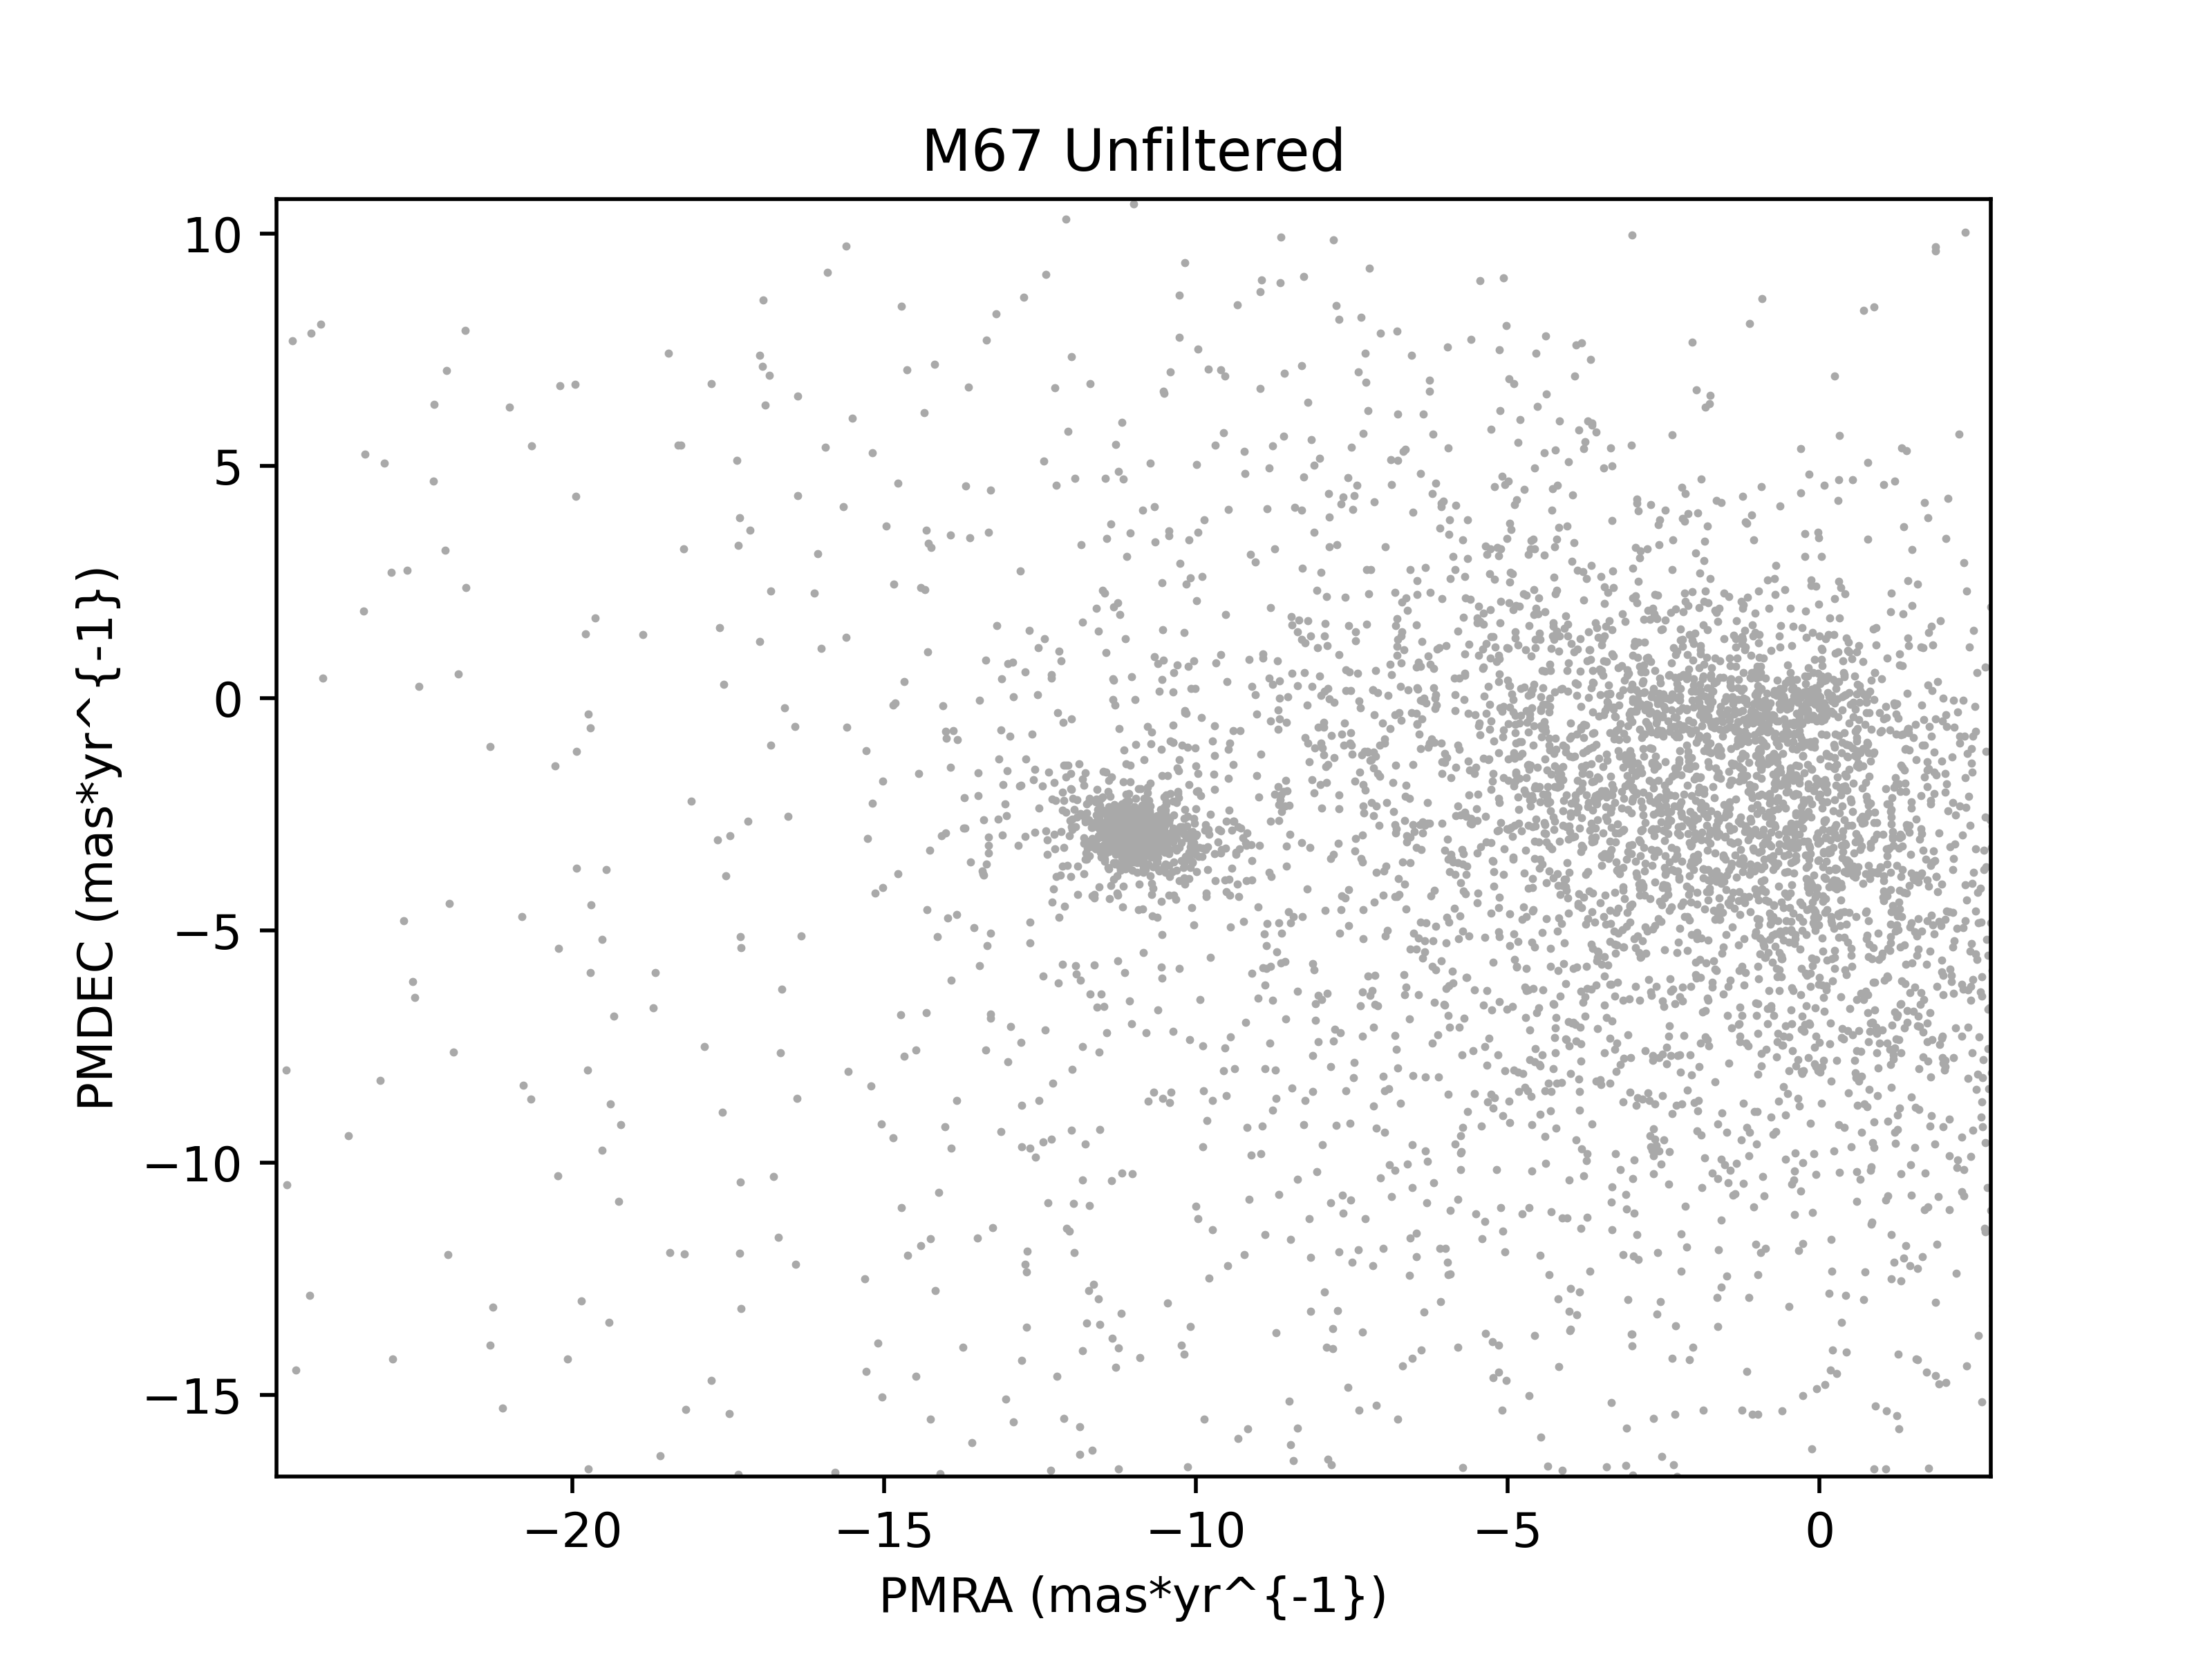
\includegraphics[width=4.75in]{figures/M67_pm_unfiltered.png}
	\caption{Diagram of the unfiltered proper motion space for the open cluster Messier 67. Horizontal axis tracks the proper motion in Right Ascension, and the vertical axis tracks the proper motion in Declination. The high density of points in the center is the identified proper motion spread for stars belonging to M67. The nebulous spread of points to its right are the random variations in proper motion in the Milky Way, roughly centered on (0,0).}
	\label{fig:M67_pm_unfiltered}
\end{figure}

With a proper motion concentration identified, we continue the filtering process by next looking only at stars brighter than magnitude 15. This is done to get a rough approximation for the cluster's mean properties, and we've found that the unfiltered brighter, upper main sequence tends to have lower fractional contamination. The entire data set reaches as faint as 20th magnitude, but the uncertainty in measurements tends to increase more dramatically in the fainter stars. I then apply a selection cut to the data, looking only at stars whose proper motion lies within the aforementioned clump. From this set of proper motion filtered bright stars, I calculate a mean and standard deviation for the parallax. Using these values, I then enforce a $1.5\sigma$ cutoff of parallax on the entirety of the data set, down to 20th magnitude. From this parallax filtered list of stars, I again filter by proper motion, resulting in a nearly final product. This method provides a list of stars who share a proper motion within the defined clump region, and a parallax withing 1.5 standard deviations of the mean for bright stars found within that clump.

The only additional filtering left is to remove especially 'noisy' measurements from the data set. Gaia provides a variable known as the \textit{astrometric\_sigma5d\_max}, which gives the length of the longest principal axis of the 5-dimensional error ellipsoid for the 5 given astrometric properties(RA, DEC, parallax, and proper motion in both RA and DEC). This $\sigma_{5D,Max}$ proves useful in estimating a bulk error in any of measurements used explicitly in the filtering process. As such, I cut off the post-filtration list of stars by a per-cluster defined cutoff, usually around  $\sigma_{5D,Max}=1$. This noise-based cut marks the end of the filtering process for a given cluster, and any star contained in the filtered list is assumed to be a member of the cluster for purposes of further analysis.

To empirically determine the quality and accuracy of filtering, we turn to another metric. As discussed in Section \ref{sec:hr}, a population of stars that formed at roughly the same time, from a cloud of gas and dust of roughly the same chemical abundances, should show a clear main sequence on a color-magnitude diagram (CMD). Constructing a CMD of unfiltered data, such as seen in Figure \ref{fig:M67_cmd_unfiltered}, we can see that a main sequence is present, but there are many 'contaminant' stars that do not belong to the same stellar population as our cluster of interest. We can use the 'cleanliness' of the main sequence and its turnoff point to gauge how well filtered a cluster is, though the balance between eliminating non-members and preserving as many stars from the true cluster as possible can be difficult. That being said, with the astrometry that guides the filtering process being somewhat independent of the photometry of a given star, over-constraining proper motion and parallax tends to thin out the main sequence rather than erase particular features. This is to say that putting too narrow or off-target a cut on proper motion would result in a more sparsely populated CMD, but features across the main sequence would still be present.

\begin{figure}[]
	\centering
      \includegraphics[width=4.5in]{figures/M67_cmd_unfiltered.png}
	\caption{HR diagram of the open cluster messier 67, constructed using unfiltered data and therefore including a high proportion of non-members. This particular construction of the HR diagram is often and henceforth referred to as a Color-Magnitude Diagram (CMD), owing to its principal axes being color index (BP-RP) and G-band magnitude. We choose to highlight M67 because its main sequence is easily visible even in an unfiltered CMD, but this is not the case in most other open clusters.}
	\label{fig:M67_cmd_unfiltered}
\end{figure}


To better demonstrate this filtering process, we use the example of a more crowded line of sight around Messier 35. Figure \ref{fig:M35_cmd_unfiltered} shows the CMD of an unfiltered view in a 1 degree radius around M35. A general trend of a main sequence is perhaps visible, but by no means conclusive enough to have any information drawn from it. Figure \ref{fig:M35_cmd_filtered_par} shows the effect of filtering the entire data set by the $1.5\sigma$ cutoff of parallax, as determined from the proper motion clump of only the bright stars. While parallax is considered to be the secondary tool to proper motion, this figure demonstrates how effective a good parallax measurement can be to further removing cluster non-members, especially on the brighter end of the data set. Finally, Figure \ref{fig:M35_cmd_filtered} shows the final product, with parallax, proper motion, and noise clipping in full effect. Depending on the quality of the fully filtered CMD and its intermediary stages, tweaks are often made to balance the removal of non-members and the preservation of cluster members and a main sequence. The corresponding breakdown of plots for other clusters worked on in this project can be found in the Appendix.

In the case of globular clusters, our ability to filter them to the same degree of confidence as that of open clusters is severely hindered by a few factors. Globular clusters are, by nature, much more dense than open clusters. As a result, it is difficult to resolve individual stars in some globular clusters, especially near the core. This makes it difficult to get accurate astrometric measurements to filter out foreground and adjacent non-members. Additionally, many globular clusters are sufficiently far away that the fractional uncertainty in the reported measurements is high, lowering out confidence in quality of filtration. Nevertheless, we've filtered several globular clusters in addition to the 15 open clusters analyzed in this work.  Figure \ref{fig:M15_cmd_unfiltered} shows the unfiltered CMD of Messier 15, and Figure \ref{fig:M15_cmd_filtered} shows the post-filtration CMD.

\begin{figure}[]
    \centering
      \includegraphics[width=4.75in]{figures/M35_cmd_unfiltered.png}
    \caption{Unfiltered CMD from the region surrounding Messier 35. No easily identifiable main sequence is visible, so it is clear that a robust method of identifying members of the cluster will be necessary. The color indices and magnitudes are displayed as reported by the Gaia archive, no further corrections or adjustments applied.}
    \label{fig:M35_cmd_unfiltered}
\end{figure}

\begin{figure}[]
    \centering
      \includegraphics[width=4.75in]{figures/M35_cmd_bright_filtered.png}
    \caption{Partially-filtered CMD of the region surrounding Messier 35. The data have been artificially cut off at 15th magnitude, and filtered by means of selecting stars in the high proper motion density region like the one identified in Figure \ref{fig:M67_pm_unfiltered}. This serves as an intermediate filtration step, and allows for the determination of estimate values for the cluster's parallax and apparent size.}
    \label{fig:M35_cmd_bright_filtered}
\end{figure}

\begin{figure}[]
    \centering
      \includegraphics[width=4.75in]{figures/M35_cmd_parallax_filtered.png}
    \caption{Parallax-only filtered CMD of the region surrounding Messier 35. The parallax cutoff range was selected from the mean and standard deviation of the parallaxes observed in the stars in Figure \ref{fig:M35_cmd_bright_filtered}. This step serves as an intermediate step in the cluster member filtration process. The success of the filtering of the upper main sequence is quite impressive, but there is still much contamination in the lower main sequence.}
    \label{fig:M35_cmd_filtered_par}
\end{figure}

\begin{figure}[]
    \centering
      \includegraphics[width=4.75in]{figures/M35_cmd_filtered.png}
    \caption{Final product of the cluster member filtration process, this CMD includes all of the stars believed to be members of Messier 35. The final set of members was identified through a sequential parallax and proper motion filtration process, with a final cut to the lower end of the main sequence if/where the compounded uncertainties rise sharply.}
    \label{fig:M35_cmd_filtered}
\end{figure}

\begin{figure}[]
    \centering
      \includegraphics[width=4.75in]{figures/M15_cmd_unfiltered.png}
    \caption{Unfiltered CMD from the region surrounding globular cluster Messier 15. M15 was one of the most easily processed globular clusters, as the field of view around it features relatively few contaminating non-members in comparison to some of the other globular clusters we surveyed.}
    \label{fig:M15_cmd_unfiltered}
\end{figure}

\begin{figure}[]
    \centering
      \includegraphics[width=4.75in]{figures/M15_cmd_filtered.png}
    \caption{Fully filtered CMD of the globular cluster Messier 15. The population of stars belonging to a globular cluster are quite old relative to many younger, open cluster populations. As such, the features of the CMD are much different in that of a globular cluster. There is little remaining of the main sequence, with a clear red, asymptotic, and even horizontal giant branch visible. Many open cluster isochrones include these features for use in fitting, but very few observed open cluster CMDs bear them.}
    \label{fig:M15_cmd_filtered}
\end{figure}

\section{Heart of the Data} \label{sec:dataUse}

With all of the filtering processes completed, and a confident list of cluster members identified, we analyze and tackle the  heart of the data. Looking at the features of the HR diagram on a filtered CMD, labeled for example using Messier 67 in Figure \ref{fig:M67_cmd_filtered_labeled}, we can observe a few phenomena. First, we have the main sequence. Seeing observational main sequences that roughly line up with those in theory is reassuring. That being said, even mixed, unfiltered populations of stars will tend to trace out a main sequence. What makes the filtered CMD main sequence promising is the thin, well defined main sequence and its turnoff. The turnoff from the main sequence, as discussed in Section \ref{sec:hr}, is a reflection of the general age of the cluster. The position of the main sequence in general, and the shape that it takes, has to do a lot with the elemental abundances in the stars when they were formed, which we call metallicity. Above the main sequence, where the cluster's CMD appears to fold in on itself, we observe the ascent of stars into the red giant branch. Most open clusters are relatively young, around 1 Gyr or less in age, and as such do not present many features past the main sequence turnoff. In older open clusters, and in most globular clusters, we can see the continuation of stars past the red giant branch and into the asymptotic giant branch and horizontal branch phases. The presence of these features on a CMD can provide much more information, but also presents an increase challenge to fit models to and accurately characterize.

\begin{figure}[]
    \centering
      \includegraphics[width=4.75in]{figures/M67_cmd_filtered_labeled.png}
    \caption{Labeled CMD of the open cluster Messier 67. All points shown are stars that are believed to be members of the cluster, and were identified in the same manner as detailed for M35 in Section \ref{sec:filtering}.}
    \label{fig:M67_cmd_filtered_labeled}
\end{figure}

Additional features that can be seen in some CMDs, again as labeled in Figure \ref{fig:M67_cmd_filtered_labeled}, are the red clump and blue stragglers. In contrast to the relatively sparse spread of stars that lie past the main sequence turnoff point, a higher density of stars can be seen clumped together. This red clump is created by lower mass stars that are evolving off the main sequence, with their hydrogen core having fused into a core of helium. The stars build up a core of helium until a point where the conditions are right for helium fusion to spontaneously begin, known as a helium flash. Stars tend to spend a longer time in the helium fusing stage compared to other stages past the main sequence, causing a higher density of points on the CMD relative to the other stages past the main sequence turnoff. As for the case of blue stragglers, a less dense string of stars can be observed to continue past the main sequence turnoff, almost appearing to extend the main sequence past its typical conclusion. This region of the CMD is host to stars known as blue stragglers. The exact origin of these blue stragglers is not known, but the most plausible explanation is that these stars formed later than the majority of the stars in the cluster, giving them a similar metallicity but a younger age. For a cluster as old as Messier 67, we would expect stars on this region of the CMD to have already burned past their main sequence lifespan, thus giving rise to the turnoff and post turnoff regions of the CMD.

A final feature of note is the apparent spread of points that lies above the lower main sequence, which in some clusters gives the appearance of there being two main sequences. The higher magnitude, or fainter edge of the lower main sequence has a more dense, well defined edge to it. Conversely, the brighter edge to this main sequence spread is less well defined and less dense. The reason for this spread in the main sequence is likely due to the presence of binary stars. These binaries are a system of two stars that are orbiting close to each other, and are therefore often observed as a single star. If these two stars were to have roughly the same color index and magnitude, then when observed side by side the 'single' star will appear to be twice as bright as a star of its color index should be. Because of how the logarithmic magnitude system is defined, a doubling of the brightness of a star would correspond to a change of 0.75 magnitudes. Any differences in relative mass or partial occultation of one star by the other would result in a star appearing somewhere between the main sequence and the point 0.75 magnitudes brighter. To demonstrate this, Figure \ref{fig:MS_spread} shows a linear fit to a main sequence, and its twice as bright counterpart. A majority of the stars in the main sequence spread appear to fall within this window between the main sequence and the binary sequence, giving credibility to this explanation.

\begin{figure}[]
    \centering
      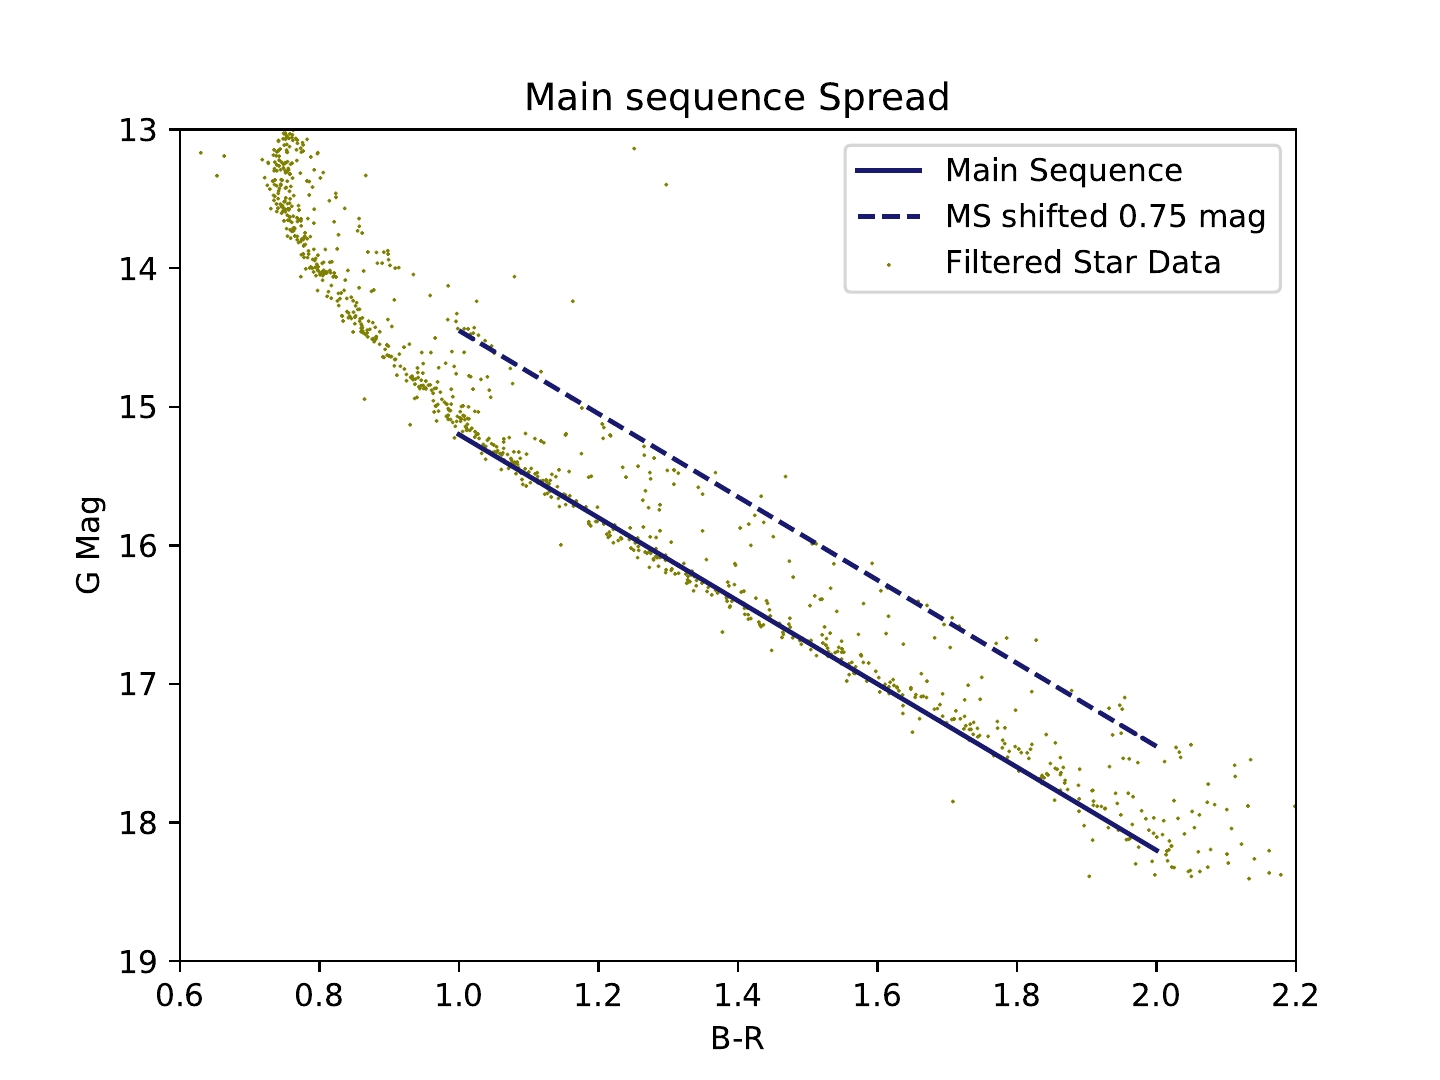
\includegraphics[width=4.75in]{figures/M67_MS_spread.png}
    \caption{Augmented CMD of Messier 67, with an approximate linear fit to the main sequence shown in solid red. Directly above it by 0.75 magnitudes, which is equivalent to double the source intensity, is the binary sequence. This binary sequence marks what is in theory the upper edge for main sequence stars with an unresolved binary companion.}
    \label{fig:MS_spread}
\end{figure}

\subsection{Isochrones} \label{sec:iso}
In order to better characterize these open clusters, using their color magnitude diagrams, we look to stellar evolution models. CMDs constructed from these models are called isochrones, and can be used to infer properties of stars and stellar clusters that were not directly measured. In this case, finding an isochrone that roughly follows the main sequence and turnoff of one of our clusters would allow us to infer an approximate age and metallicity of that cluster. Before this best fitting analysis can be done, however, there are a few factors to consider.

Measurements given in the magnitude system are not necessarily equal. In addition to the passband or range of wavelengths the magnitude is specified over, we have to consider apparent versus absolute magnitude. Due to the inverse square law, detailed in Equation \ref{eq:invsqlaw}, light drops off as a function of the distance squared. Because of this, the apparent magnitude of a star, or how bright it is measured to be, will decrease the further away the star is. Thankfully, Gaia includes measurements of trigonometric parallax, from which we can derive a distance estimate. Given the distance, it is easy enough to standardize the brightness of all stars to how bright they would be at a fixed distance, chosen to be 10 parsecs by convention, which we call the absolute magnitude. Isochrone `measurements' are given in absolute magnitudes, so before any meaningful comparison can take place it is necessary to convert the Gaia measurements to absolute magnitude. This is done using the distance modulus, shown in Equation \ref{eq:dist_mod}, where m and M represent the apparent and absolute magnitudes, respectively. The distance d is calculated in parsecs from the parallax measurements reported by Gaia.

\beq
\label{eq:invsqlaw}
I = \frac{I_0}{4\pi r^2}
\eeq

\beq
\label{eq:dist_mod}
m - M  = 5\cdot log_{10}\left(d\right) - 5
\eeq

Another issue that affects the attempt to compare isochrones to observed CMDs is interstellar extinction. Gas and dust that lie between the observer and the source can scatter and absorb some of the light, causing objects to be observed as fainter than they should at their given distance. Additionally, the dust grains in the interstellar medium tend to scatter shorter wavelengths more efficiently. The result of this is that shorter wavelengths, or more blue light, are extinguished and scattered more readily than longer, more red wavelengths. This phenomena is accordingly named interstellar reddening, and is an additional feature to consider on top of extinction. There is generally a proportional relationship between the amount of extinction and the amount of reddening. In the case of the passbands used in this work, the constant of proportionality is roughly 2.1 times the extinction in magnitudes for every unit of color excess. We determined this empirically from the member populations of Messier 67 and Messier 35, for which Gaia estimates the color excess factor.

\beq
\label{eq:extinction}
A_G = R_G \cdot E\left(BP-RP\right), \quad R_G \approx 2.1
\eeq

The isochrones chosen for use in this work come from the MESA Isochrones \& Stellar Tracks (MIST) project\protect{\cite{mist}}. The MIST models provide synthetic photometry in the Gaia passbands, as well as effective temperature, mass, metallicity, and more for each model star. The MIST models trace out the important main sequence and turnoff, but also features like the red giant branch, horizontal branch, and asymptotic branch. This means that the set of isochrones are versatile in fitting to a broad variety in both open and globular clusters. In Figure \ref{fig:iso_trends}, we can see the effects of changing age and metallicity, respectively. Accounting for reddening and extinction will also serve to slide each isochrone along a diagonal line, with a slope of $-2.1$.

\begin{figure}[]
    \centering
      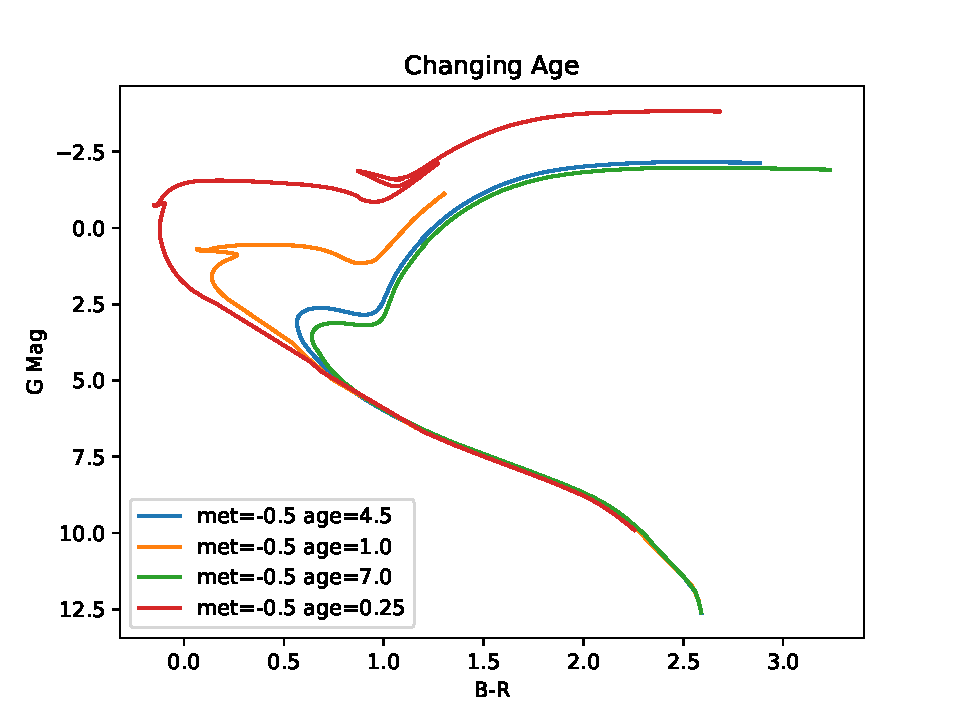
\includegraphics[width=3.5in]{figures/iso_age.pdf}
      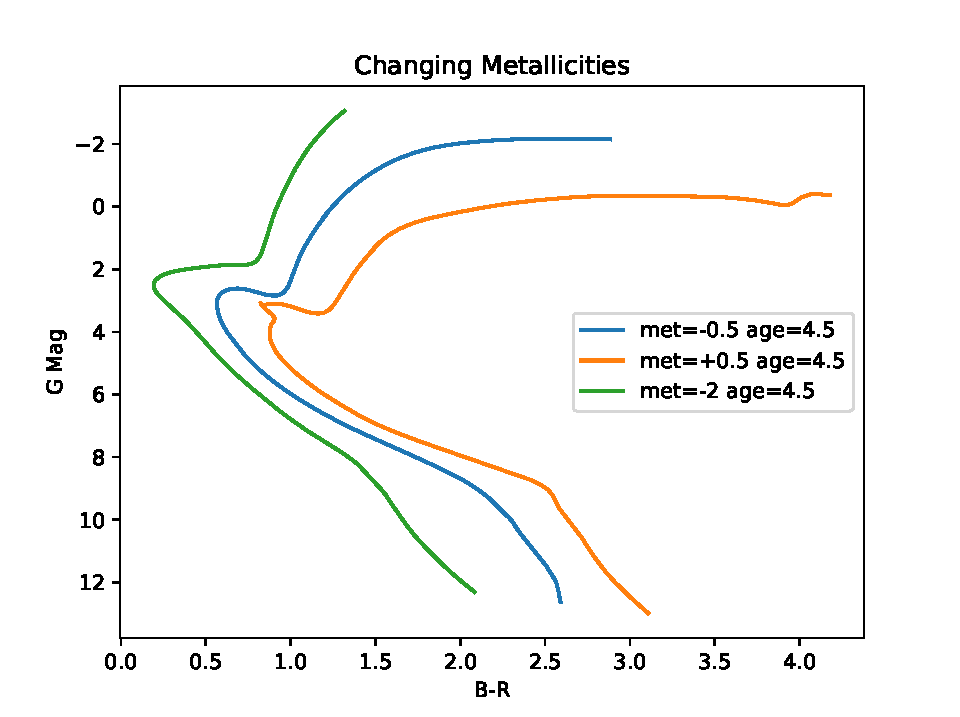
\includegraphics[width=3.5in]{figures/iso_metallicity.pdf}
    \caption{Demonstration of the trends in changing the two primary variables in the isochrone model set. \textbf{Left:} Changing the age at a constant metallicity shifts the location of the main sequence turnoff point to the lower right corner, which represents a fainter and more red population of stars. \textbf{Right:} Changing metallicity at a constant age shifts the color index of the entire HR diagram, and changes many features like the shape of the main sequence and its post-turnoff region. The combination of changes in these two variables is what is used to fit models to the observed cluster data.}
    \label{fig:iso_trends}
\end{figure}

\subsection{Fitting} \label{sec:fit}
With all of the corrections and possible variables to account for in mind, the process of automating the search for a best-fitting isochrone is not easy. A brute force comparison of all possible combinations of the isochrones to every observed cluster member is not feasible, and so our solution is to reduce the number of points being analyzed. In an effort to create a small but spatially representative number of points as a proxy for fitting, we use a routine to divide the CMD into equally sized horizontal slices. The mean color index and magnitude of all of the stars in this bin are taken to be a representative proxy star. The list of proxy stars, usually of order 50 points, therefore traces out the main sequence and turnoff while significantly reducing the number of comparison points. One benefit of this method of analysis is that the turnoff, which is arguably one of the most important features in determining goodness of fit, is represented with the same density of points as the main sequence. In most cases of the observed CMD, the main sequence has several orders of magnitude more stars than the turnoff region, and so would be over-fitted in a brute force approach. In the case of some clusters, this automated proxy point assignment routine does not create an effective outline of the main sequence and turnoff by eye, or leaves out key features. In these cases, a manual override of placing proxy points on an interactive plot is used instead, to ensure a more successful fitting routine downstream. An example of the proxy point assignment can be found in Figure \ref{fig:M67_cmd_proxy}.

\begin{figure}[]
    \centering
      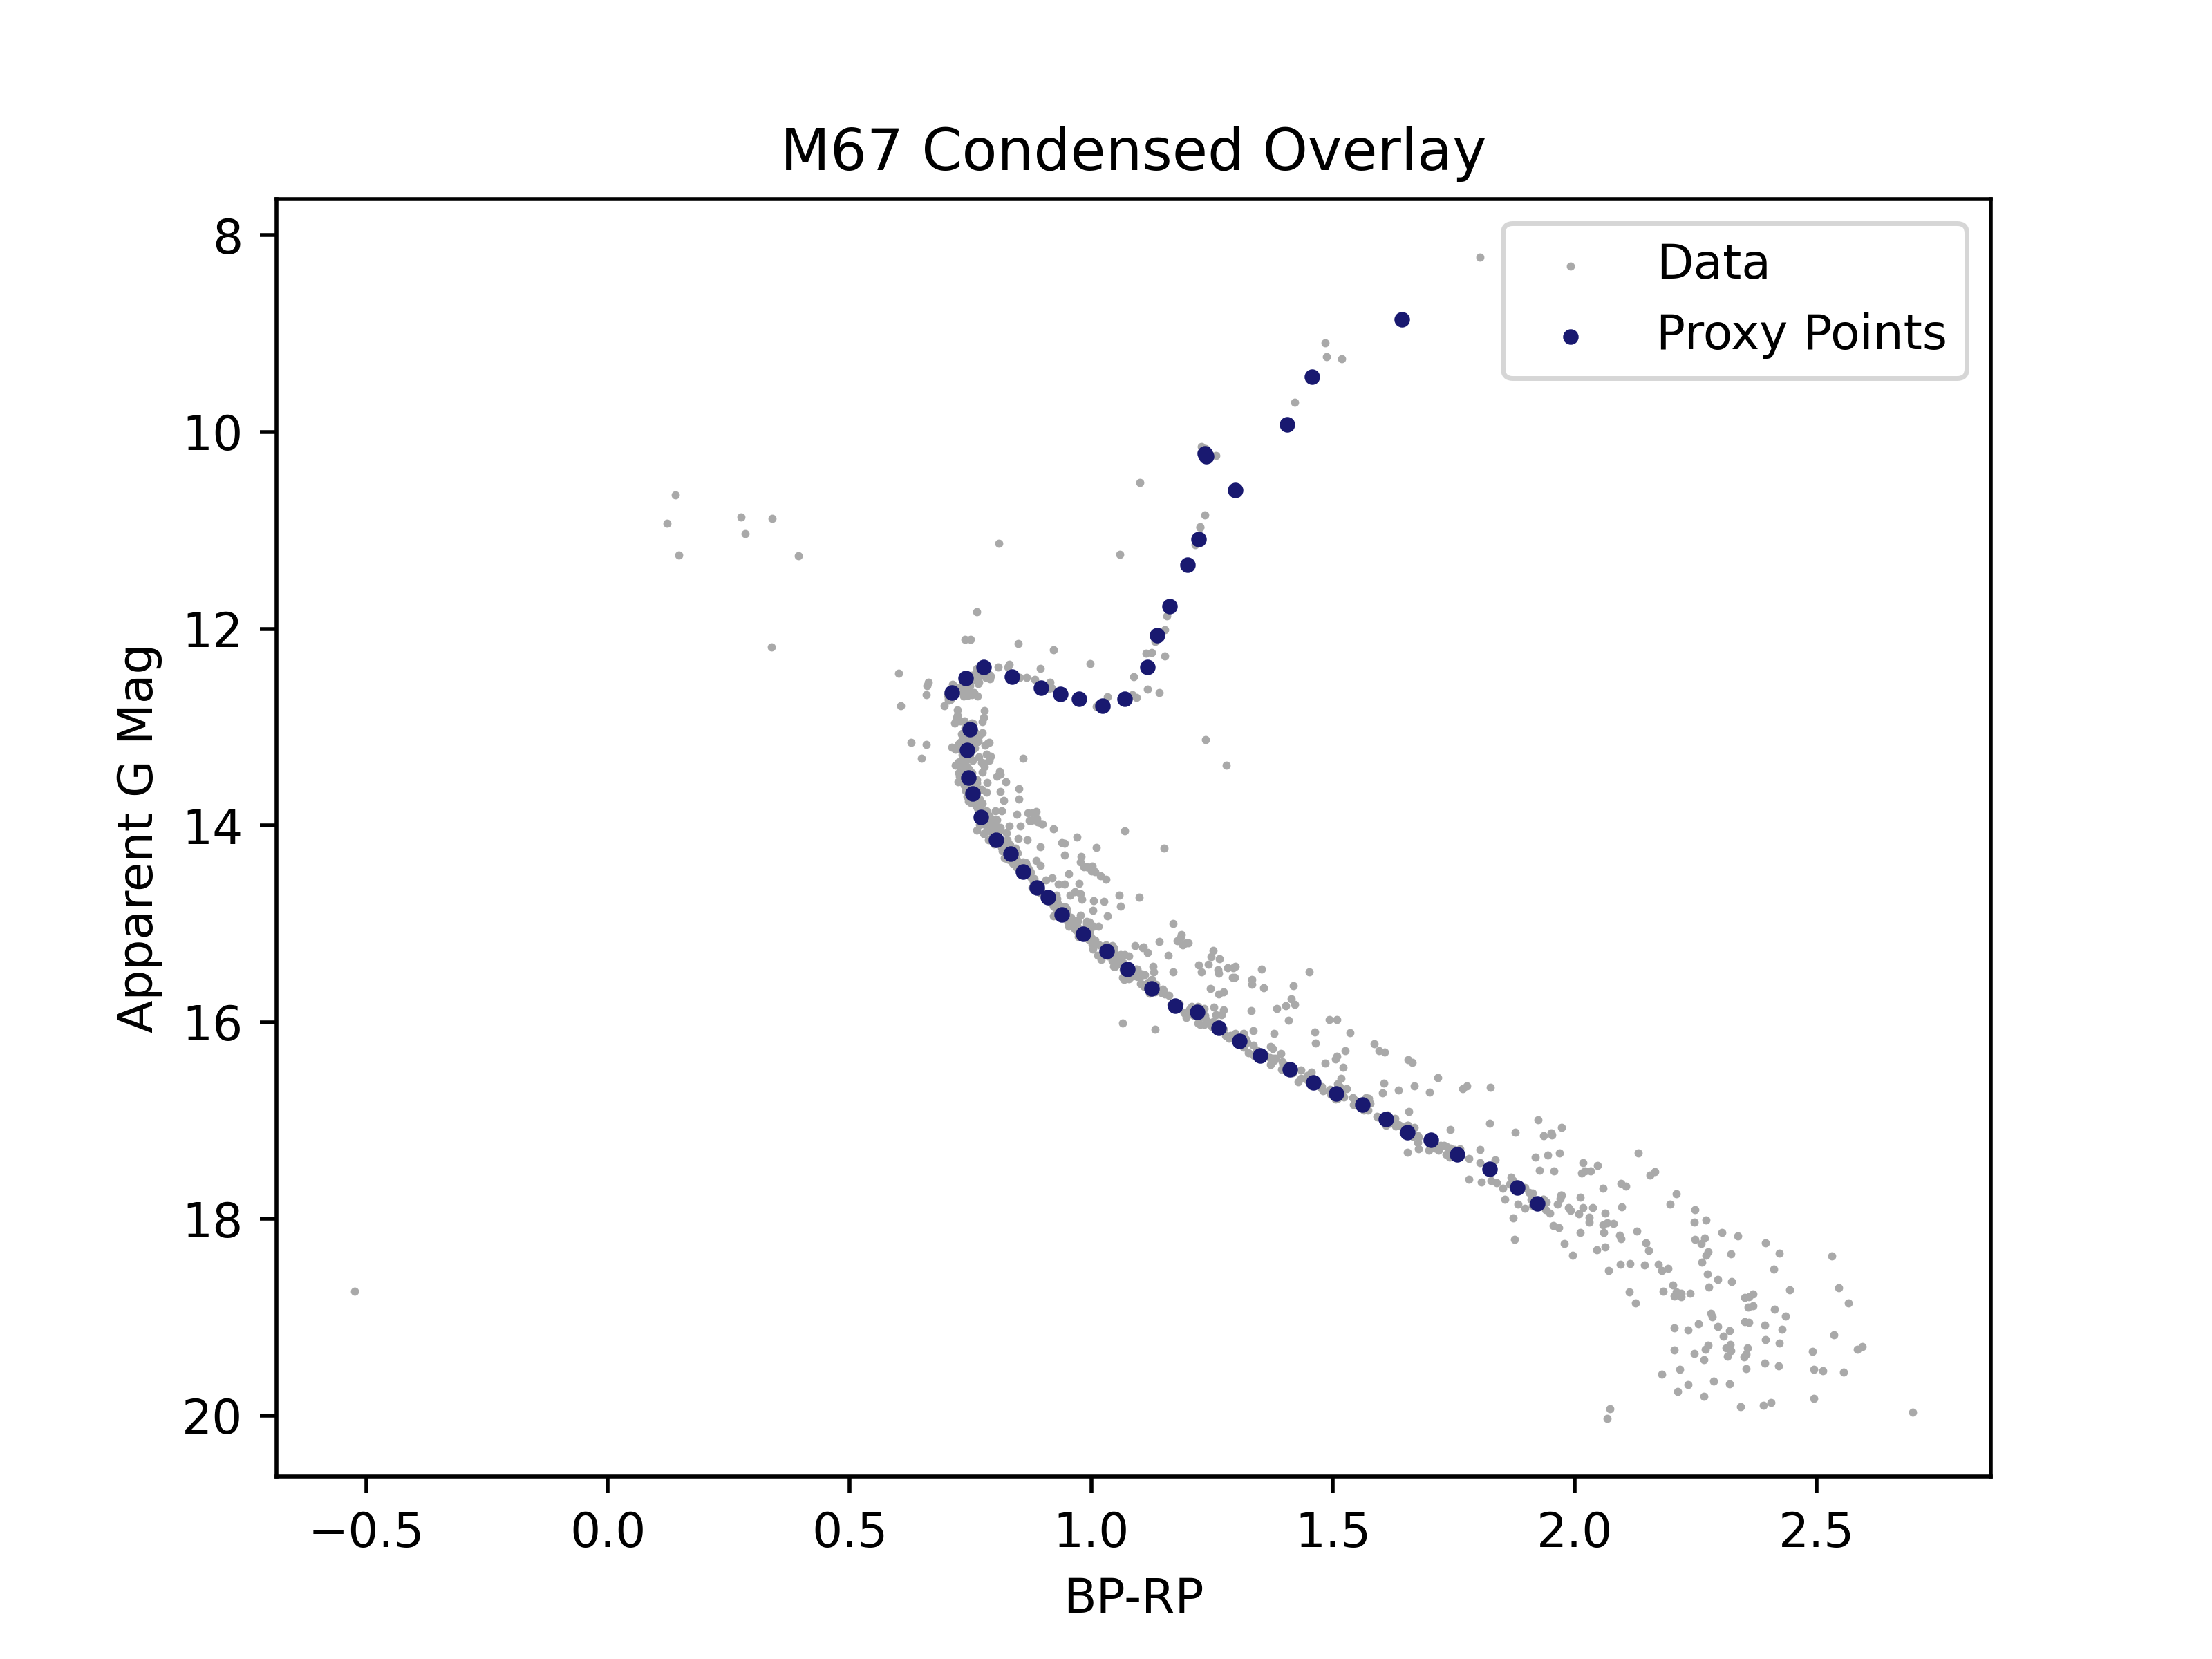
\includegraphics[width=4.75in]{figures/M67_condensed_CMD_overlay.png}
    \caption{CMD of the identified cluster members in Messier 67. The proxy points used for the isochrone fitting process are shown in dark blue, and in this case were placed manually to ensure accurate recreation of the post-turnoff features.}
    \label{fig:M67_cmd_proxy}
\end{figure}

With a list of proxy points for use in fitting, the next step is to find a metric for the goodness of fit. After some trial and error, we determined that the sum of the squared distances between proxy points and the isochrone was our best metric. Minimizing this metric, shown in Equation \ref{eq:gof}, provides a best fit isochrone that statistically weights each proxy point equally. In this equation, $x_m$ and $y_n$ represent each proxy point. $x_{iso}$ and $y_{iso}$ represent the nearest point on the isochrone to each proxy point. Experiments with weighting proxy points higher in the brighter end of the main sequence and post-turnoff regime demonstrated minor improvements to best fit models for some clusters, but worse fits for other clusters. As such, a weighting scheme is not used on an individual proxy point basis, and rather a manual assignment of proxy points is used to emphasize key features of the CMD if the automated proxy point assignment does not produce a good fit by eye.

\beq
\label{eq:gof}
G.O.F = \sum\limits_{n=1}^{N}\left[\left(x_n-x_{iso}\right)^2+\left(y_n-y_{iso}\right)^2\right]
\eeq

With a goodness of fit metric selected, the main challenge becomes covering the efficient coverage of the parameter spaces. The current MIST release includes 1155 unique isochrones. These isochrones vary in age and metallicity, the latter of which is expressed in the logarithmic ratios of several chemical abundances, normalized to solar abundance. $[\frac{Fe}{H}]$ gives the logarithm base 10 of the ratio of all Iron species relative to Hydrogen, with $[\frac{Fe}{H}]=0$ being solar abundance. For the MIST isochrones, $[\frac{Fe}{H}]$ is represented in steps of 0.5 from -4 to -2, and steps of 0.25 from -2 to +0.5. An additional measurement of metallicity is given in $[\frac{\alpha}{Fe}]$, again normalized to a solar abundance of 0. $[\frac{\alpha}{Fe}]$ compares the abundance of one or several alpha process elements to Iron. Previous isochrone models that were sampled varied $[\frac{\alpha}{Fe}]$ by $\pm 0.5$, but the current iteration of MIST models uses exclusively $[\frac{\alpha}{Fe}]=0$. The final variable tracking chemical abundances is $y$, which gives the mass fraction of Helium in the star. MIST isochrones vary in $y$ from around 0.25 to around 0.31. They also vary in the simulated age, ranging from 1 Myr up to 20 Gyr, with the steps in age between each isochrone increasing with cumulative age.

Fitting three variables creates an increasingly large number of permutations. To reduce the computation time, we first search over the range of reddening from 0 to 0.5 in steps of 0.05, evaluating the goodness of fit for all 1155 isochrones at each step. Once the best fit is identified, a final pass of reddening $\pm 0.05$ from the best fit, done in increments of 0.01, is used to fine-tune the estimation of reddening and extinction. The isochrone list is then again sorted by goodness of fit and the best fit identified. The full list of sorted permutations, 26565 elements in length, is saved efficiently for later recall. We also use an interactive plot to step through all three parameter spaces to visualize the best fit and its nearest neighbors in the parameter spaces. This method of fitting is surprisingly quick and effective, especially so in the case of open clusters. Despite this challenge of fitting many different types of clusters, our automated fitting routine has been robust at identifying what we agree to be the best fit by eye. The best-fit parameters for 16 open clusters are tabulated in Table \ref{tab:fits}.


\begin{table}[]
\centering
\rowcolors{2}{white}{gray!25}
\begin{tabular}{llllll}
\toprule
Cluster ID & Distance (pc) & Members & Age (Gyr) & $[\frac{Fe}{H}]$ & E(BP-RP) \\ \midrule
IC4651     & 943        & 950     & 1.585     & 0.50             & 0.04      \\
M35        & 871        & 1231    & 0.056     & 0.00             & 0.46      \\
M46        & 1668       & 2000    & 0.398     & 0.25             & 0.17      \\
M47        & 479        & 470     & 0.045     & 0.00             & 0.25      \\
M48        & 759        & 638     & 0.447     & 0.25             & 0.02      \\
M50        & 973        & 908     & 0.063     & 0.00             & 0.44      \\
M67        & 873        & 1000    & 3.548     & 0.25             & 0.00      \\
NGC188     & 1940       & 802     & 5.012     & 0.50             & 0.00      \\
NGC2158    & 4659       & 767     & 1.259     & 0.00             & 0.54      \\
NGC2204    & 4896       & 138     & 1.413     & 0.25             & 0.00      \\
NGC2301    & 889        & 935     & 0.126     & 0.25             & 0.09      \\
NGC2355    & 1942       & 321     & 0.794     & 0.00             & 0.22      \\
NGC2360    & 1121       & 736     & 0.708     & 0.50             & 0.00      \\
NGC6633    & 381        & 264     & 0.708     & 0.25             & 0.11      \\
NGC6791    & 4140       & 1104    & 8.913     & 0.25             & 0.19      \\
NGC752     & 443        & 182     & 1.259     & 0.25             & 0.01      \\ \bottomrule
\end{tabular}
\caption{Summary of the results from our filtering and isochrone-fitting procedures. Uncertainties in many of the parameters are difficult to estimate, for reasons outlined in Section \ref{sec:uncertainty}.}
\label{tab:fits}
\end{table}


Many attempts were made to bridge this process, which is relatively well suited for the main-sequence dominated open cluster CMDs, to that of globular clusters. In the case of our best-filtered globular cluster, Messier 15, we can confidently assign a best fitting isochrone, shown in Figure \ref{fig:M15_iso}. Even in this case, however, our confidence in the inferred age of the cluster is low. The best-fitting isochrone bears a model age of over 15.8 Gyr, far older than the determined age of the universe. Moreover, other globular clusters had a best-fit determined age in the vicinity of 20 Gyr. As such, though we have great interest the comparison between open and globular clusters, we reluctantly ended the inclusion of globular clusters in the sample set at this stage. Though we are unable to publish conclusive findings on globular cluster population statistics, this topic is one which we have interest in studying more in future.

\begin{figure}[]
    \centering
      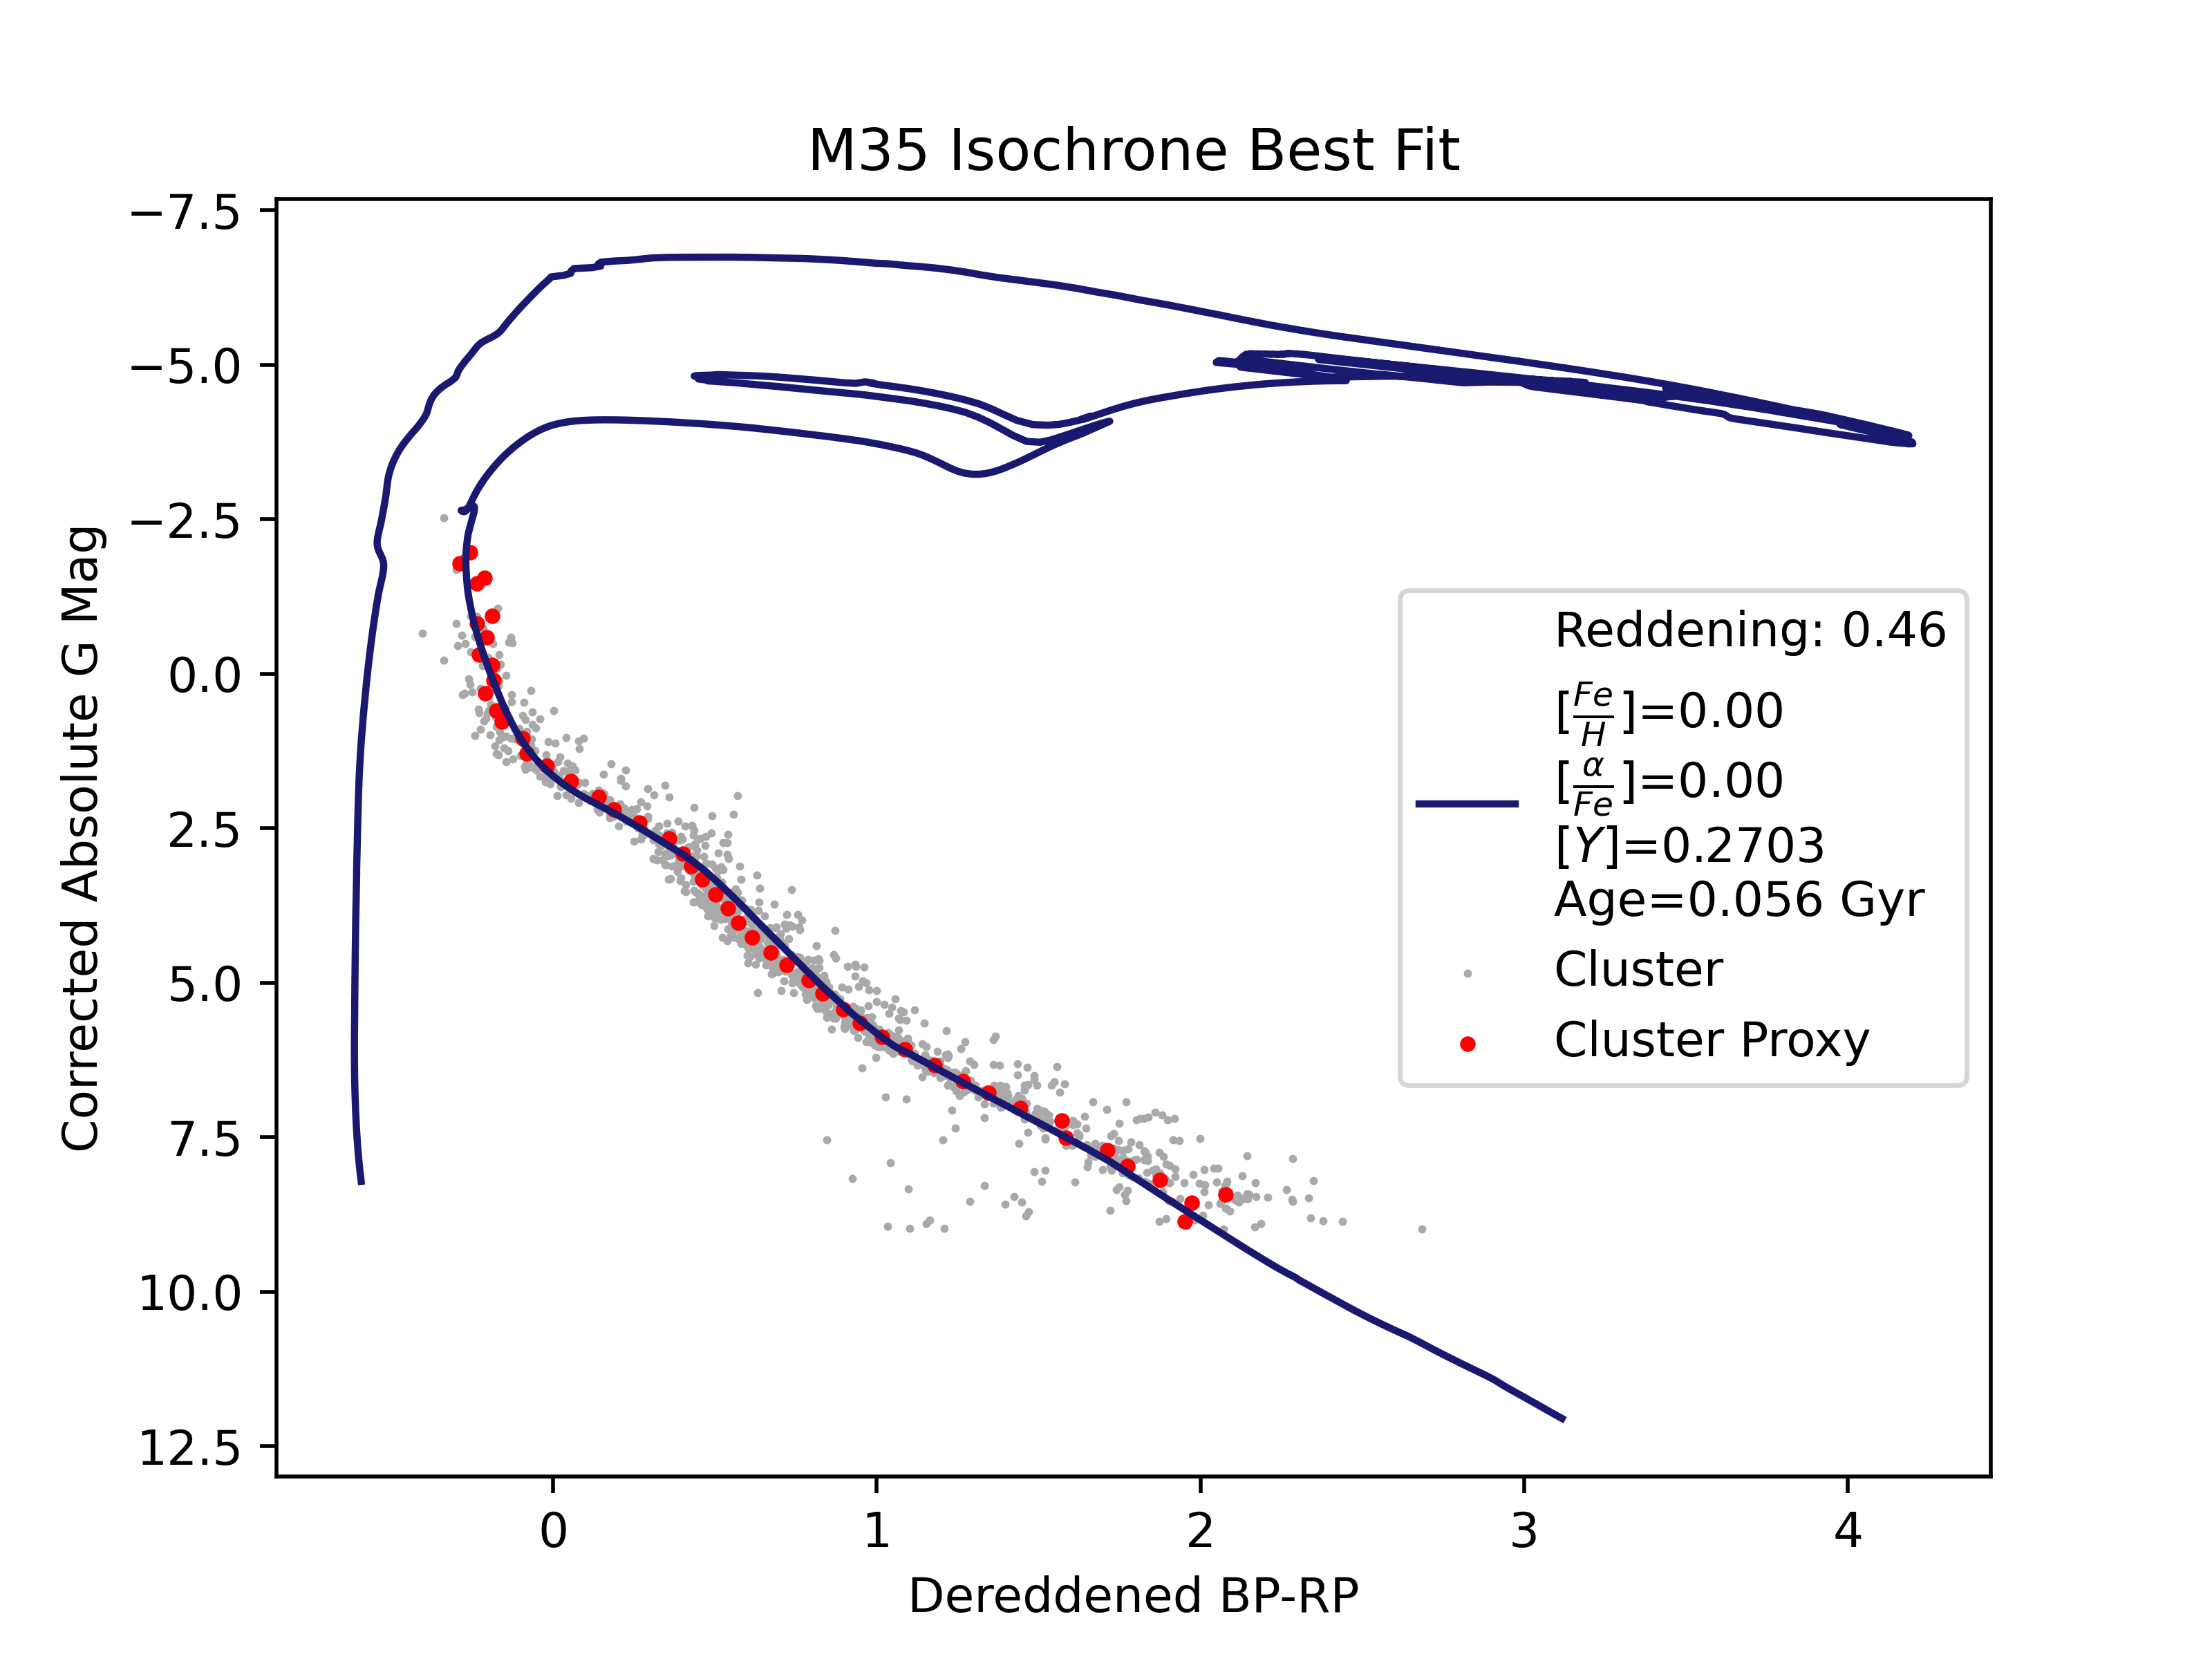
\includegraphics[width=4.75in]{figures/M35_CMD_Iso_BestFit.png}
    \caption{Filtered, distance corrected, and interstellar reddening/extinction corrected CMD of Messier 35 shown in gray. The red points are proxy points used in the fitting process for efficiency. The best fitting isochrone is overlaid in dark blue.}
    \label{fig:M35_iso}
\end{figure}

\begin{figure}[]
    \centering
      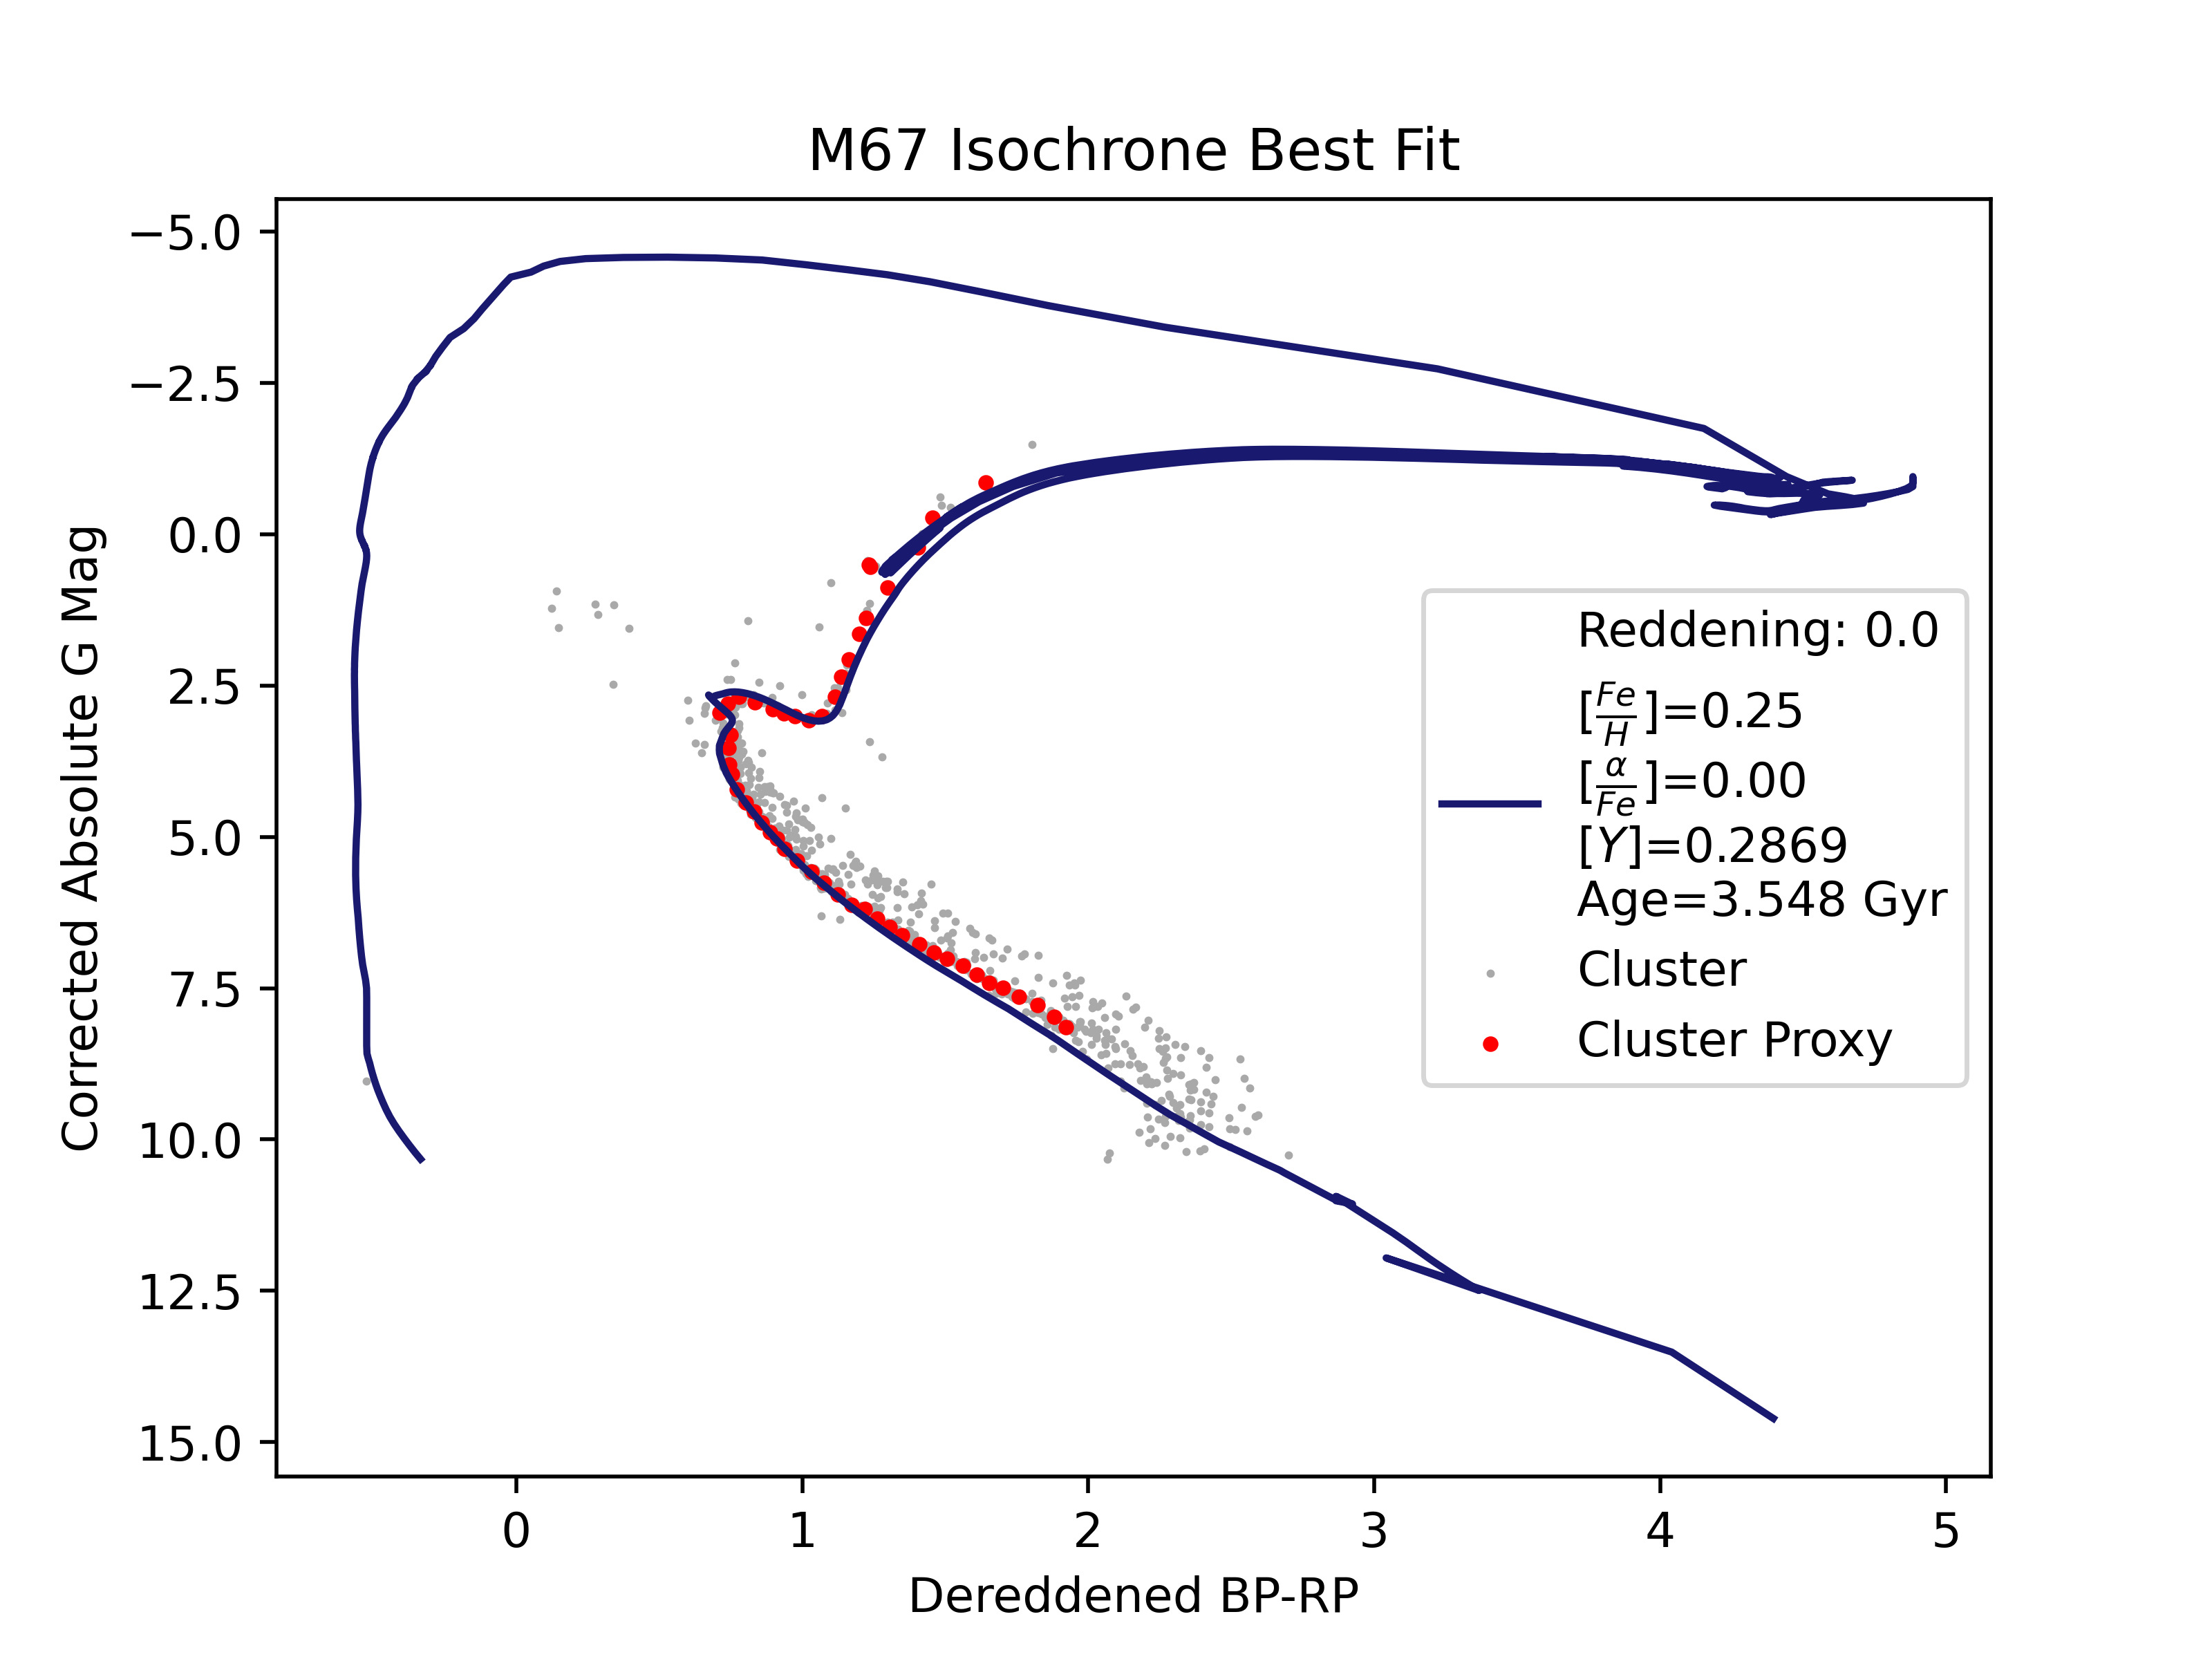
\includegraphics[width=4.75in]{figures/M67_CMD_Iso_BestFit.png}
    \caption{Filtered, distance corrected, and interstellar reddening/extinction corrected CMD of Messier 67 shown in gray. The red points are proxy points used in the fitting process for efficiency. The best fitting isochrone is overlaid in dark blue.}
    \label{fig:M67_iso}
\end{figure}

\begin{figure}[]
    \centering
      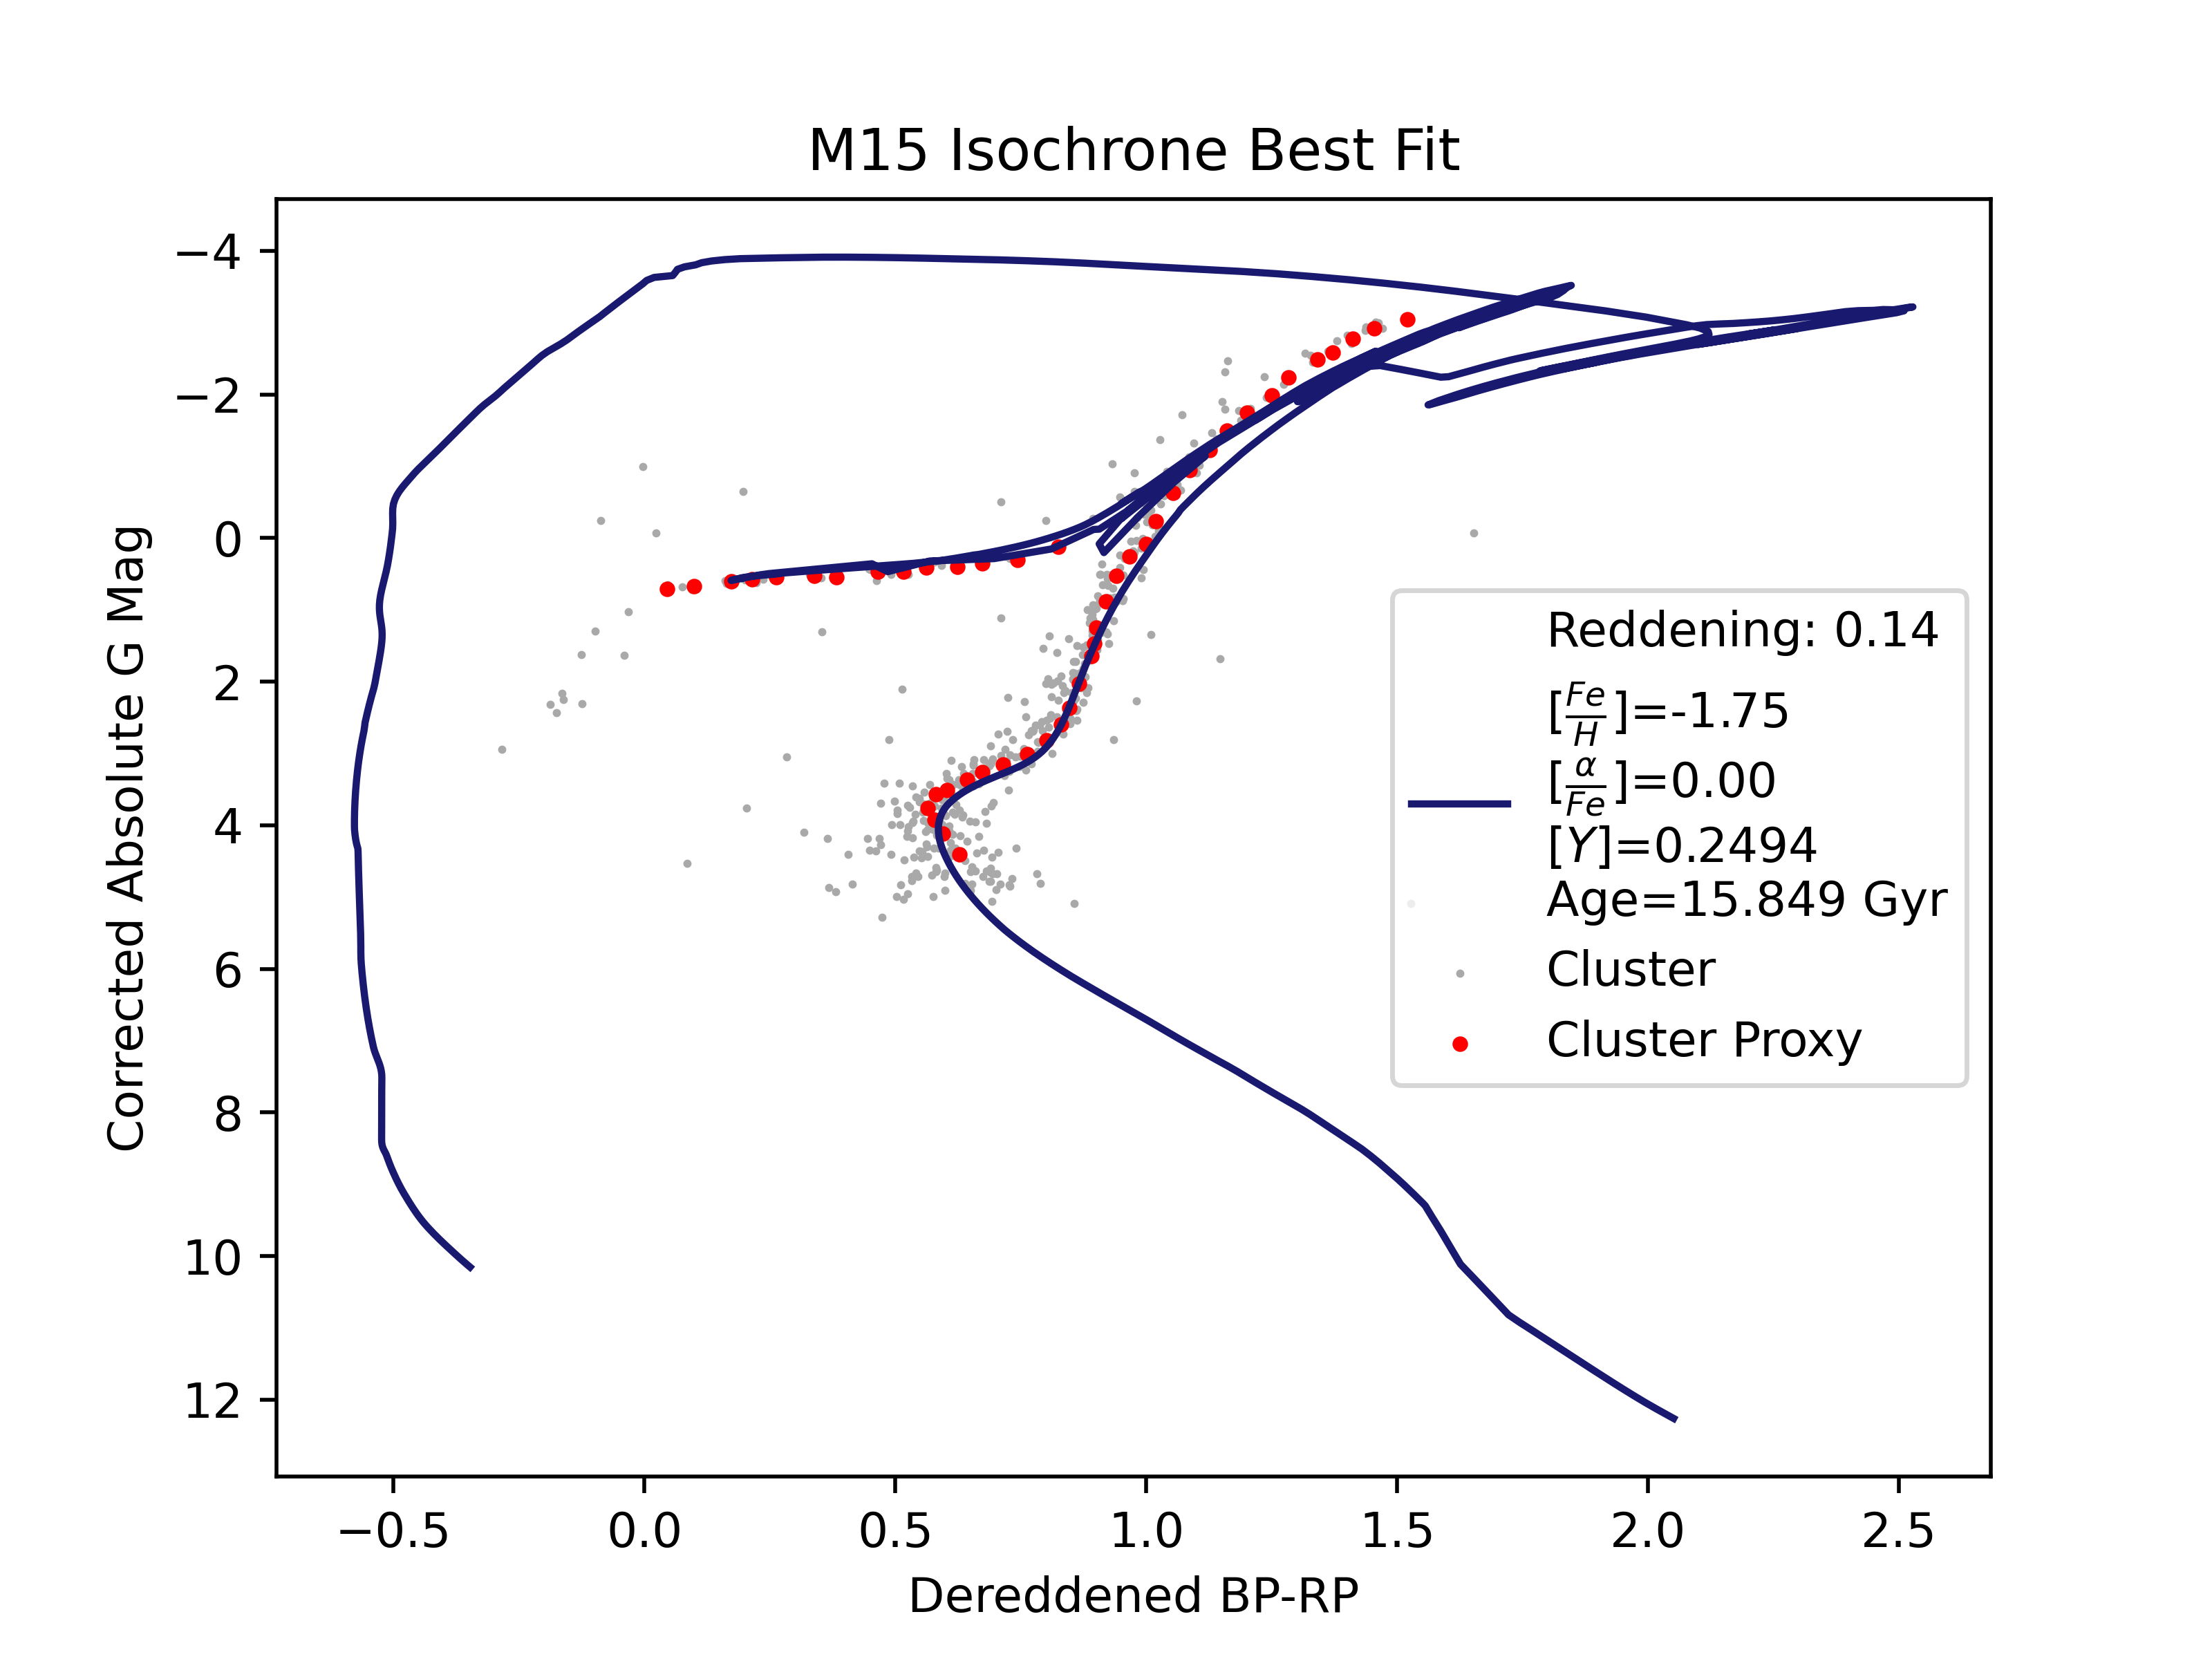
\includegraphics[width=4.75in]{figures/M15_CMD_Iso_BestFit.png}
    \caption{Filtered, distance corrected, and interstellar reddening/extinction corrected CMD of Messier 67 shown in gray. The red points are proxy points used in the fitting process for efficiency. The best fitting isochrone is overlaid in dark blue.}
    \label{fig:M15_iso}
\end{figure}

\section{Membership Profiles} \label{sec:membership}

With a filtered and isochrone-fit data set for each cluster, one of the key areas of interest that we explored was the density profiles of clusters. The main measurements needed to look at density profiles are the right ascension, declination, and parallax. Though the parallax measurements from Gaia come with impressively small uncertainties, the proportional error still makes accurate 3D mapping of dense clusters at high distances difficult. For example, we determined the cluster M67 to have a half-light radius of around 3 parsecs. However, the average cluster member of M67 has an uncertainty in parallax distance of order 20 parsecs. As such, in order to get the most precise radial membership profiles, we have gone with a 2D projected sky map model. The parallax measurements for stars identified as cluster members are flattened to the mean for the cluster, and their distance from the cluster center is calculated purely from measurements of right ascension and declination. We recognize that this has the disadvantage of potential inaccuracies in the mapping of non-uniformly dispersed clusters, but the uncertainty in parallax for distant clusters was too high to accurately project a 3D membership profile.

With a projected sky map in mind, the data was then sorted into radial bins, typically $N=100$, which form concentric rings around the cluster center. These rings are spaced equally in the RA, spanning the region from the center of the cluster to the furthest identified member. The center of the cluster is identified as the mean RA and DEC position of the filtering-identified cluster members. A small region in the center of these concentric radial bins, roughly the inner 5\% by radius, is excluded from any calculations in order to prevent overestimation of density given an exceedingly small effective area. Another deliberate adjustment is the over weighting of the central regions of the cluster. Of the total $N$ bins spanning the search area of radius $R$, $\frac{N}{2}$ or half of the radial bins lie within the inner $\frac{R}{4}$. This bias in the distribution of bin density was chosen to provide finer resolution in the center of the search region, since the search region tends to include a far wider area than what would be identified as the cluster by eye. While this only $\frac{R}{4}$ selection only represents $6.25\%$ of the total search region by area, we have observed that in the case of most open clusters, the density drops off to a near constant within a small portion of $R$. This observation also further motivated the functions we use to represent cluster density. A visualization of the separation of the bins, both in the central and external regions of the cluster, can be seen in Figures \ref{fig:radBins} \& \ref{fig:radBinsCenter}.

\begin{figure}[]
    \centering
      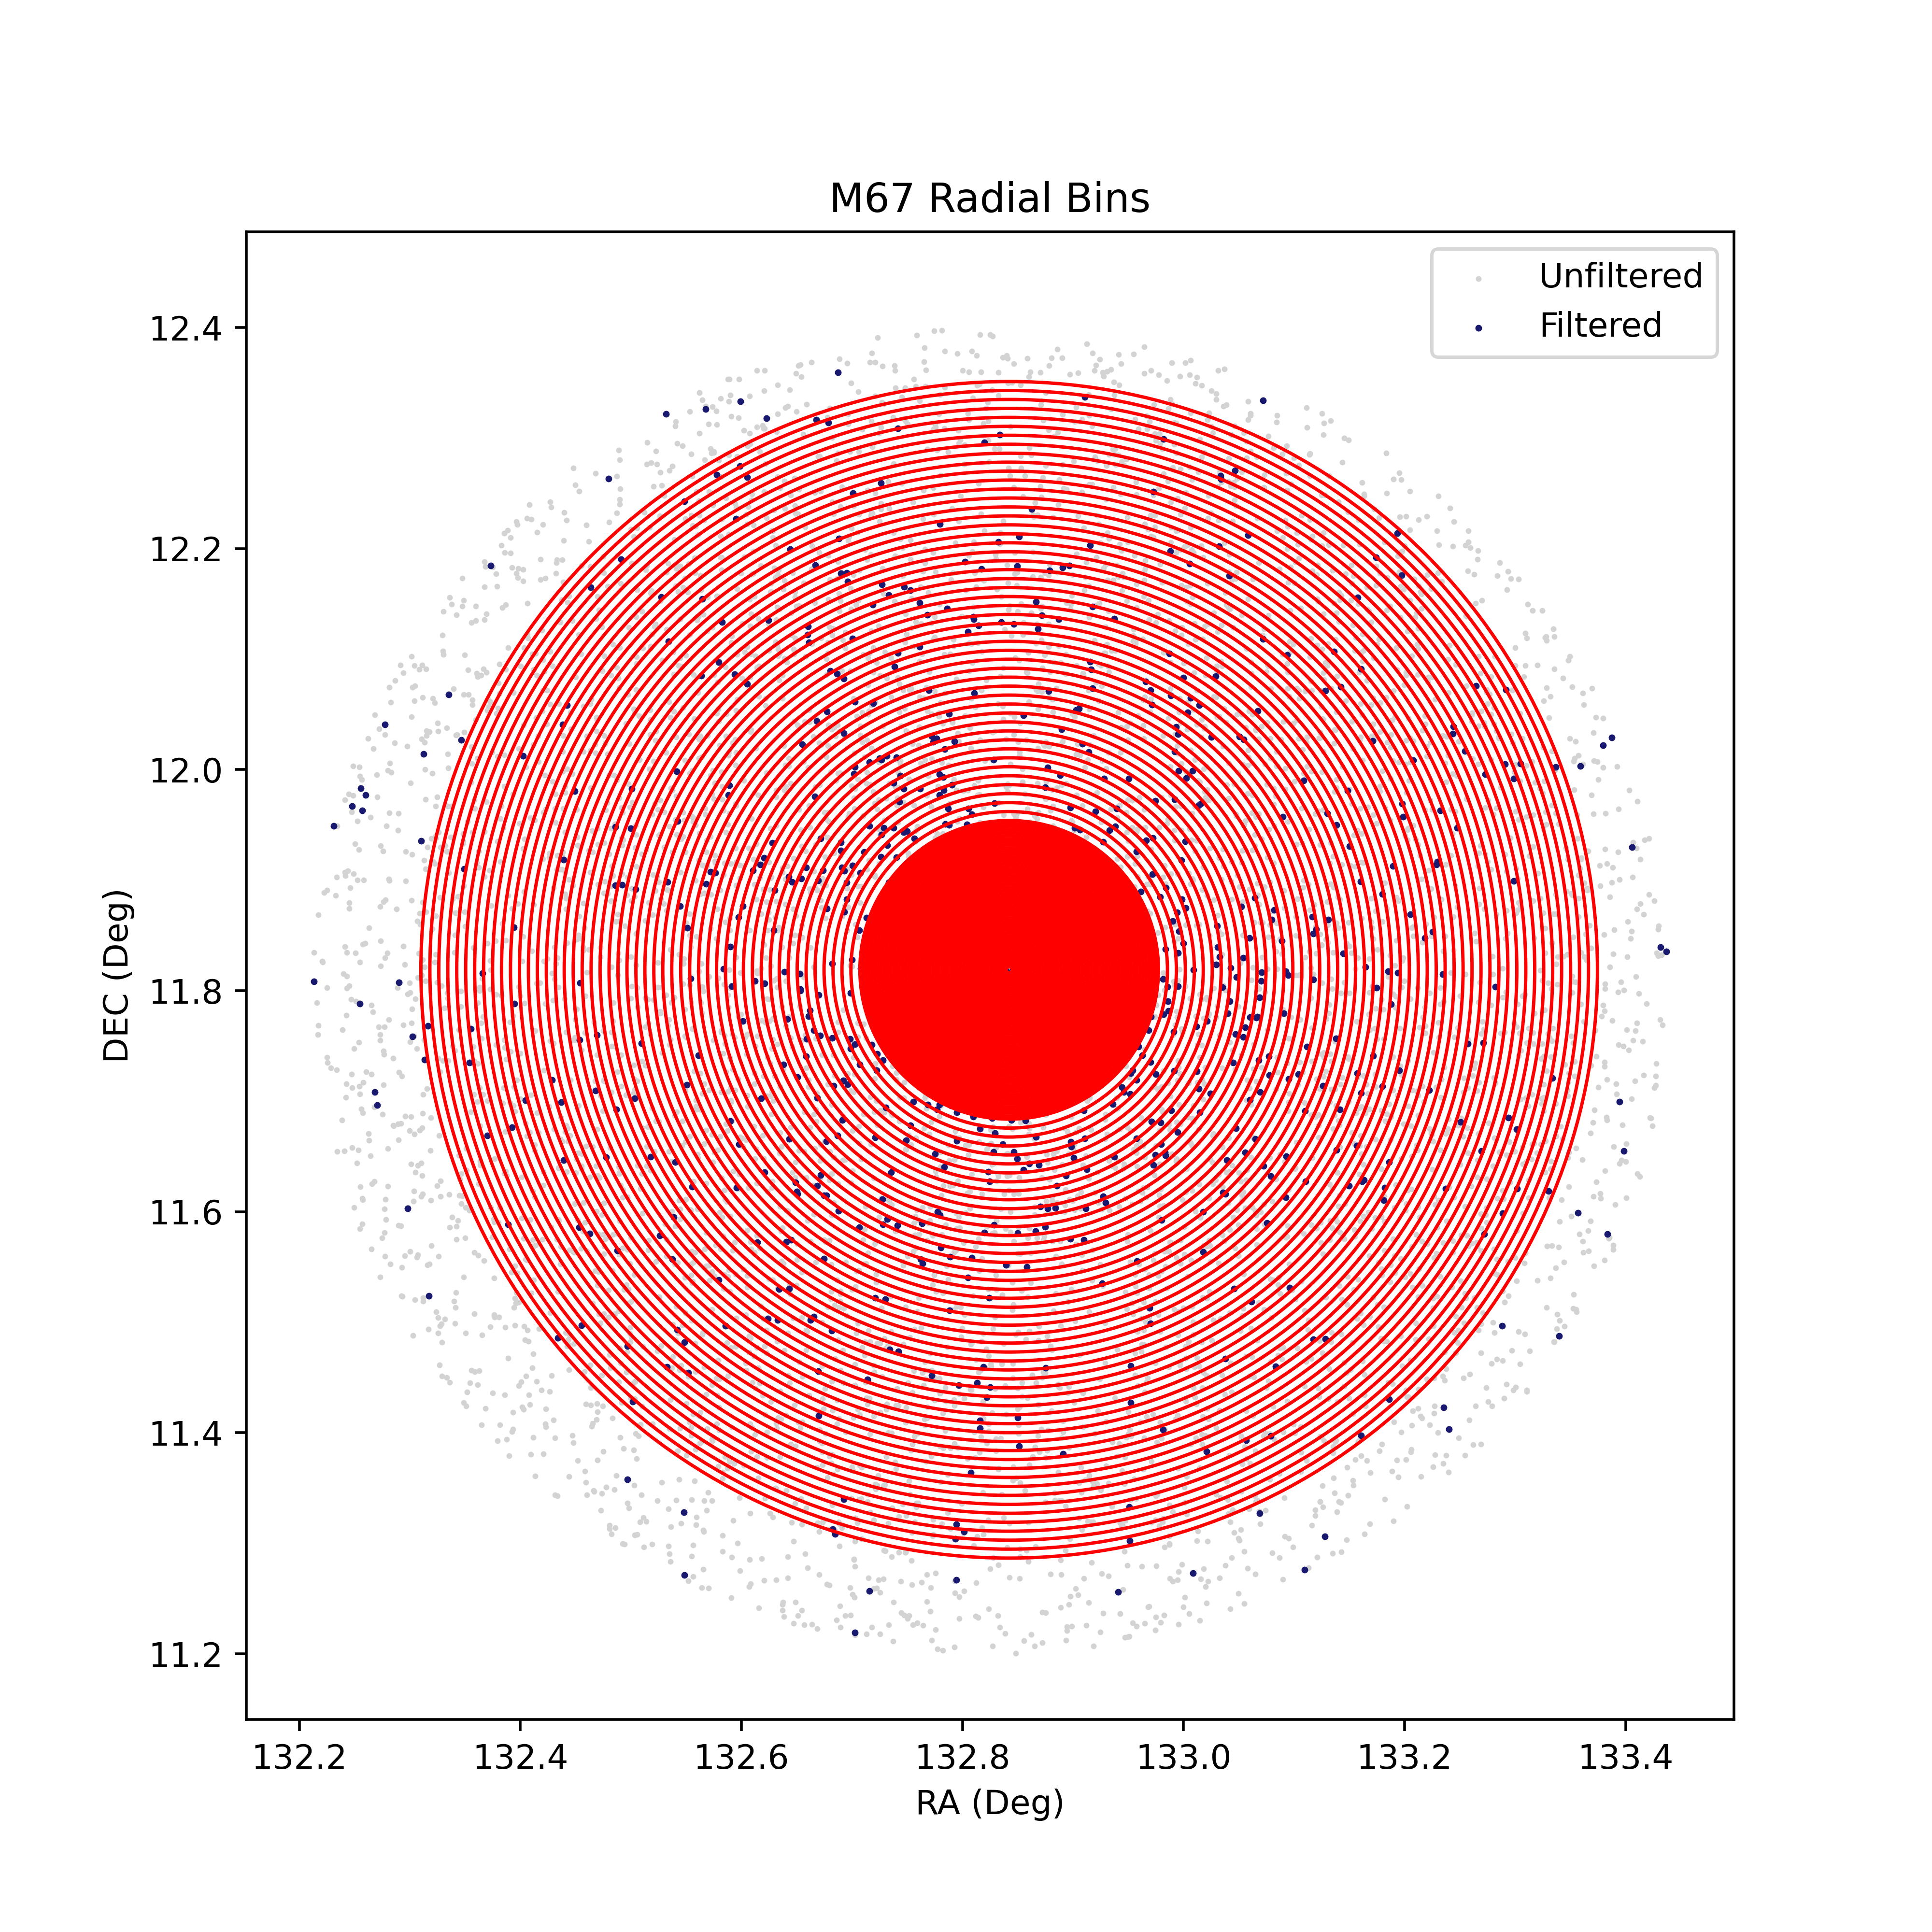
\includegraphics[width=4.75in]{figures/M67_radialBins.png}
    \caption{Demonstration of the spacing of the radial bins used in the number density and mass density calculations. The filtered and unfiltered data for Messier 67 is included for reference.}
    \label{fig:radBins}
\end{figure}

\begin{figure}[]
    \centering
      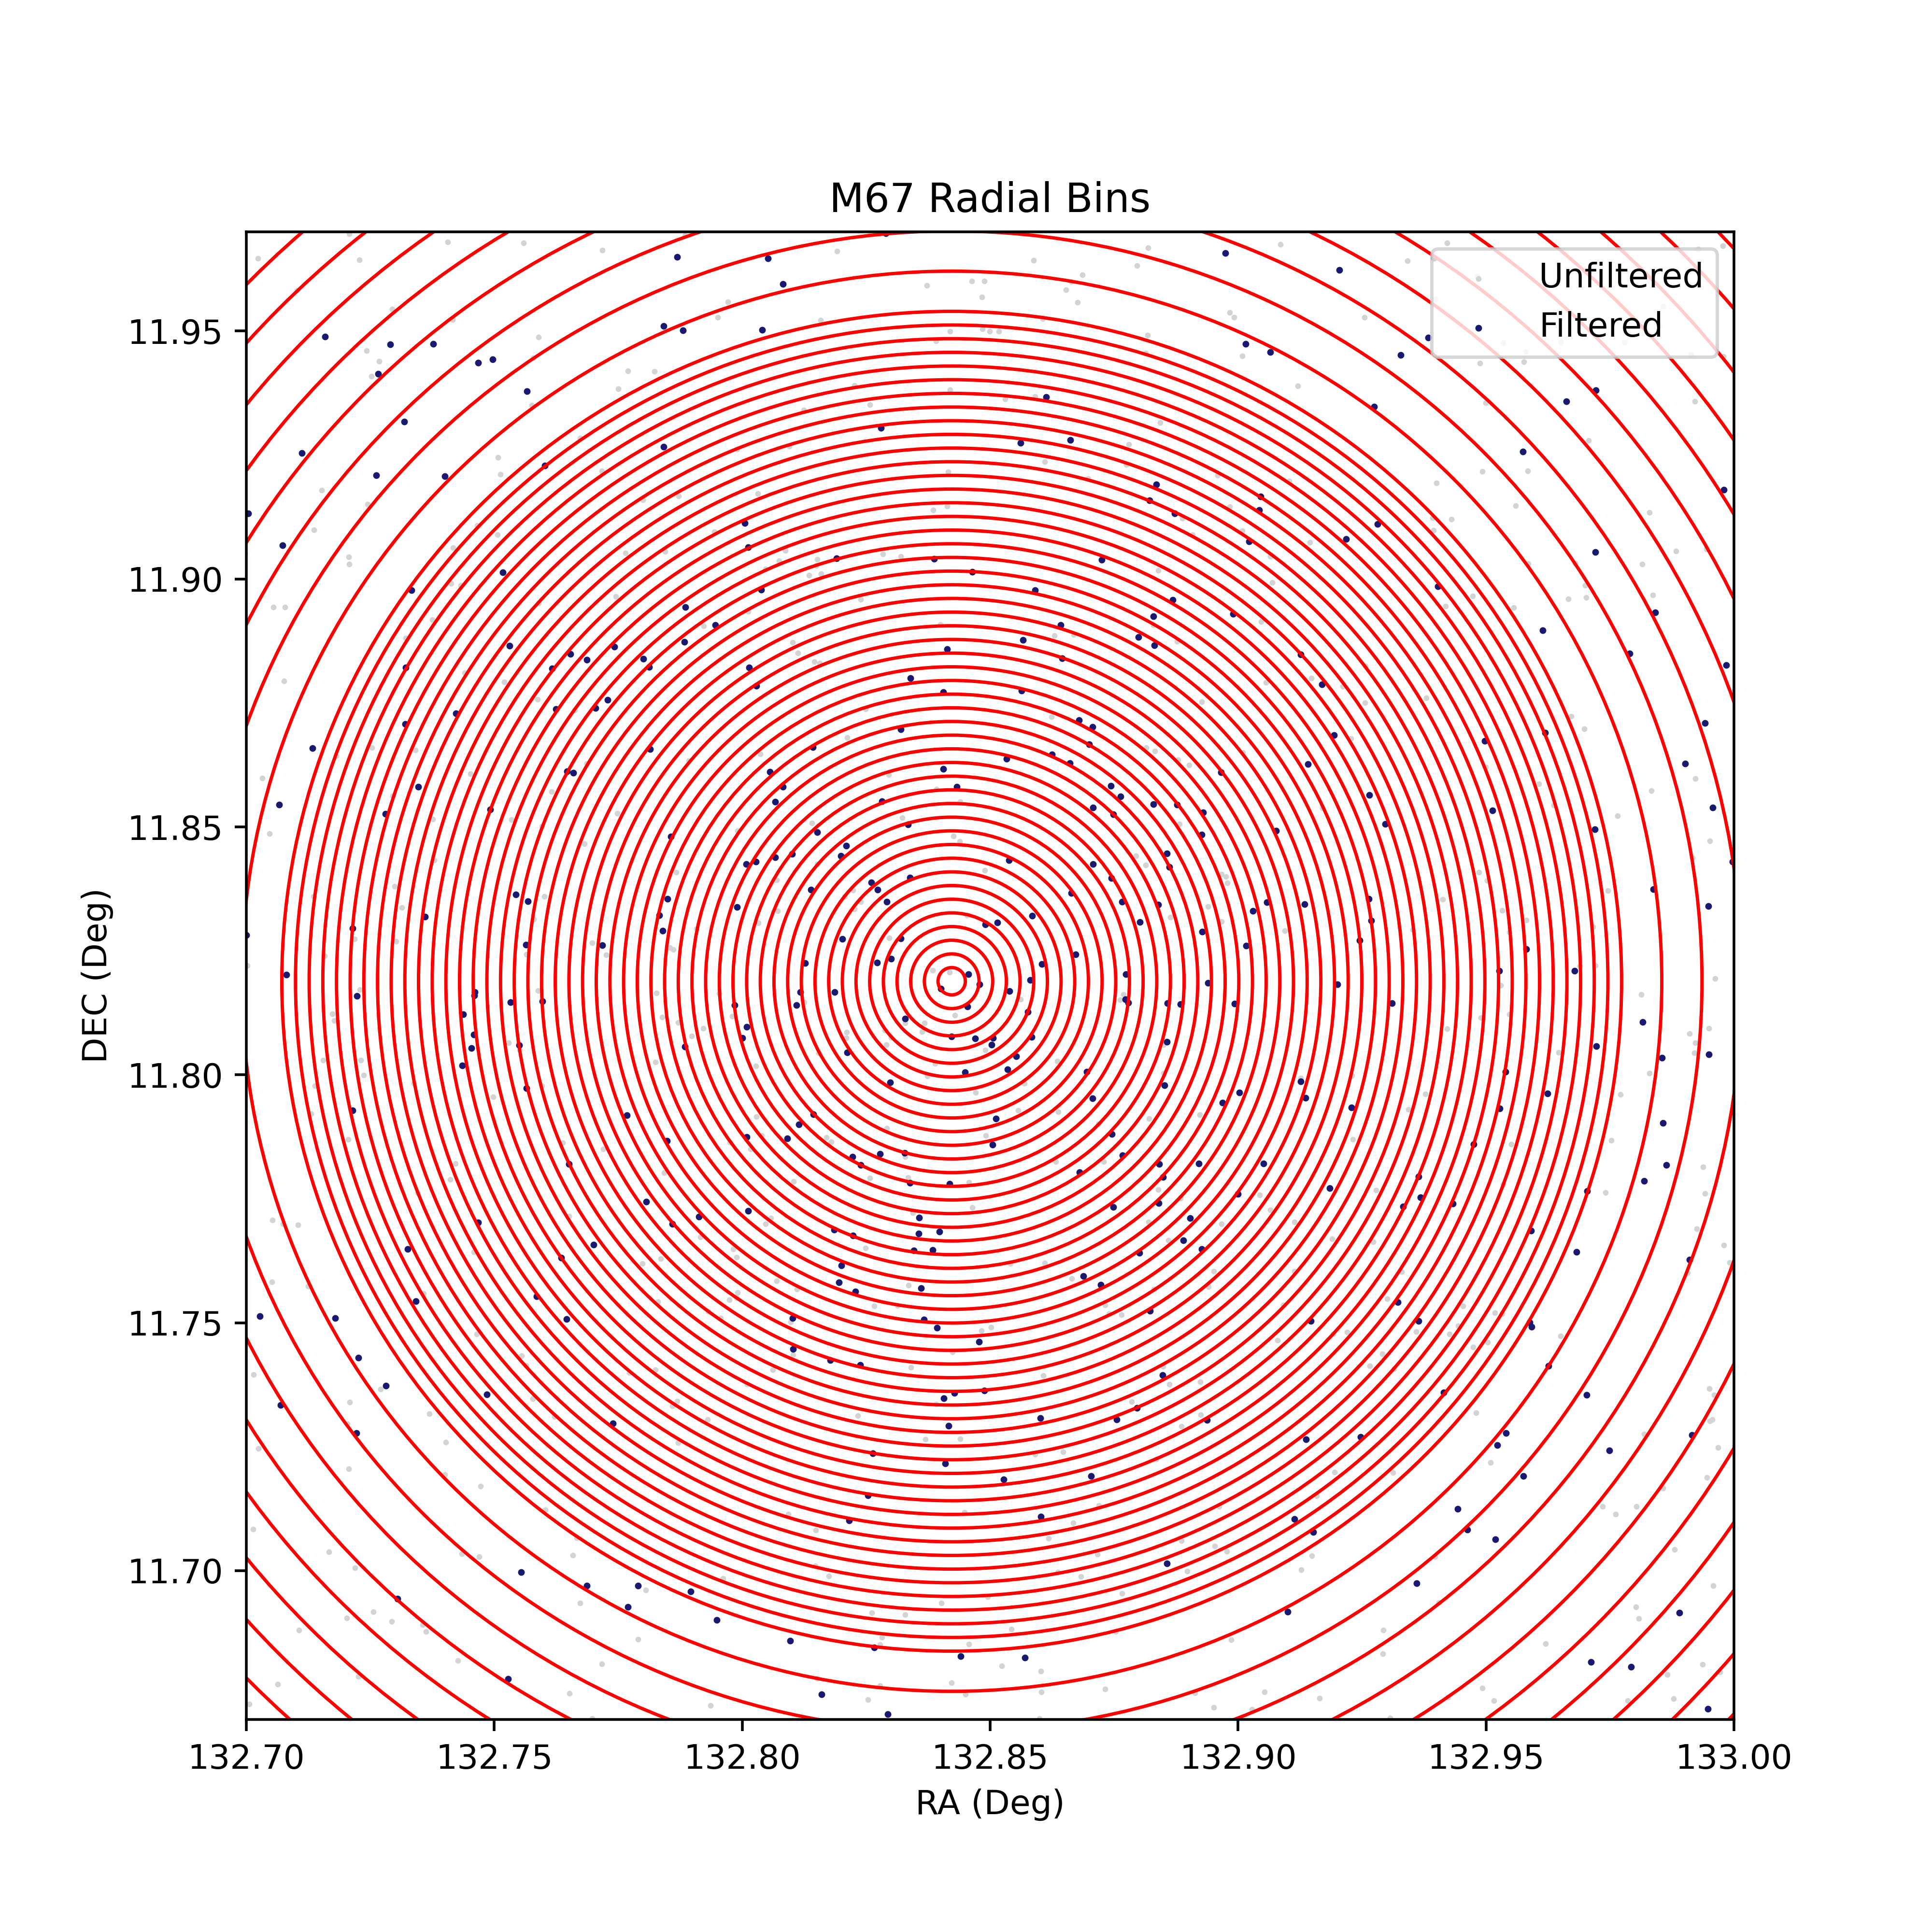
\includegraphics[width=4.75in]{figures/M67_radialBins_center.png}
    \caption{Demonstration of the spacing of the radial bins in the central region of the cluster. The inner $\frac{R}{4}$ by radius includes 50\% of the total radial bins. The innermost 5\% by radius is excluded from binning. The filtered and unfiltered data for Messier 67 is included for reference.}
    \label{fig:radBinsCenter}
\end{figure}

With radial bins selected, the number of cluster members identified in each ring is then divided by the area of the ring in square degrees to yield a surface number density. The surface number density bins are analyzed for extreme and erroneous outliers, usually manifesting as an increase or decrease between bins greater than three times that of the neighboring bins. Radial bins whose number density falls below a minimum threshold are also discarded. The result of this process is shown for example in Figure \ref{fig:M67_num_density}. In addition to the resulting surface number density in each bin, Figure \ref{fig:M67_num_density} shows the best fit density profile to the data. The shape of this profile was chosen from the spatial distribution in King 1972\protect{\cite{King_1972}}, shown in Equation \ref{eq:king}. In this model, K represents a central core density, and R represents a characteristic cluster core radius. The result of fitting this type of profile to the data is that a characteristic cluster core radius can be determined for each cluster, allowing direct quantitative comparisons of cluster size. In the past, we also attempted to fit the surface density data using an exponential decay model. This model also produced a characteristic radius for the cluster, but did not fit the surface density profiles of all clusters equally well.

\beq
\label{eq:king}
S\left(r\right) = K\left(1+\frac{r^2}{R^2}\right)^{-1}
\eeq

\begin{figure}[]
    \centering
      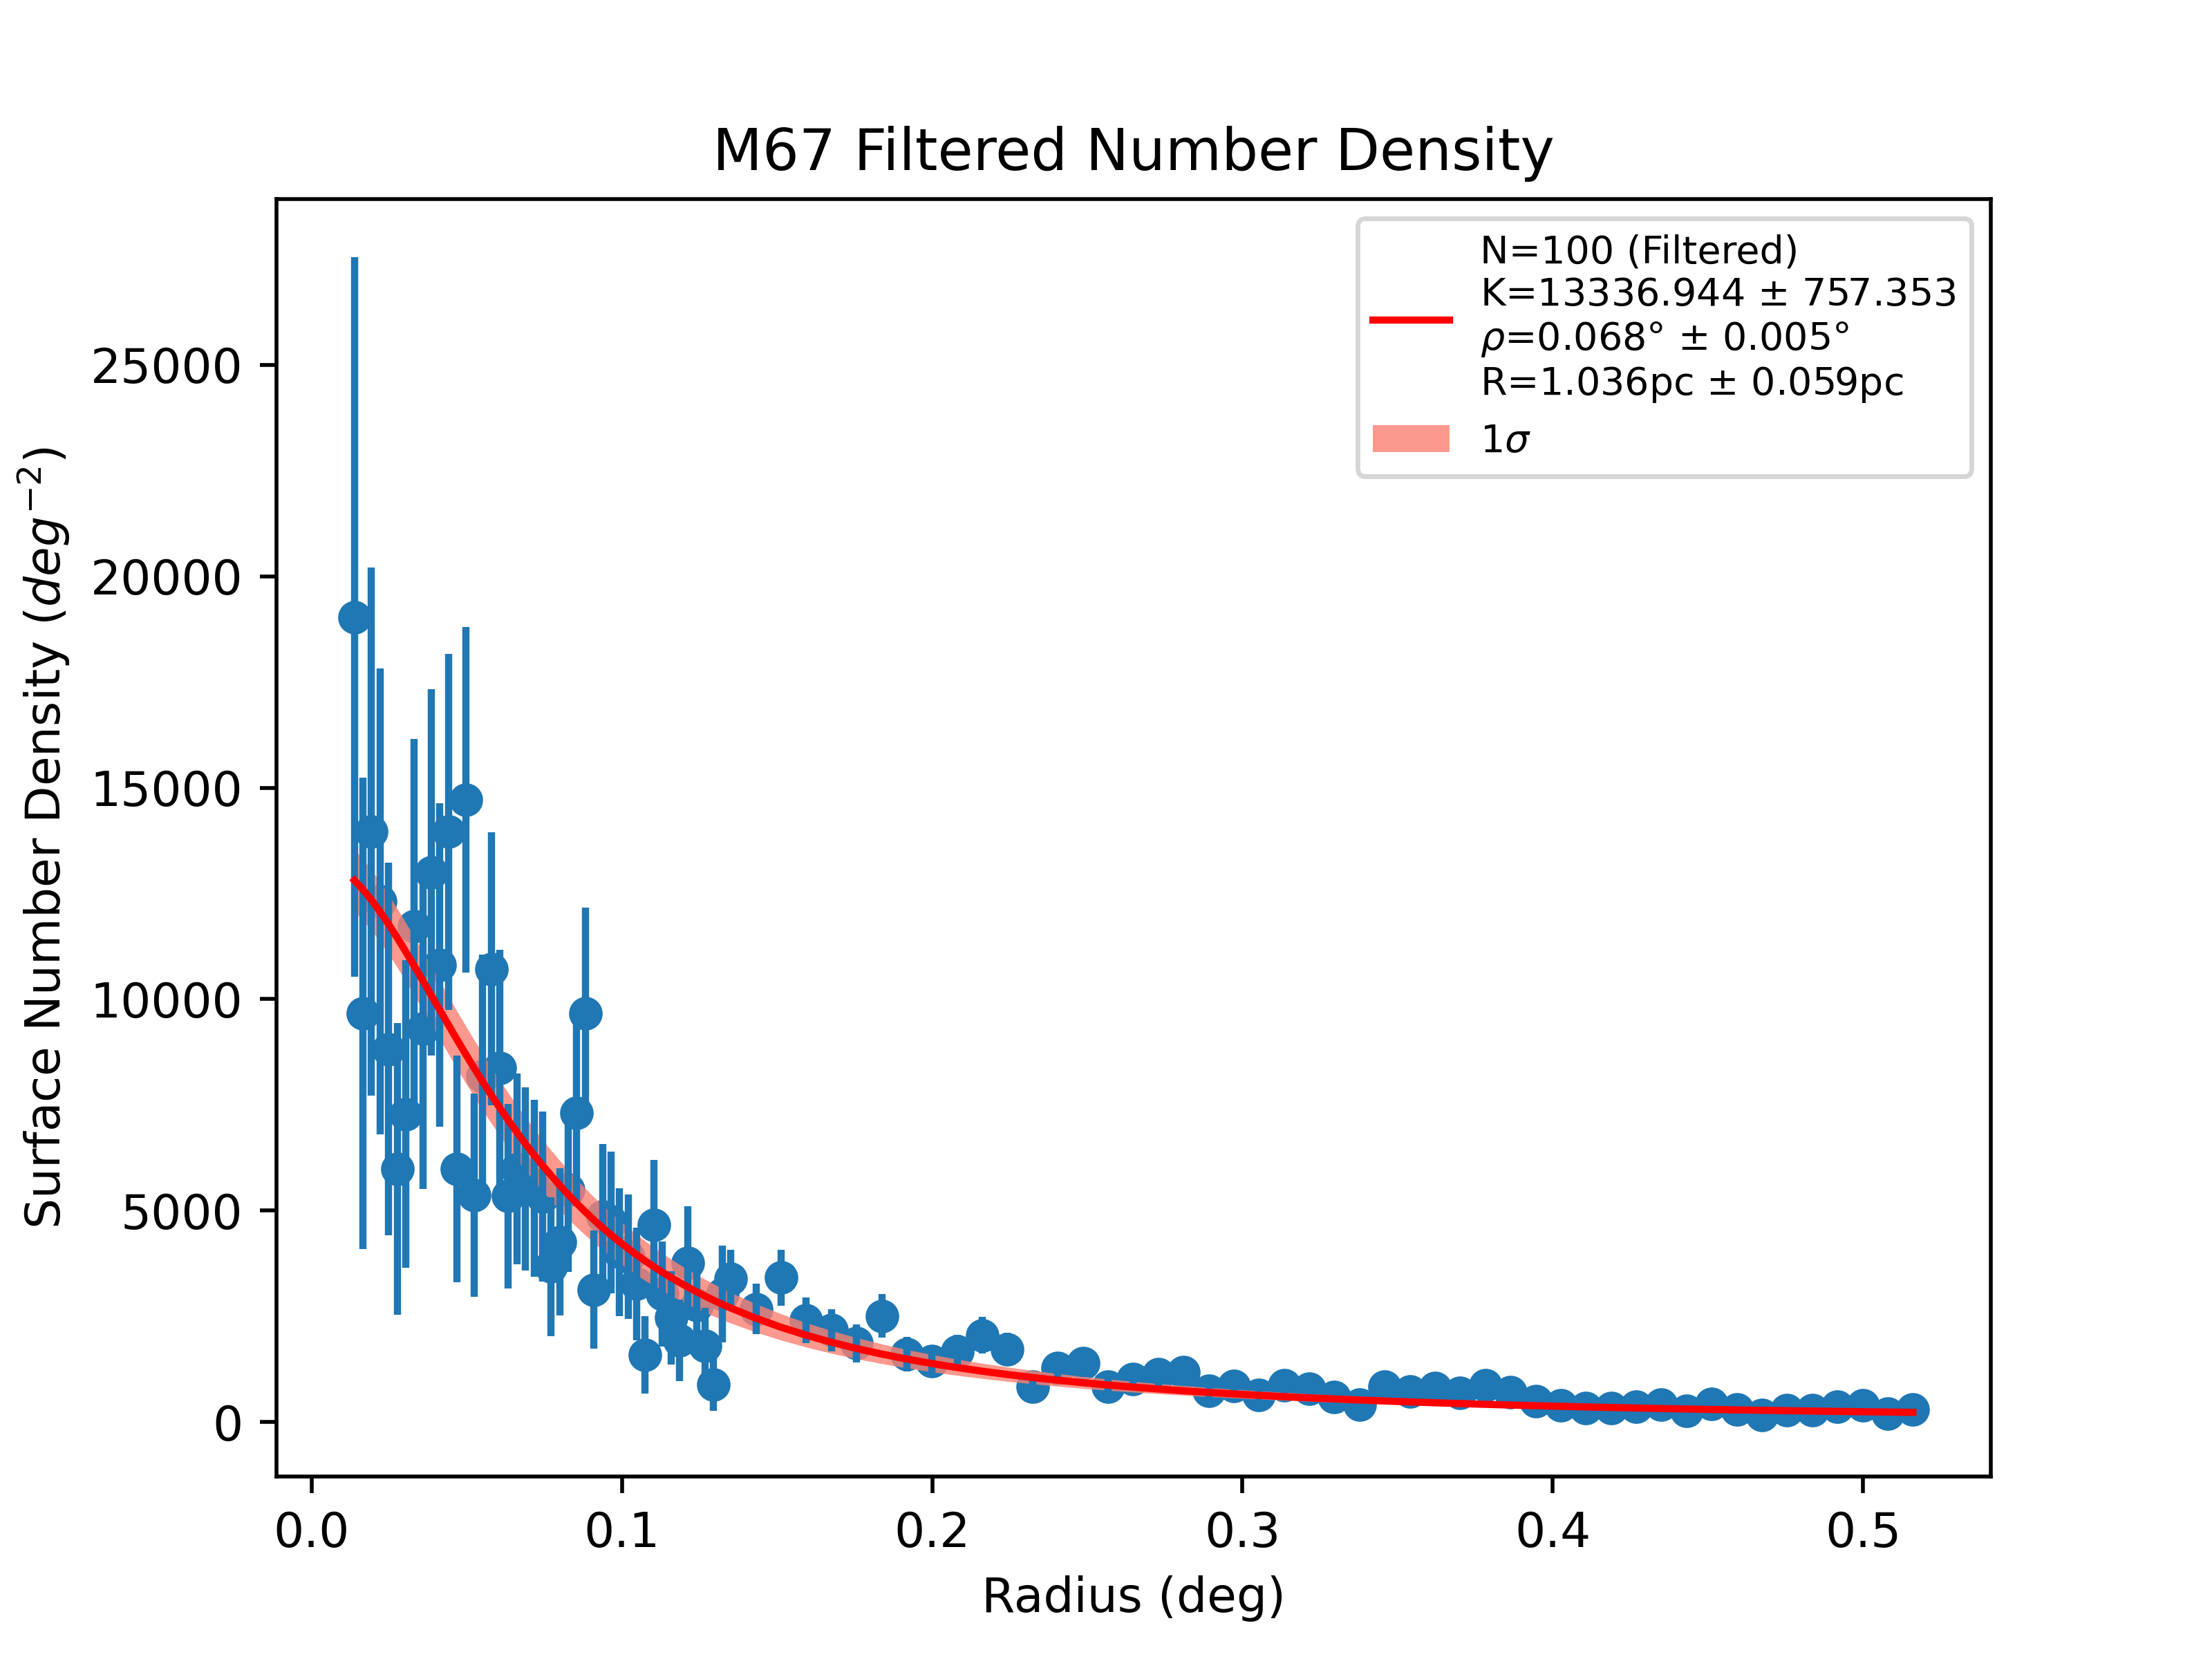
\includegraphics[width=4.75in]{figures/M67_numDensity_filtered.png}
    \caption{Surface number density for Messier 67. Calculated using 100 concentric, radial bins. The inner 25\% of the cluster by radius is sampled using 50 of those bins, with the other 75\% utilizing the other 50 bins. The fit was done using the King\protect{\cite{King_1972}} model, with $\rho$ and R representing the cluster's characteristic core radius in degrees and parsecs, respectively. The coefficient K is related to a central density, but to avoid issues related to oversampling, the inner 5\% of the cluster by radius has been omitted from the data.}
    \label{fig:M67_num_density}
\end{figure}

In addition to the surface number density, we can also visualize the surface mass density. In order to do this, we've used the mass of the nearest point on the best-fitting synthetic isochrone as a proxy mass for each real cluster member. The surface density is then calculated in the same way as in the case of number density, and an example can be seen in Figure \ref{fig:M67_mass_density}. By eye, there's little difference between the number and mass density profiles. As we might hope, the King\protect{\cite{King_1972}} profile fits for both types of density give a cluster core radius that agree within uncertainty. Across the entire sample of open clusters, there generally seems to be a slight inverse relationship between distance from the cluster center and average stellar mass at that radius. This trend is something that is further expanded upon in Section \ref{sec:pop}.

\begin{figure}[]
    \centering
      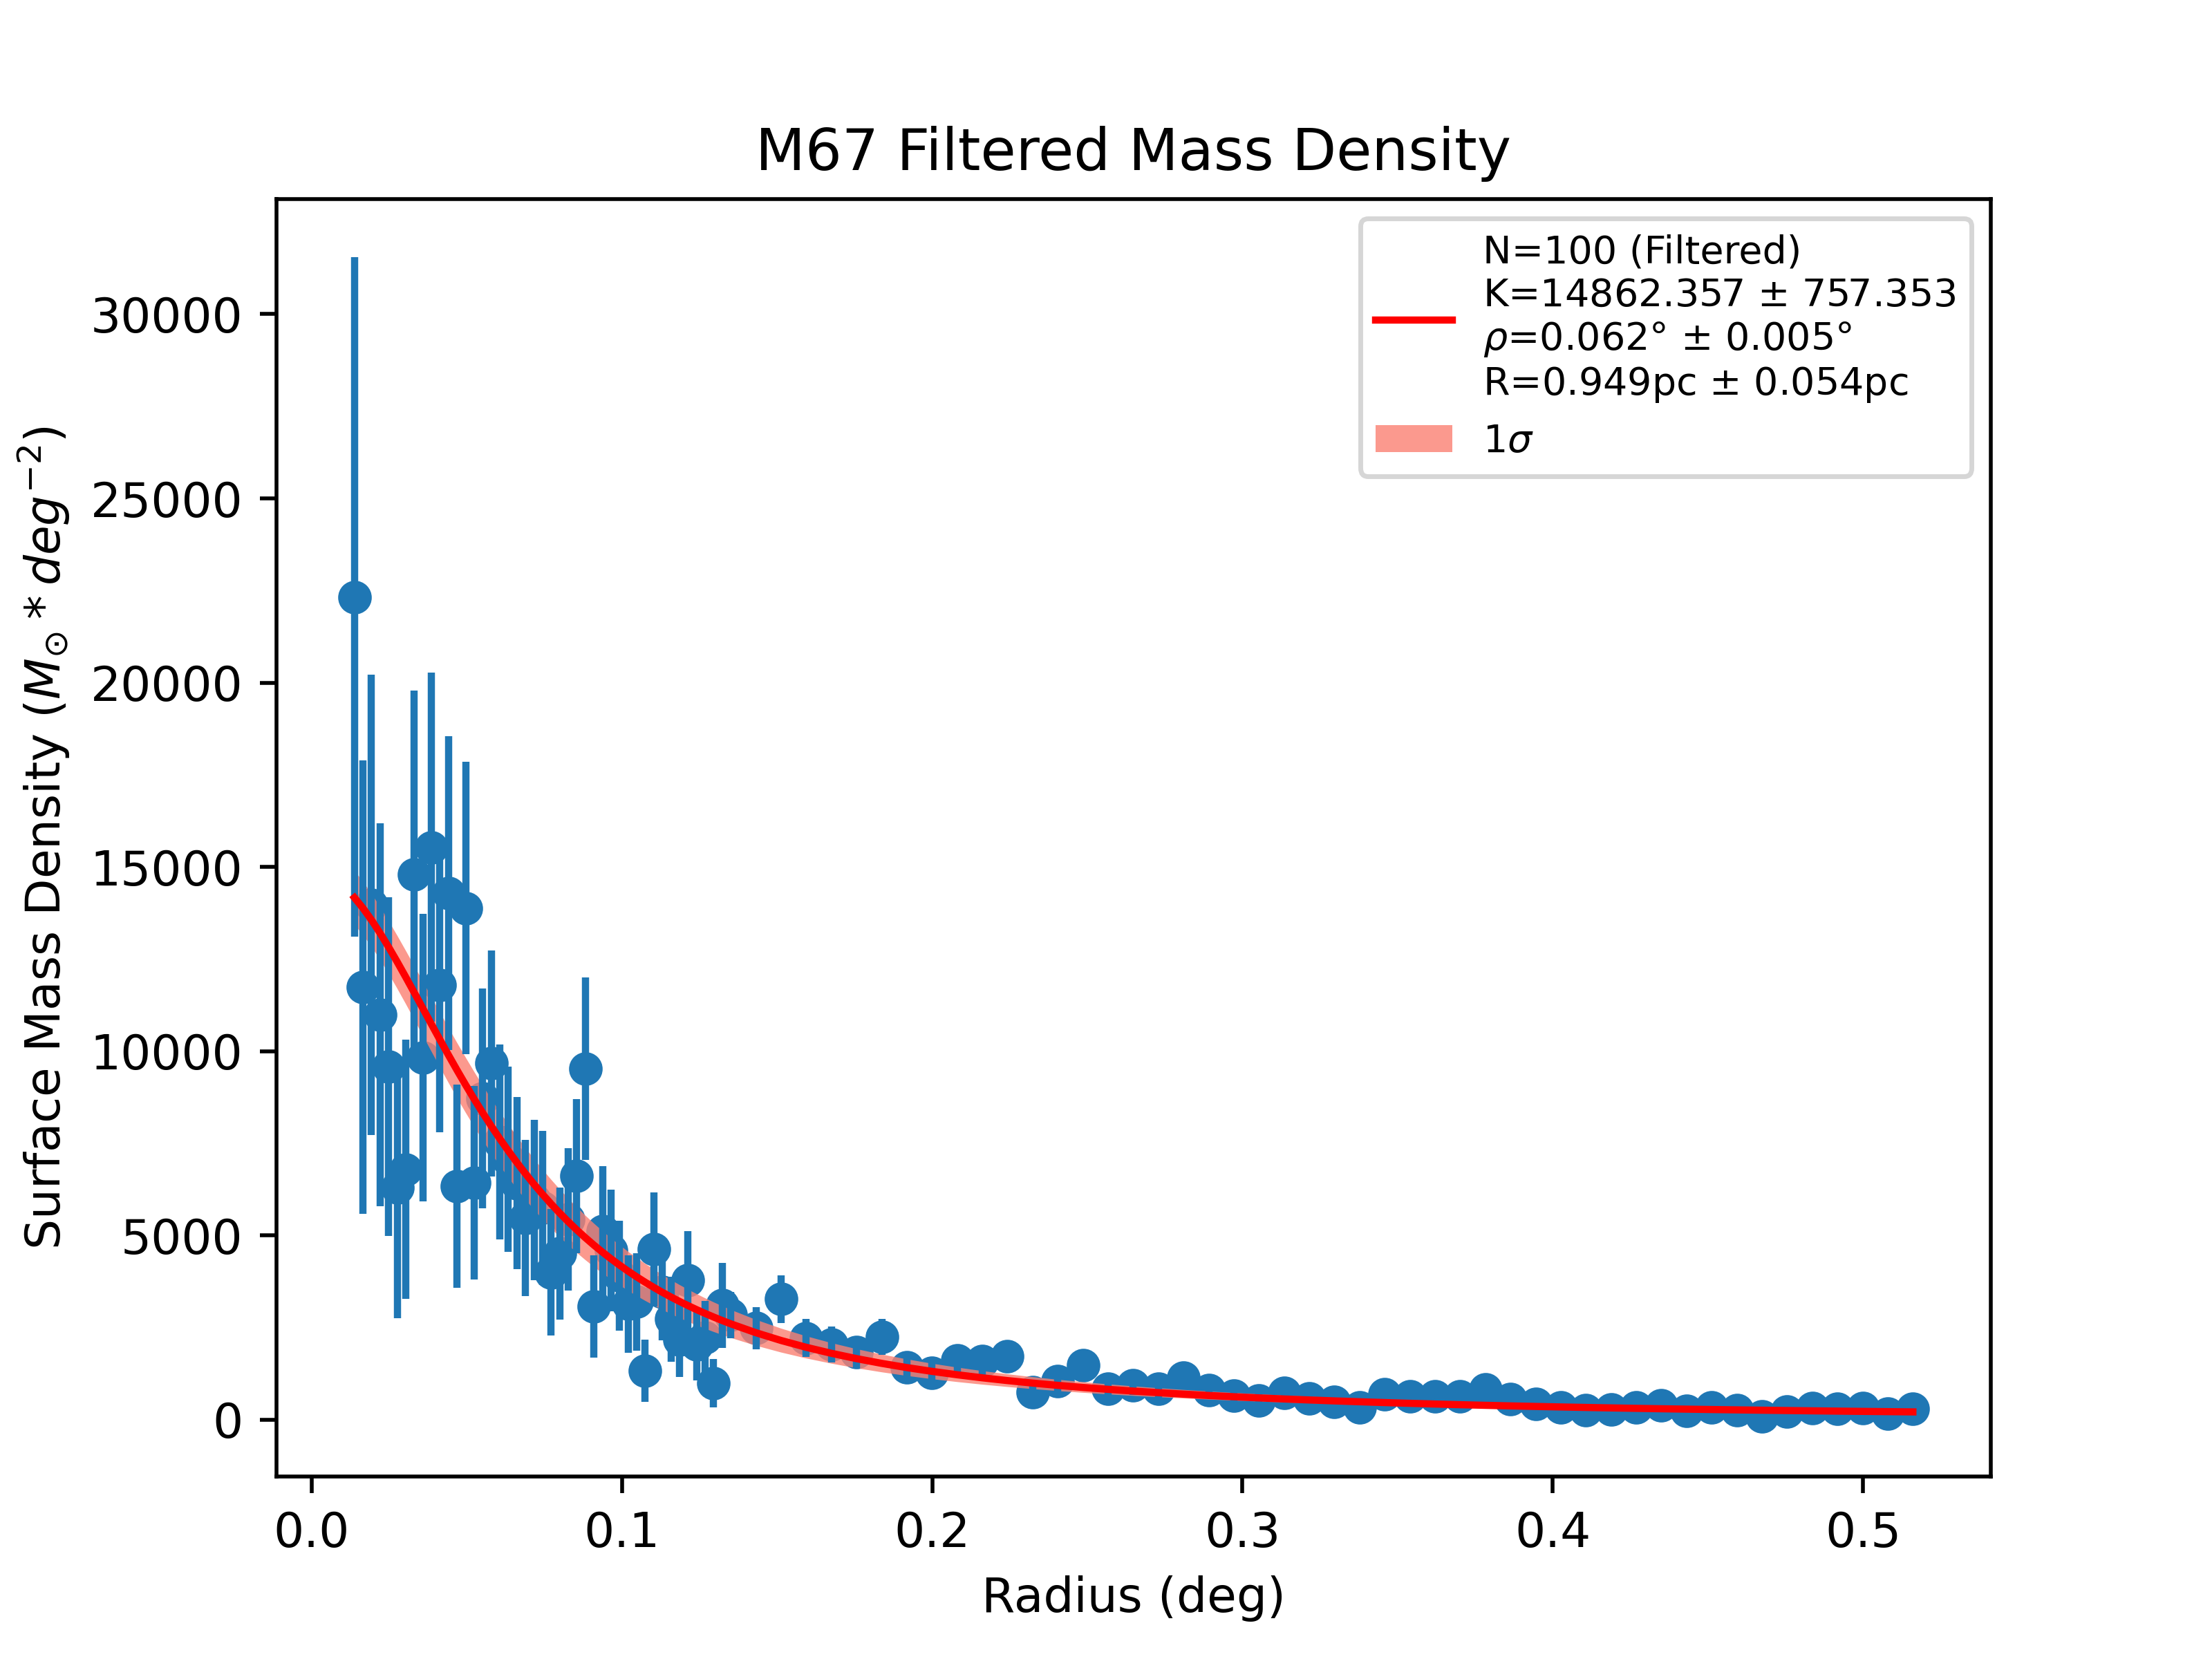
\includegraphics[width=4.75in]{figures/M67_massDensity_filtered.png}
    \caption{Surface mass density for Messier 67. Calculated in the same way as Figure \ref{fig:M67_num_density}, and using the proxy mass values from the nearest synthetic isochrone star to each observed cluster member. The characteristic core radius determined by the King\protect{\cite{King_1972}} fit is in agreement with that of the number density plot, within one standard deviation.}
    \label{fig:M67_mass_density}
\end{figure}

As an additional analysis to each cluster's mass distribution, we look at the average mass of each cluster member as a function of distance from the cluster center. We calculate this by dividing the calculated mass densities by the number densities in each radial bin. The average mass values for each bin, shown in blue in Figure \ref{fig:M67_average_mass}, are separated into 5 broad bins, each representing 20\% of the cluster by radius. In each of the broad bins, we determine an interquartile mean, shown as red points in the figure. The interquartile mean takes the mean over the 25th percentile to the 75th percentile of the measurements in an effort to be more robust of a statistic against influence from outliers. The red line seen in Figure \ref{fig:M67_average_mass} shows a linear fit to the interquartile mean values, the slope of which gives an estimate for the linear mass drop-off in each cluster. In most clusters, this mass drop-off is of order 0.1 solar masses over the entire cluster radius. Finally, we created histograms for the population statistics in each cluster by mass, de-reddened color index, and corrected, absolute G-band magnitude. While we were unable to draw conclusive trends between clusters from these histograms, we leave Figures \ref{fig:M67_mass_hist}, \ref{fig:M67_mag_hist}, and \ref{fig:M67_color_hist} as examples. Finally, we determine other characteristic core radii for each cluster to compare to that from the King profile fit. Table \ref{tab:radii} summarizes the relevant distances and radii for all 16 open clusters, including the half light and half mass radii.

\begin{table}[!h]
\centering
\rowcolors{2}{white}{gray!25}
\begin{tabular}{lllllll}
\toprule
Cluster &
  \begin{tabular}[c]{@{}l@{}}Distance  from\\ Observer (pc)\end{tabular} &
  \begin{tabular}[c]{@{}l@{}}Dist. from Gal. \\ Center (pc)\end{tabular} &
  \begin{tabular}[c]{@{}l@{}}King Profile\\ Radius (pc)\end{tabular} &
  \begin{tabular}[c]{@{}l@{}}Half Light\\ Radius (pc)\end{tabular} &
  \begin{tabular}[c]{@{}l@{}}Half Mass\\ Radius (pc)\end{tabular} &
  \begin{tabular}[c]{@{}l@{}}Median Star\\ Radius (pc)\end{tabular} \\ \midrule
IC4651  & 943  & 7121  & 1.81 & 1.91 & 3.89  & 4.24 \\
M35     & 871  & 8866  & 2.43 & 3.03 & 4.51  & 4.70 \\
M46     & 1668 & 9124  & 3.64 & 4.95 & 6.26  & 6.70 \\
M47     & 479  & 8310  & 1.16 & 1.02 & 1.83  & 2.21 \\
M48     & 759  & 8528  & 1.71 & 2.71 & 4.27  & 4.85 \\
M50     & 973  & 8751  & 1.77 & 3.06 & 4.10  & 4.62 \\
M67     & 873  & 8724  & 1.04 & 2.81 & 3.03  & 3.27 \\
NGC188  & 1940 & 9198  & 2.15 & 4.83 & 4.27  & 4.36  \\
NGC2158 & 4659 & 12639 & 3.11 & 5.22 & 5.98  & 6.55 \\
NGC2204 & 4896 & 11932 & 3.78 & 9.04 & 9.34  & 9.37 \\
NGC2301 & 889  & 8762  & 1.41 & 3.59 & 3.35  & 3.59 \\
NGC2355 & 1942 & 9813  & 1.23 & 1.62 & 3.71  & 4.01 \\
NGC2360 & 1121 & 8766  & 1.53 & 2.34 & 3.68  & 4.02 \\
NGC6633 & 381  & 7696  & 1.09 & 2.27 & 2.36  & 2.48 \\
NGC6791 & 4140 & 7645  & 2.85 & 6.19 & 6.31  & 6.36 \\
NGC752  & 443  & 8329  & 0.53 & 3.01 & 3.18  & 3.22 \\ \bottomrule
\end{tabular}
\caption{Summary of the relevant distances and radii for each of the 16 open clusters studied in this work. Distance from the galactic center was calculated using parallax-distance to the object and an assumed 8000 parsecs from the observer to the galactic center. The King profile radius reported is determined from the number density profile. All numbers shown are calculated from the filtered list of cluster members, without a color index limit enforced. The listed radii for NGC 188 were calculated using a normalized RA$\cdot$cos(Dec) in place of right ascension, to counteract the effects of RA distortion at high declination.}
\label{tab:radii}
\end{table}

\begin{figure}[]
    \centering
      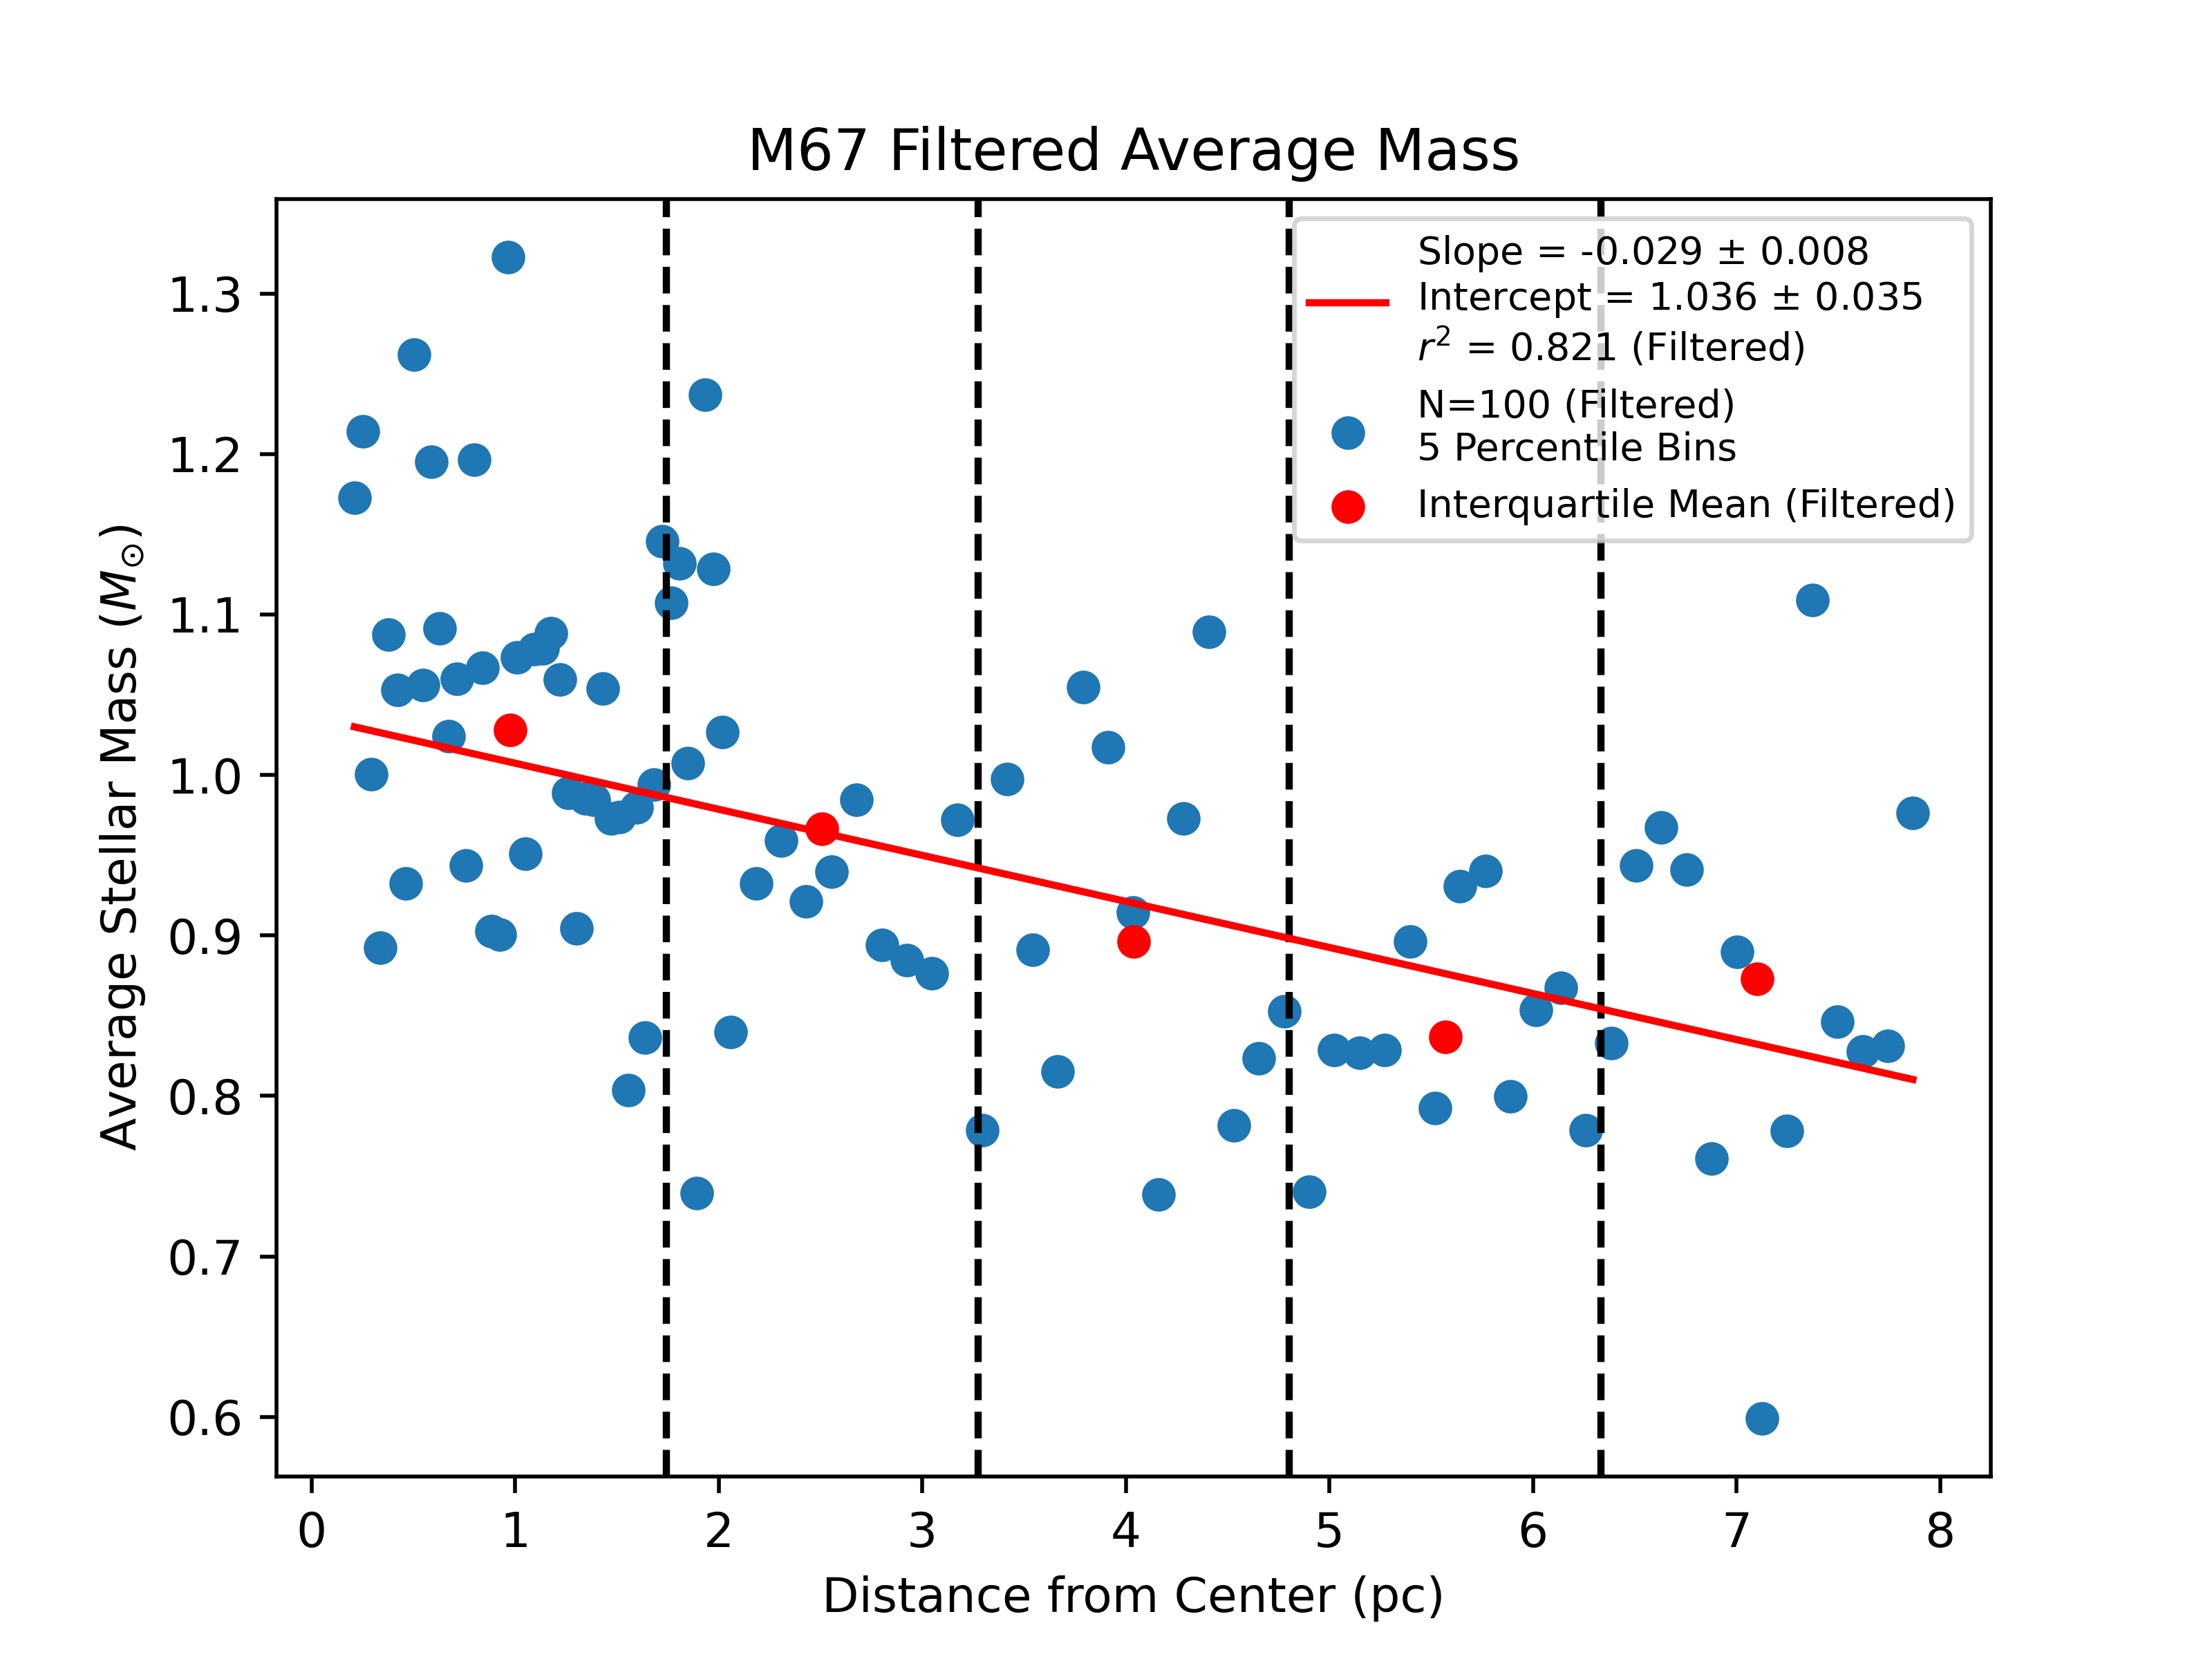
\includegraphics[width=4.75in]{figures/M67_averageMass_filtered.png}
    \caption{Average stellar mass for members of Messier 67 as a function of distance from the center in parsecs. The blue points were found by dividing the mass density by the number density, thus giving an average mass. The red points identify an interquartile mean of the blue points in each bin, i.e. the mean of the points from the 25th to 75th percentile in each bin. The red line represents a linear fit to the interquartile means, with a slope that reflects the change in mass as a function of position in the cluster and an intercept representing the average stellar mass in the cluster core.}
    \label{fig:M67_average_mass}
\end{figure}

\begin{figure}[]
    \centering
      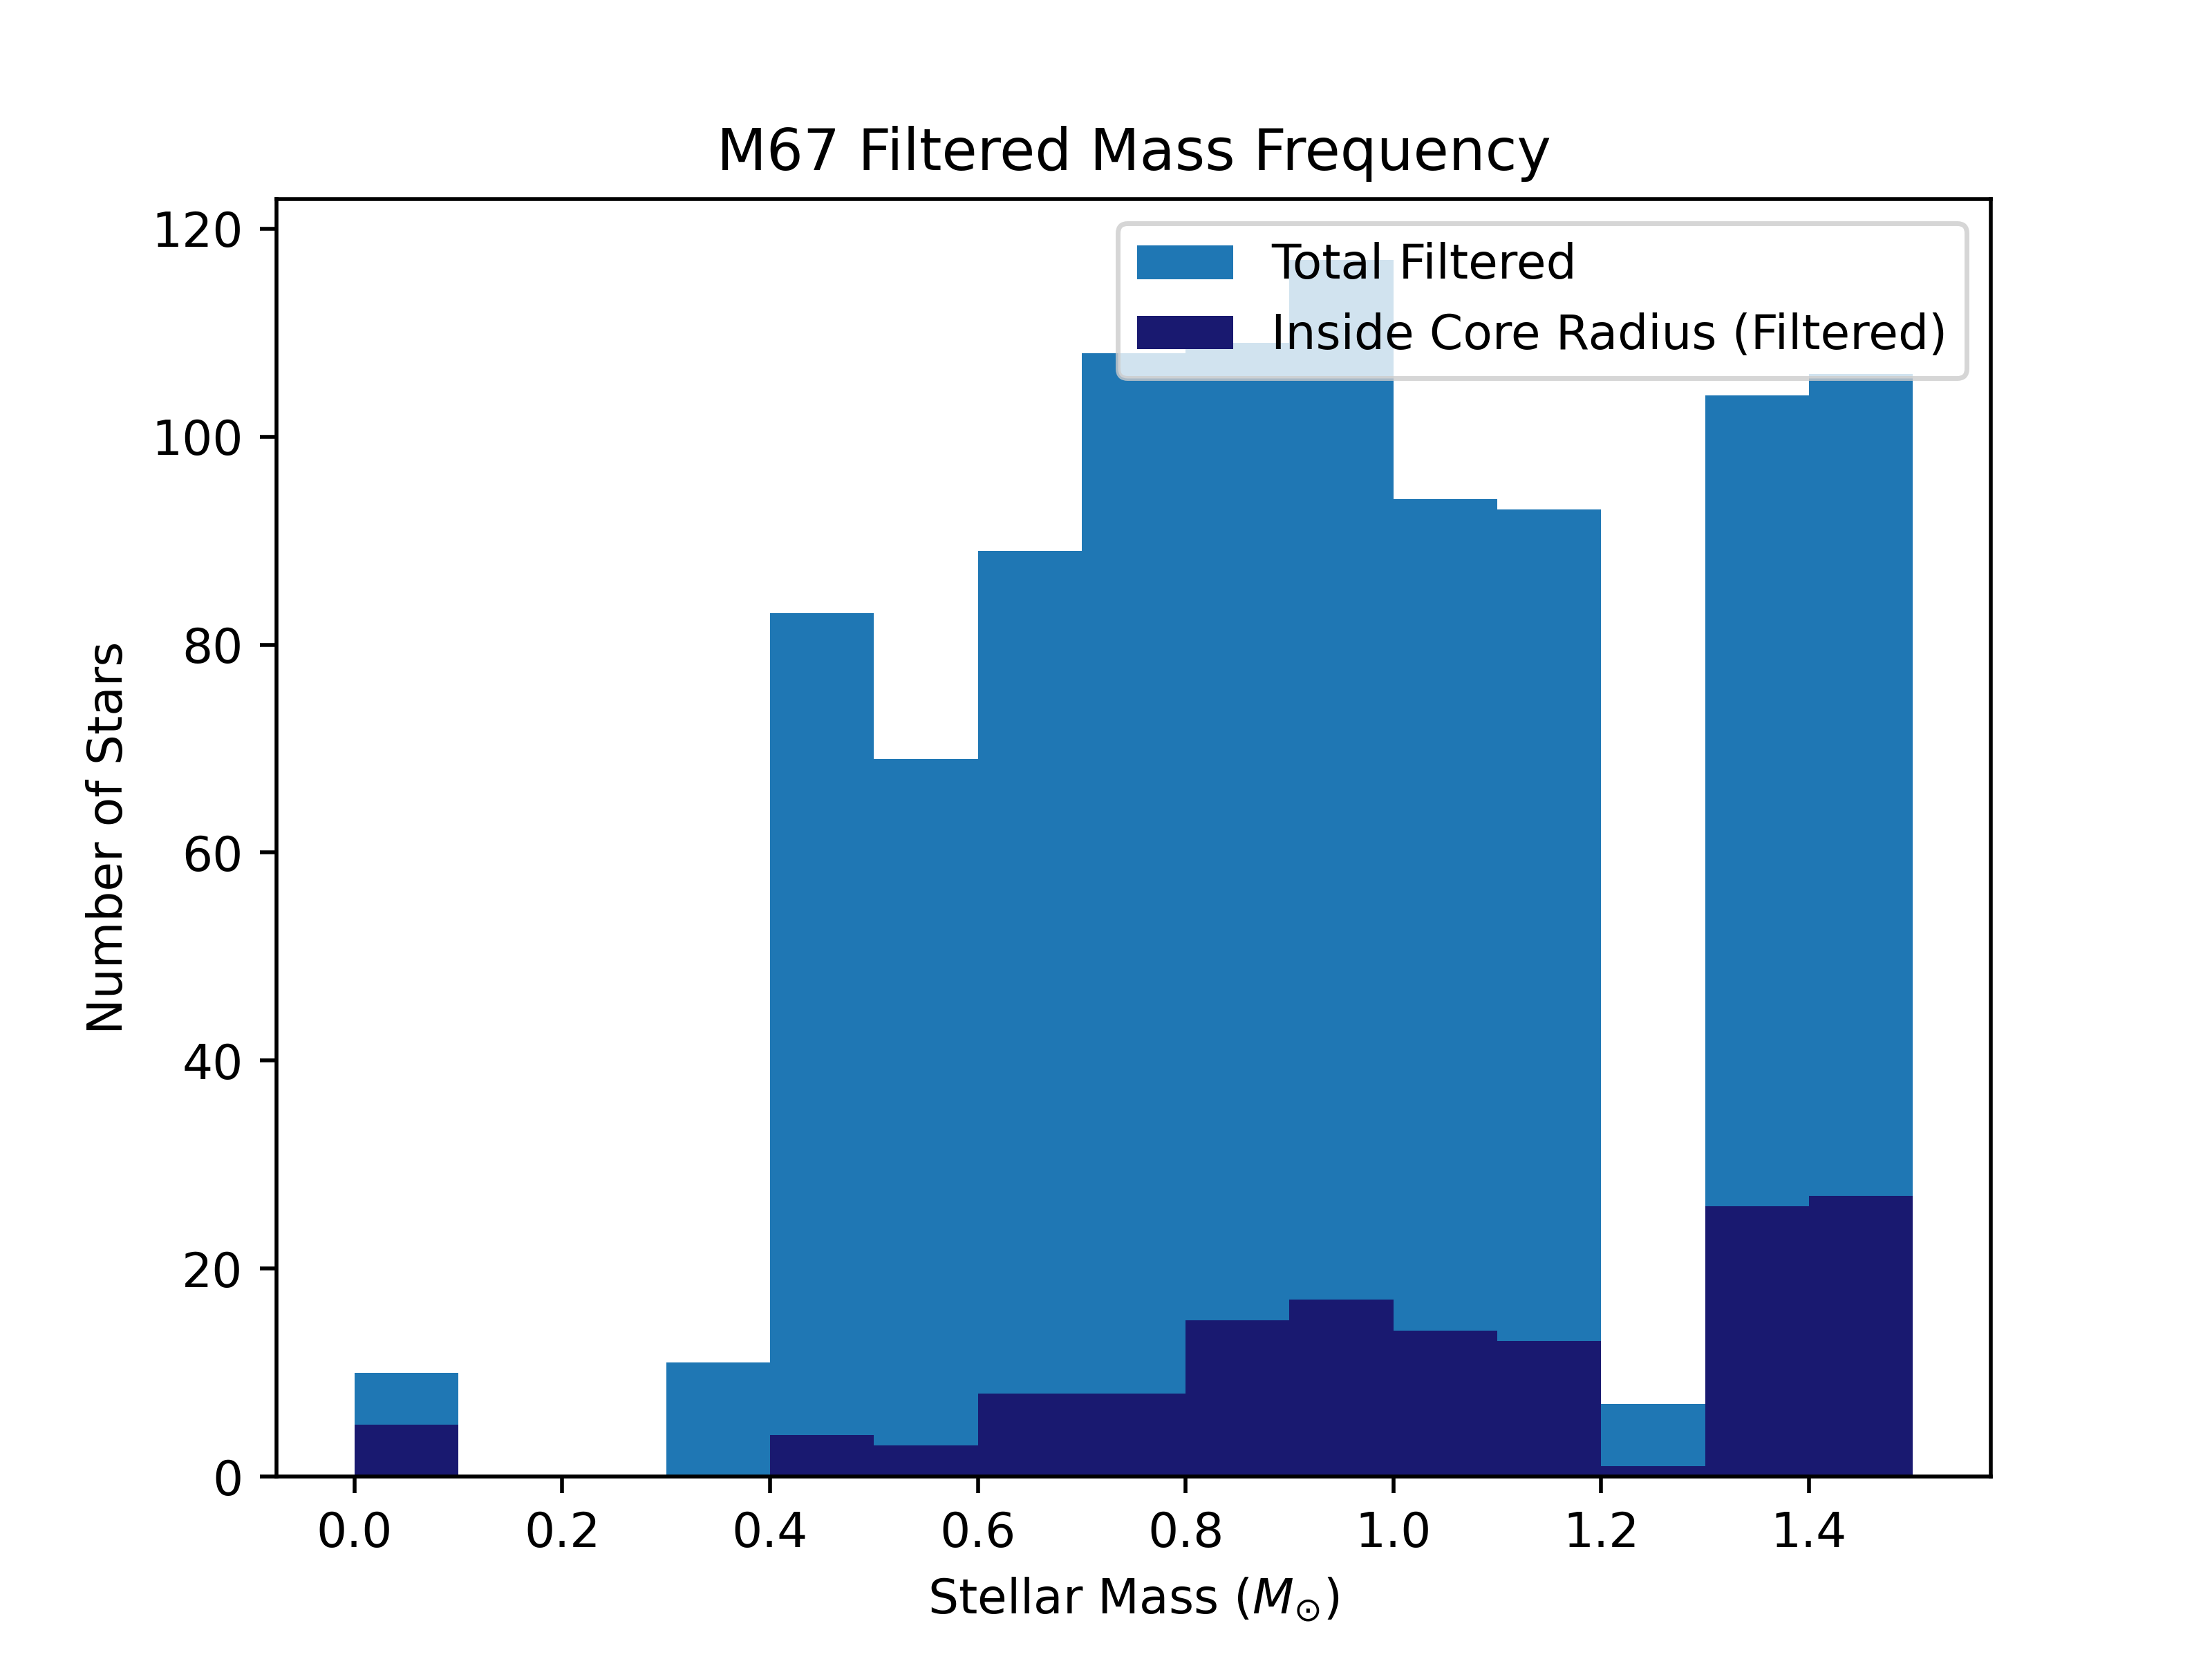
\includegraphics[width=4.75in]{figures/M67_massFrequency_filtered.png}
    \caption{Histogram of the stellar mass of cluster members belonging to Messier 67. Dark blue tracks the stars interior to the cluster core radius, determined by fitting a profile to the number density.}
    \label{fig:M67_mass_hist}
\end{figure}

\begin{figure}[]
    \centering
      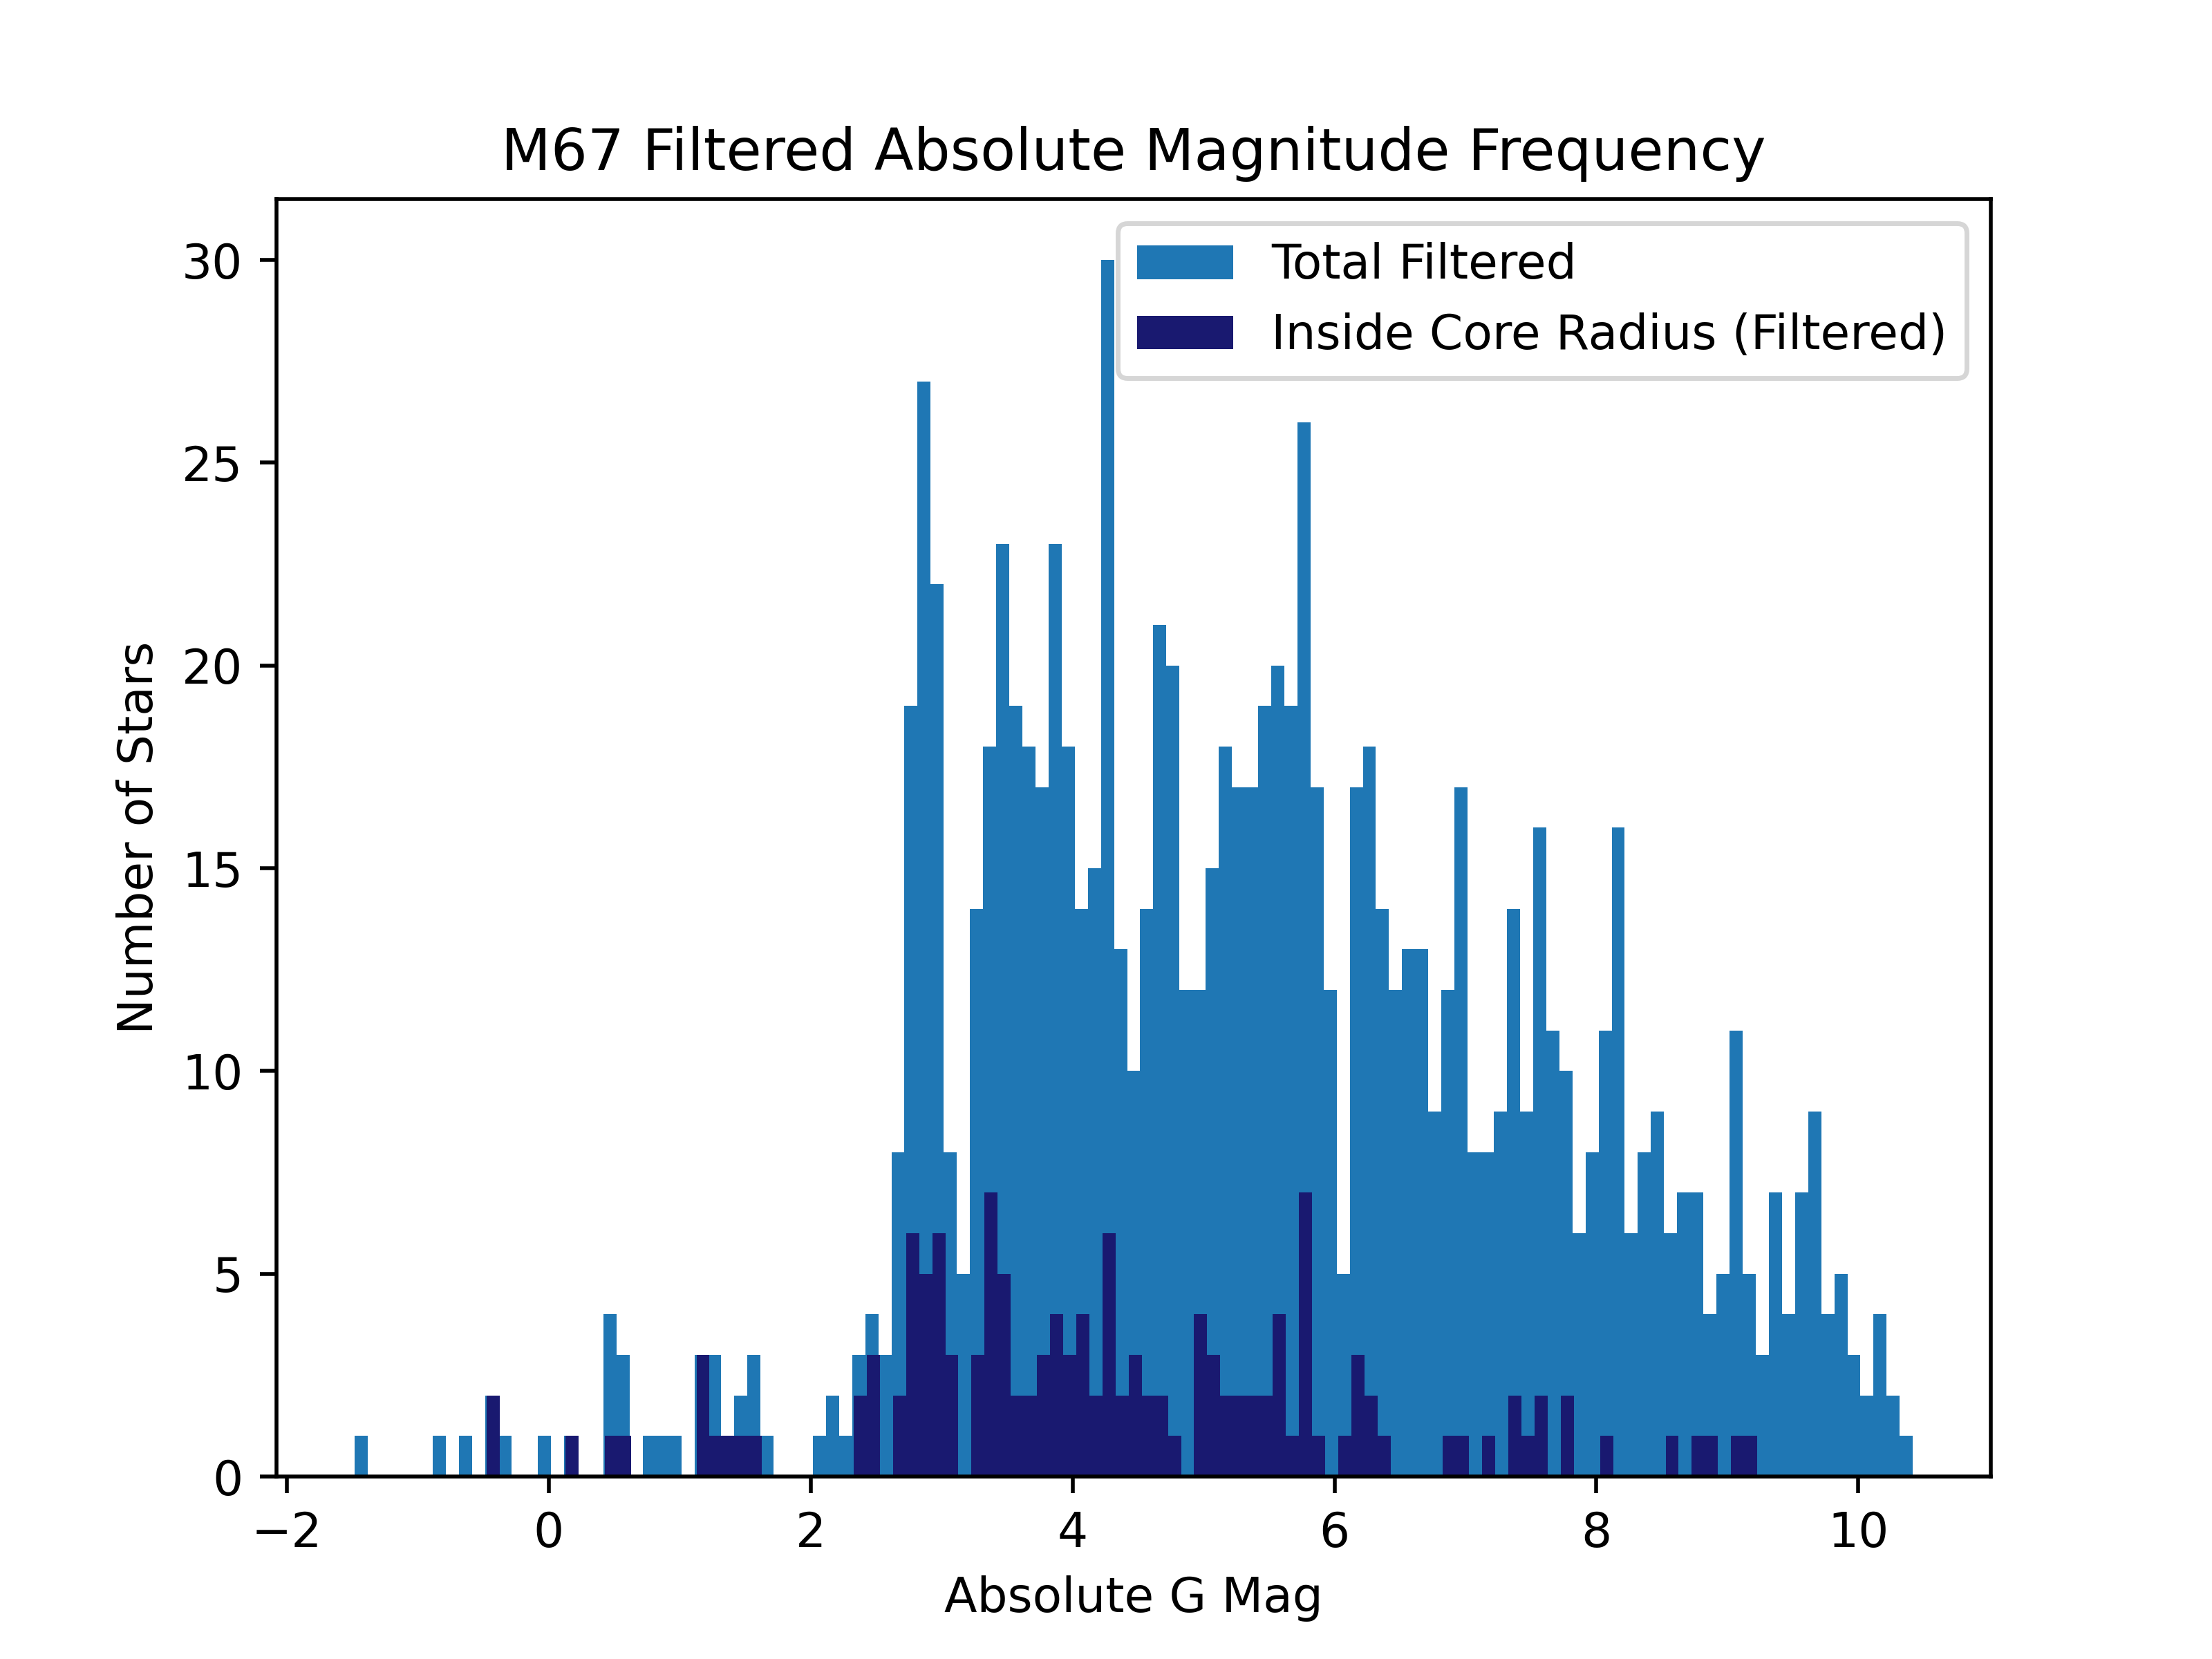
\includegraphics[width=4.75in]{figures/M67_magFrequency_filtered.png}
    \caption{Histogram of the corrected, absolute G-band magnitude of cluster members belonging to Messier 67. Dark blue tracks the stars interior to the cluster core radius, determined by fitting a profile to the number density. We deferred the choice of bin size to Pyplot's algorithm for automatically determining the number and size of bins, though one could argue that some effects of over-binning are visible here.}
    \label{fig:M67_mag_hist}
\end{figure}

\begin{figure}[]
    \centering
      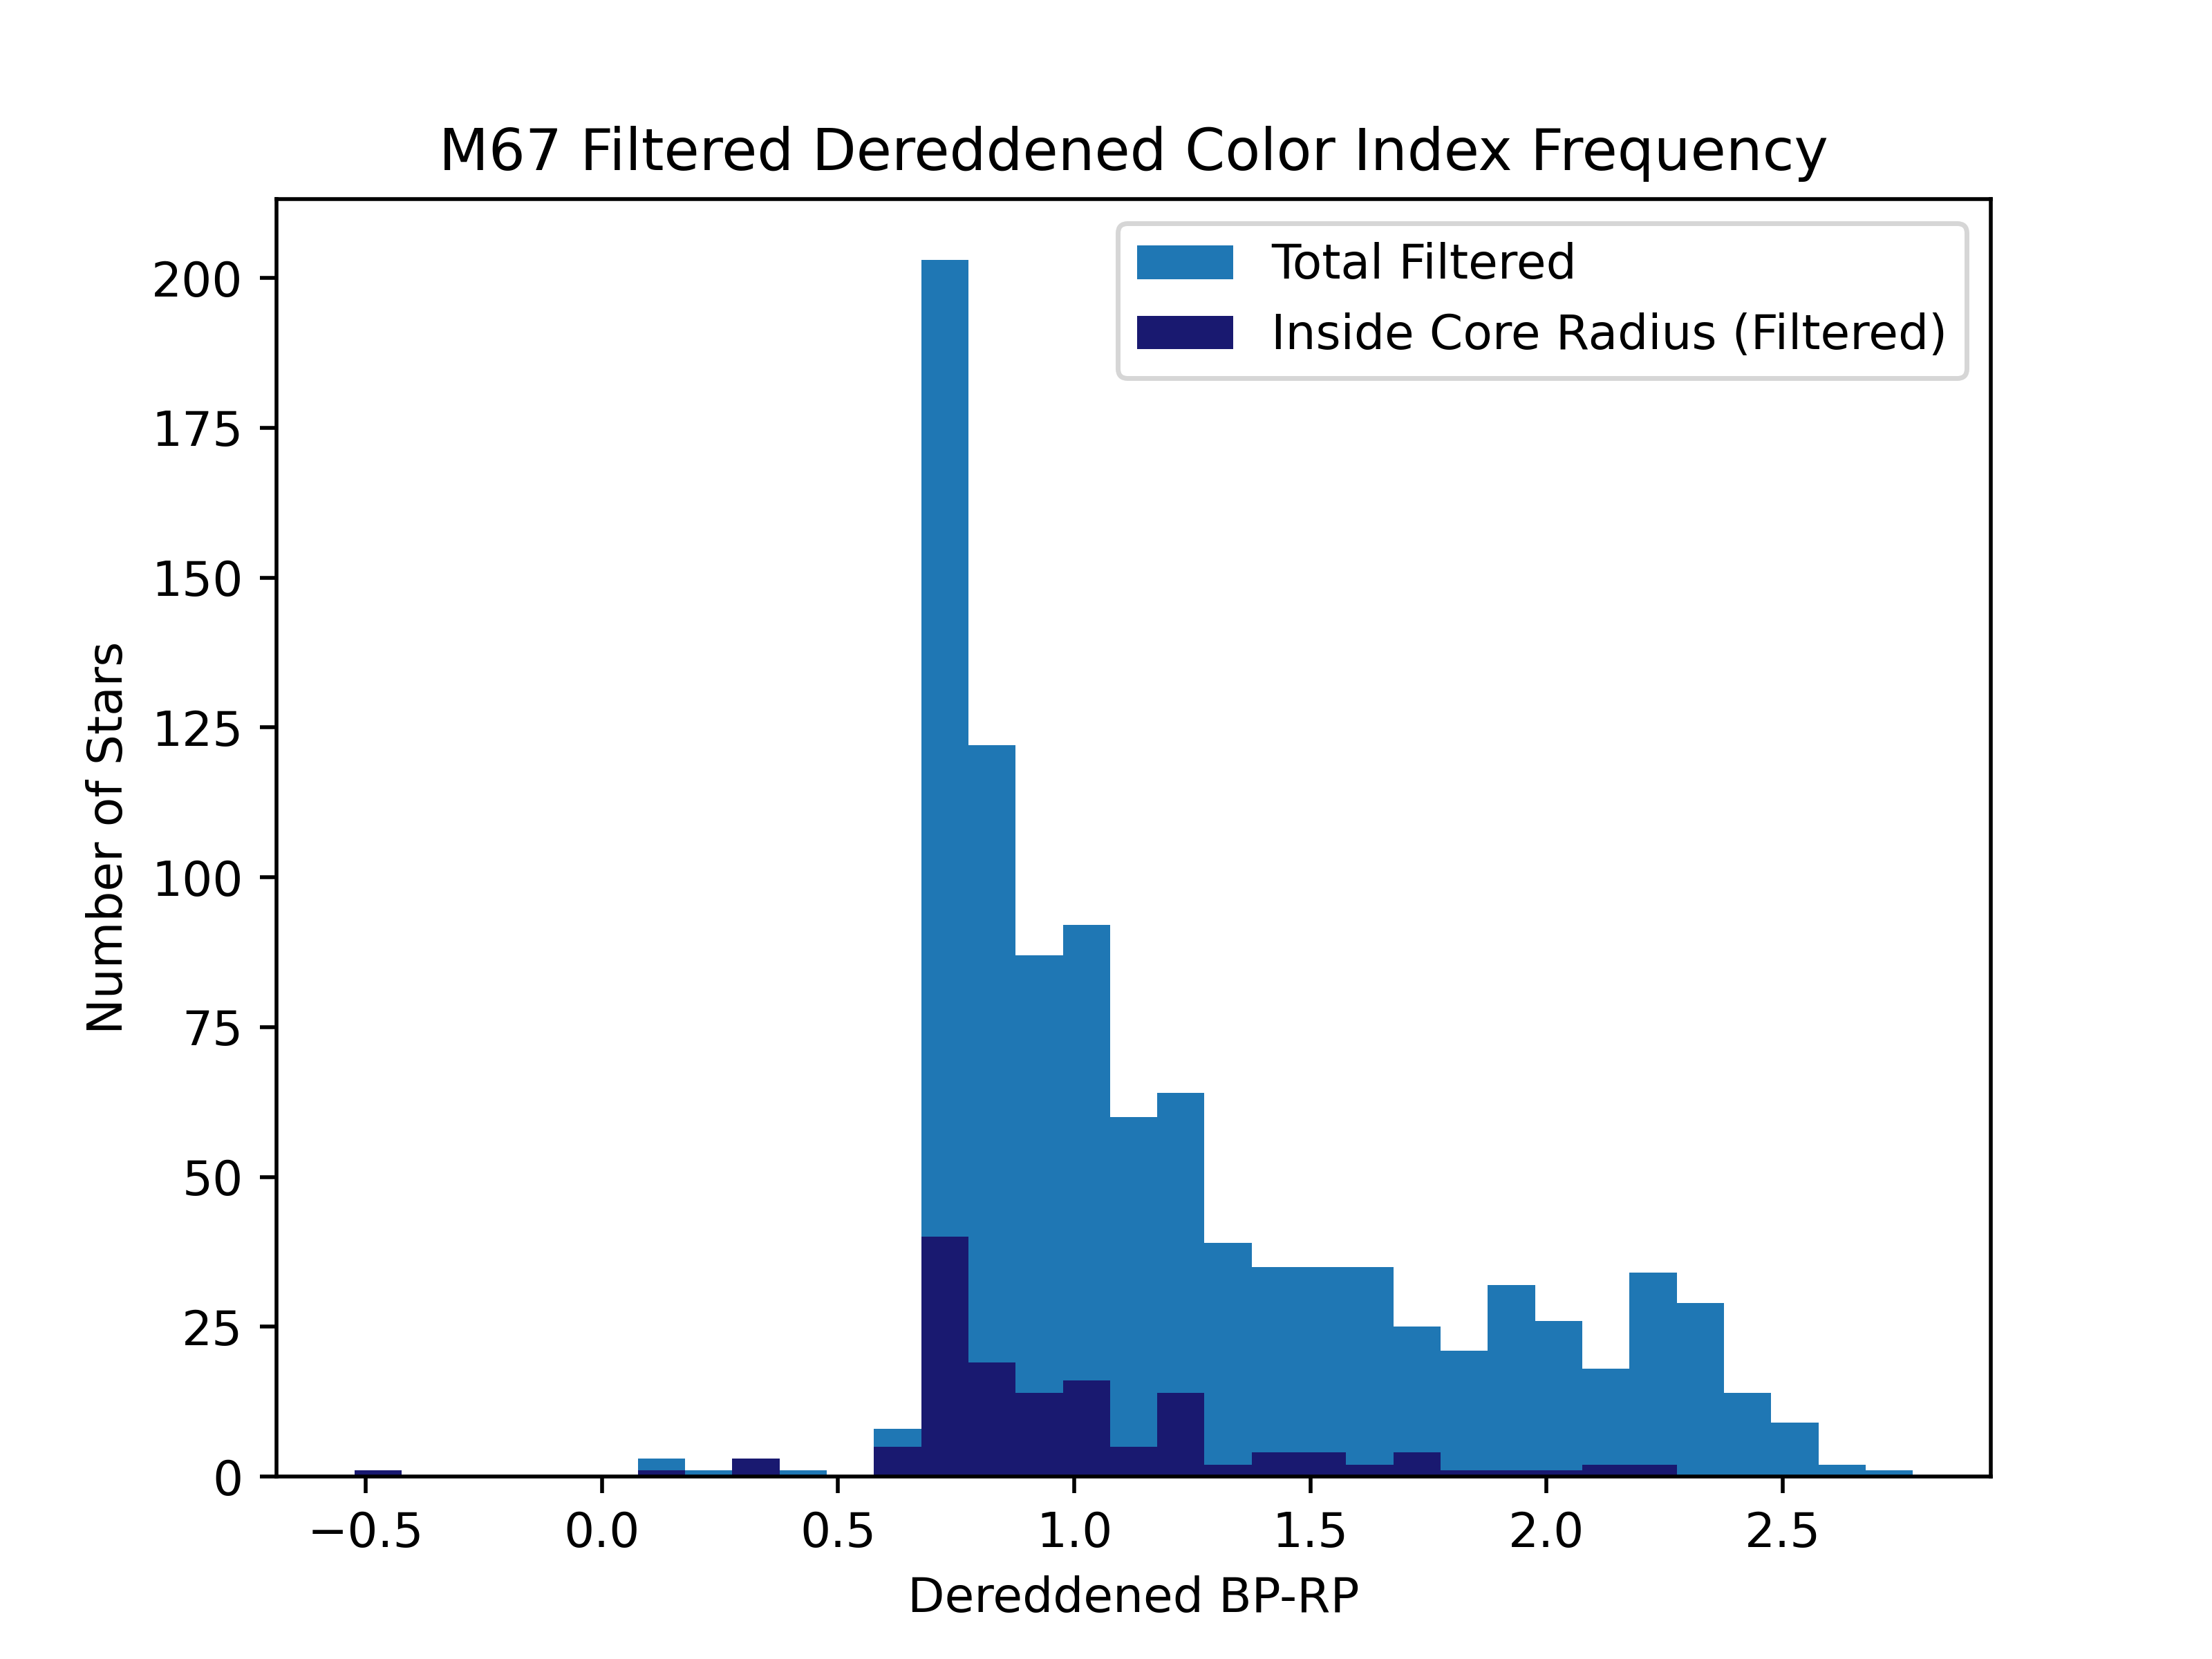
\includegraphics[width=4.75in]{figures/M67_colorFrequency_filtered.png}
    \caption{Histogram of the de-reddened color index of cluster members belonging to Messier 67. Dark blue tracks the stars interior to the cluster core radius, determined by fitting a profile to the number density.}
    \label{fig:M67_color_hist}
\end{figure}

\section{Uncertainties and Potential Biases} \label{sec:error}

One of the main concerns in analyzing trends in the populations of stellar clusters is the presence of existing uncertainties in the data, as well as the steps taken to minimize additional uncertainties introduced in the processing of the data. Gaia tabulates typical uncertainties for its astrometric and photometric properties based on the approximate magnitude. These are summarized in Figure \ref{fig:gaia_table}, taken from the Gaia documentation\protect{\cite{gaia_uncertainties}}. As a rule of thumb, the uncertainty in one of Gaia's measurements increases roughly by a factor of 10 with every increase of 3 to 4 magnitudes. For some measurements, like parallax, this means that at the fainter end of things, below around 19th magnitude, uncertainty in a measurement can become an appreciable fraction of the recorded value. In the clusters we have sampled, the mean ratio of uncertainty in parallax to parallax itself ranges from around 5\% in the nearest clusters, to around 25\% in the furthest, faintest cluster.

\begin{figure}[]
    \centering
      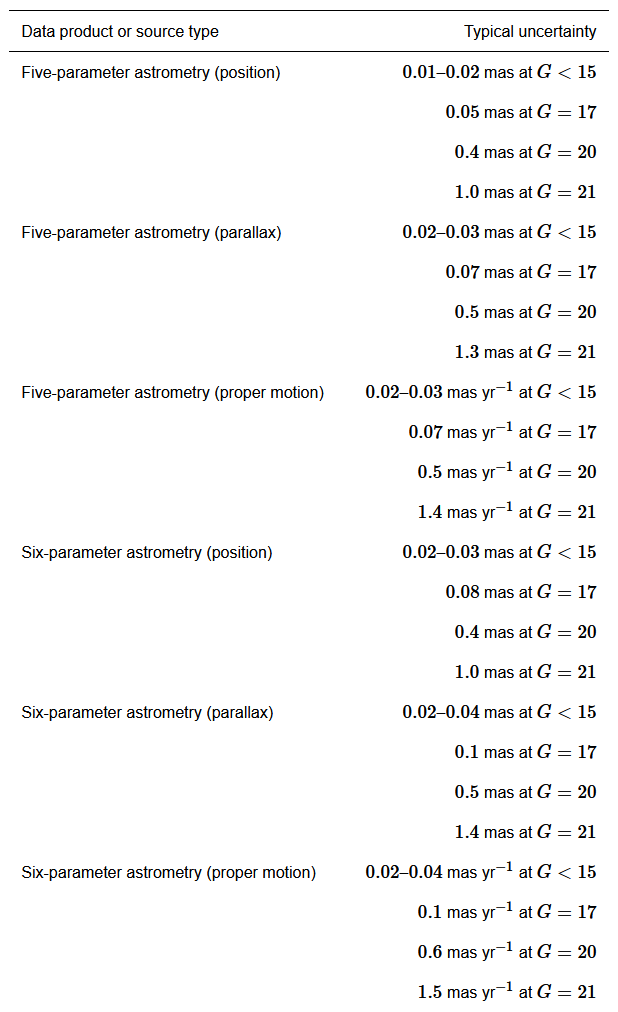
\includegraphics[width=3.5in]{figures/gaia_table1.png}
      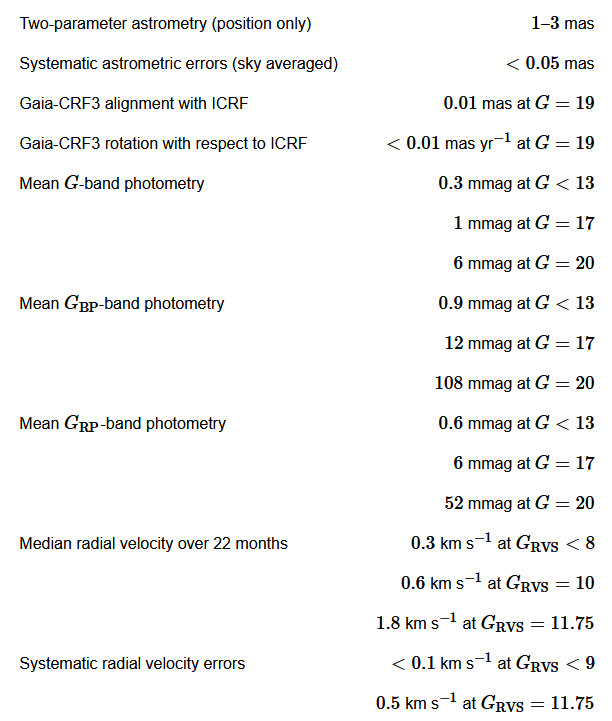
\includegraphics[width=3.5in]{figures/gaia_table2.png}
    \caption{Reproduction of the standard uncertainties summary table from the Gaia documentation\protect{\cite{gaia_uncertainties}}.}
    \label{fig:gaia_table}
\end{figure}

As for accounting for these uncertainties, the handling and propagation depends on the process. For the cluster member identification and filtration process, the fractional uncertainty in the measurements relevant to filtering the cluster is relatively small, and therefore is not included in any calculations. The limits placed on parallax and proper motion tend to be wide enough that uncertainties in those measurements will not disqualify a significant number of ``real" cluster members, nor will it qualify a significant number of contaminant stars. Where it matters most is perhaps in the case of parallax, where the fractional uncertainty is often over 10\%. In these cases, however, the assumed accuracy of the $3\sigma$ cut on mean parallax is unaffected, as the standard deviation is correspondingly larger. In the isochrone fitting process, there is little purpose in tracking and accounting for the uncertainties in magnitudes and color indices. This is in part because the fractional uncertainties for those measurements are sufficiently small, and in part because of the coarse step size between many of the synthetic isochrones.


\subsection{Brightness Bias} \label{sec:bias}

With one of the main properties of interest to us being the masses of stars and clusters, we gradually became concerned with the potential existence of biases that can arise from the physical limits of the instruments on board Gaia. Gaia is only able to observe objects as faint as an apparent magnitude of 21, meaning that the low mass, faint stars in more distant and obscured clusters can be lost to this cutoff. Additionally, several clusters had small portions of their lower main sequence further cut by the filtering process due to a rapid spike in multivariate uncertainty, as detailed in Section \ref{sec:filtering}. In order to ensure that the comparisons of average mass and mass profile fitting is unbiased by these cutoffs, we needed to enforce our own cutoff that ensured the lowest mass stars were not being included in any estimations of average mass or mass drop off.

In theory, the main sequence tracks of all of the open cluster populations should roughly line up on a CMD, if all other variables were accounted for. To make this kind of comparison both faster computationally and easier to visualize, we've assembled a scatter plot using only the proxy points that represent a cluster's true CMD. In Figure \ref{fig:pop_cmd_apparent}, we can see that the uncorrected apparent magnitude observations do not line up neatly, though this is to be expected given the axes are as observed. Using parallax to get a distance estimate for the cluster, however, allows us to correct these apparent magnitude observations to absolute magnitude, as discussed in Section \ref{sec:iso}. The other factor to account for, as we had to worry about when fitting isochrones, is the joint process of interstellar reddening and extinction. Thankfully for the purpose of this process, we already have a best estimate of these two phenomenon from the isochrone fitting routine. 

As a result, we can convert the apparent magnitudes for all of the clusters to their absolute magnitudes, and correct for the effects of interstellar reddening and extinction. The results of these corrections can be seen in Figure \ref{fig:pop_cmd_absolute}. This figure in and of itself is reassuring in several ways. Firstly, it's nice to reaffirm theory with observational data, especially when a new set of data like Gaia becomes available. Secondly, the strong overlap in the main sequences of all of the sampled clusters suggests that our methodology and results for finding the interstellar reddening and extinction are relatively robust. We can also use this diagram to find a location to put our artificial limit on the main sequence. In Figure \ref{fig:pop_cmd_shifted}, we have artificially spaced out the CMD of each cluster to better visualize the effects of a cutoff. The selected cutoff of a de-reddened color index of $BP-RP = 1.6$, keeping stars bluer than this limit and discarding the redder, lower mass stars with a greater color index. This gives us a good balance of preserving much of the main sequence and post-turnoff while also ensuring that no low-light bias is present in our results. The limit enforcement is only applied below the cluster's turning point, to ensure that post-turnoff features are not also cut from the data. 

\begin{figure}[]
    \centering
      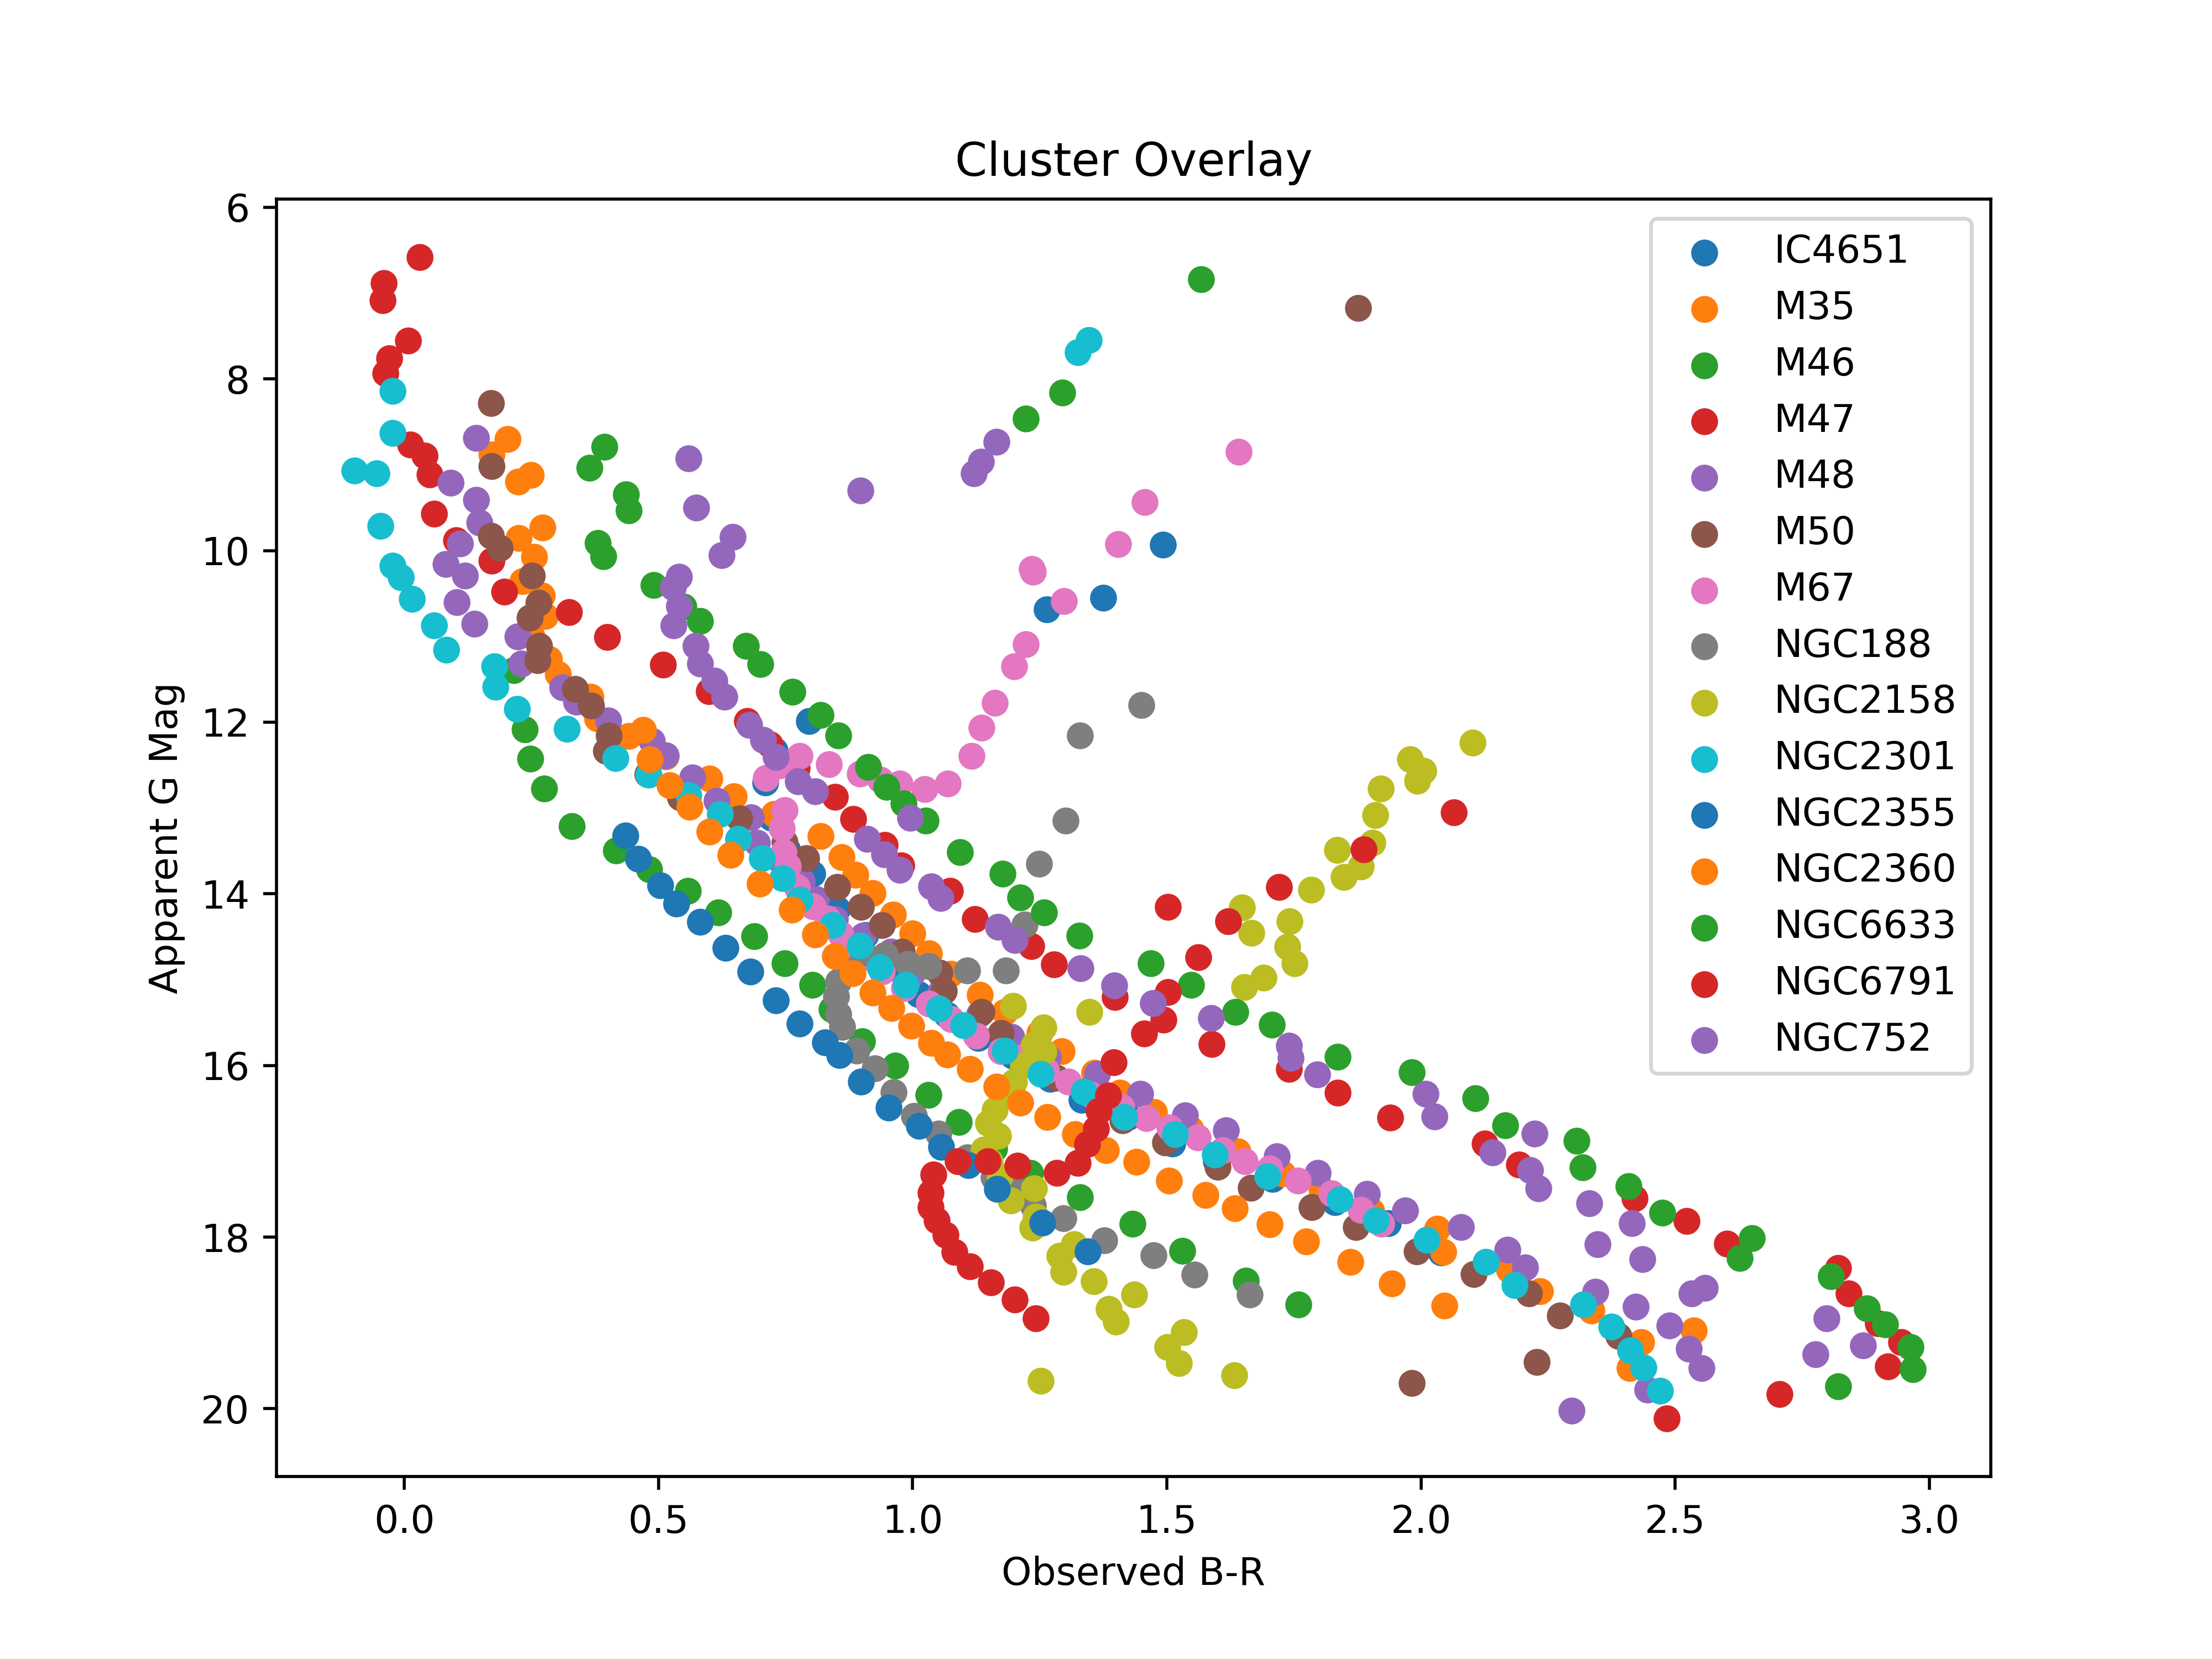
\includegraphics[width=4.75in]{figures/pop_cmd_apparent.png}
    \caption{Overlay of the proxy points used for the fitting of 15 open clusters. Both axes are in apparent magnitudes, and have not been corrected for distance or ISM based extinction or reddening. The span of magnitudes is quite large, with main sequence turnoff points appearing from nearly 6th magnitude all the way to around 17th magnitude.}
    \label{fig:pop_cmd_apparent}
\end{figure}

\begin{figure}[]
    \centering
      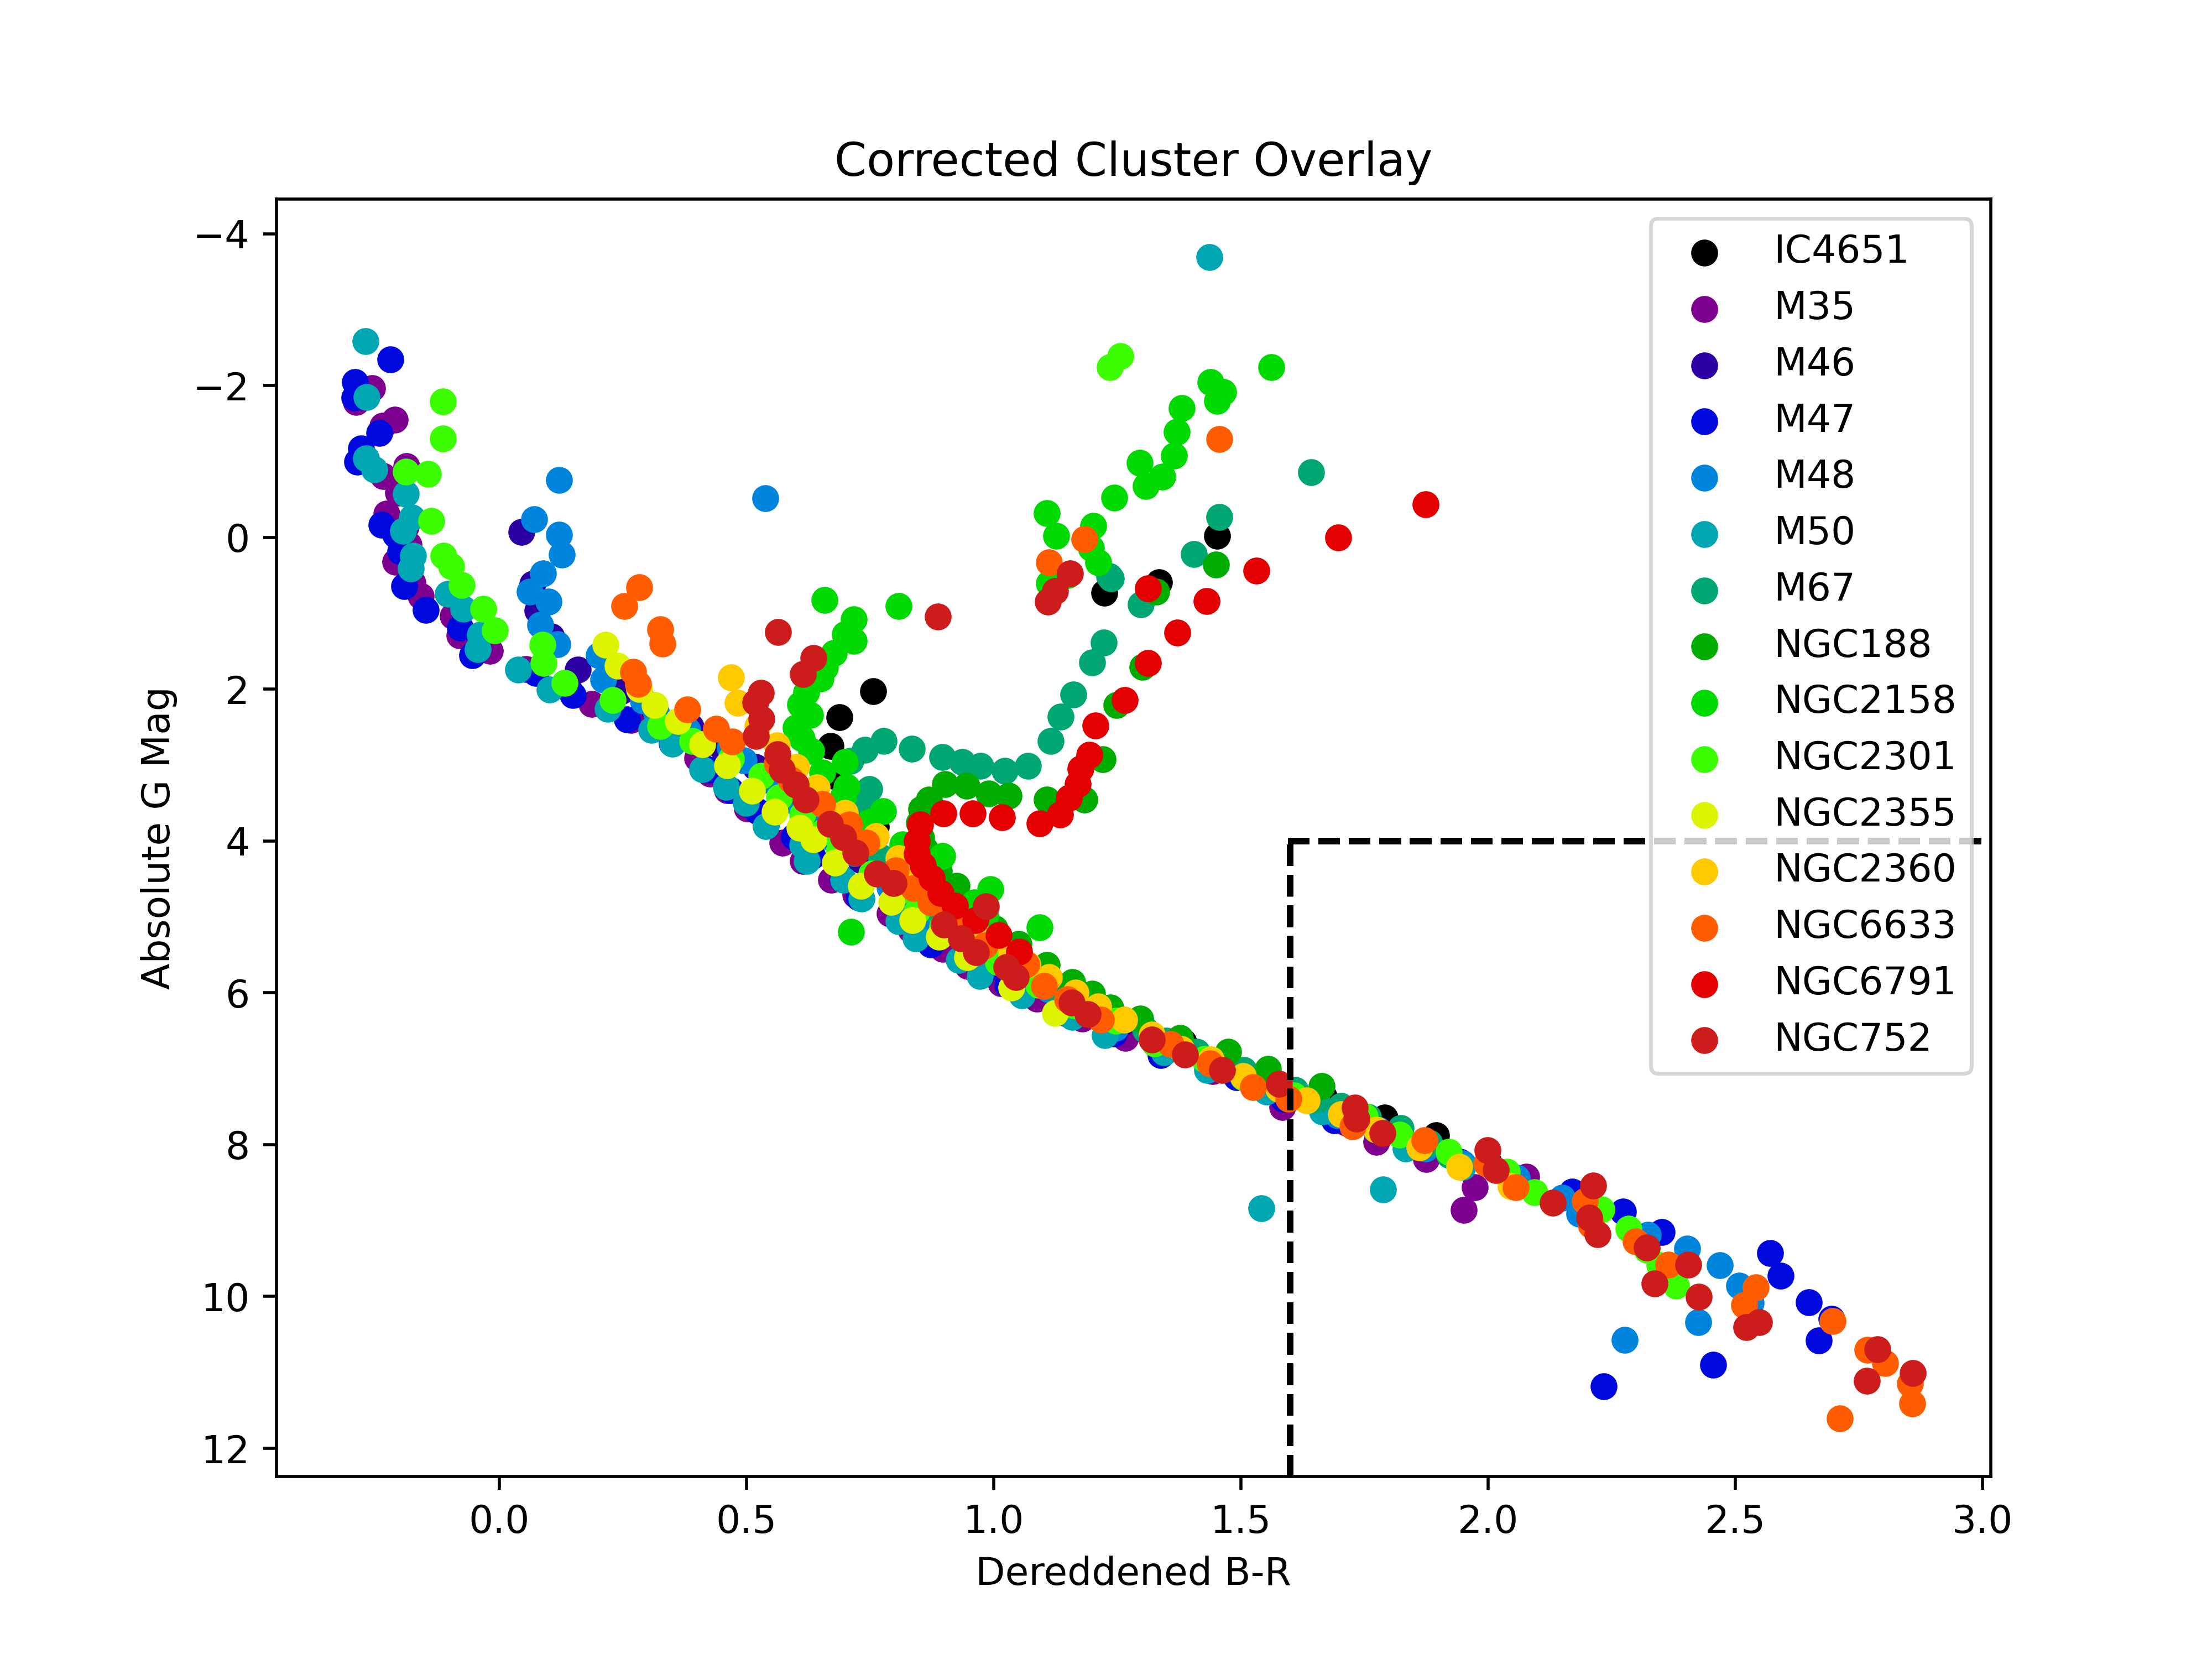
\includegraphics[width=4.75in]{figures/pop_cmd_absolute.png}
    \caption{A plot created from the values in Figure \ref{fig:pop_cmd_apparent}, that have been adjusted by the distance modulus for the cluster and corrected for interstellar reddening and extinction. The net effect of this is that the main sequences of the clusters line up quite nicely, with the only notable departures being where the turnoff point is located. Not only does this plot serve to validate theory with empirical observations, but it also serves as a check on the methods for determining interstellar reddening and extinction, which are necessary in the alignment of the CMDs. The box on the lower right outlines the region of the CMD that is excluded for the purposes of removing detector limit selection bias. See Section \ref{sec:bias} for more details.}
    \label{fig:pop_cmd_absolute}
\end{figure}

\begin{figure}[]
    \centering
      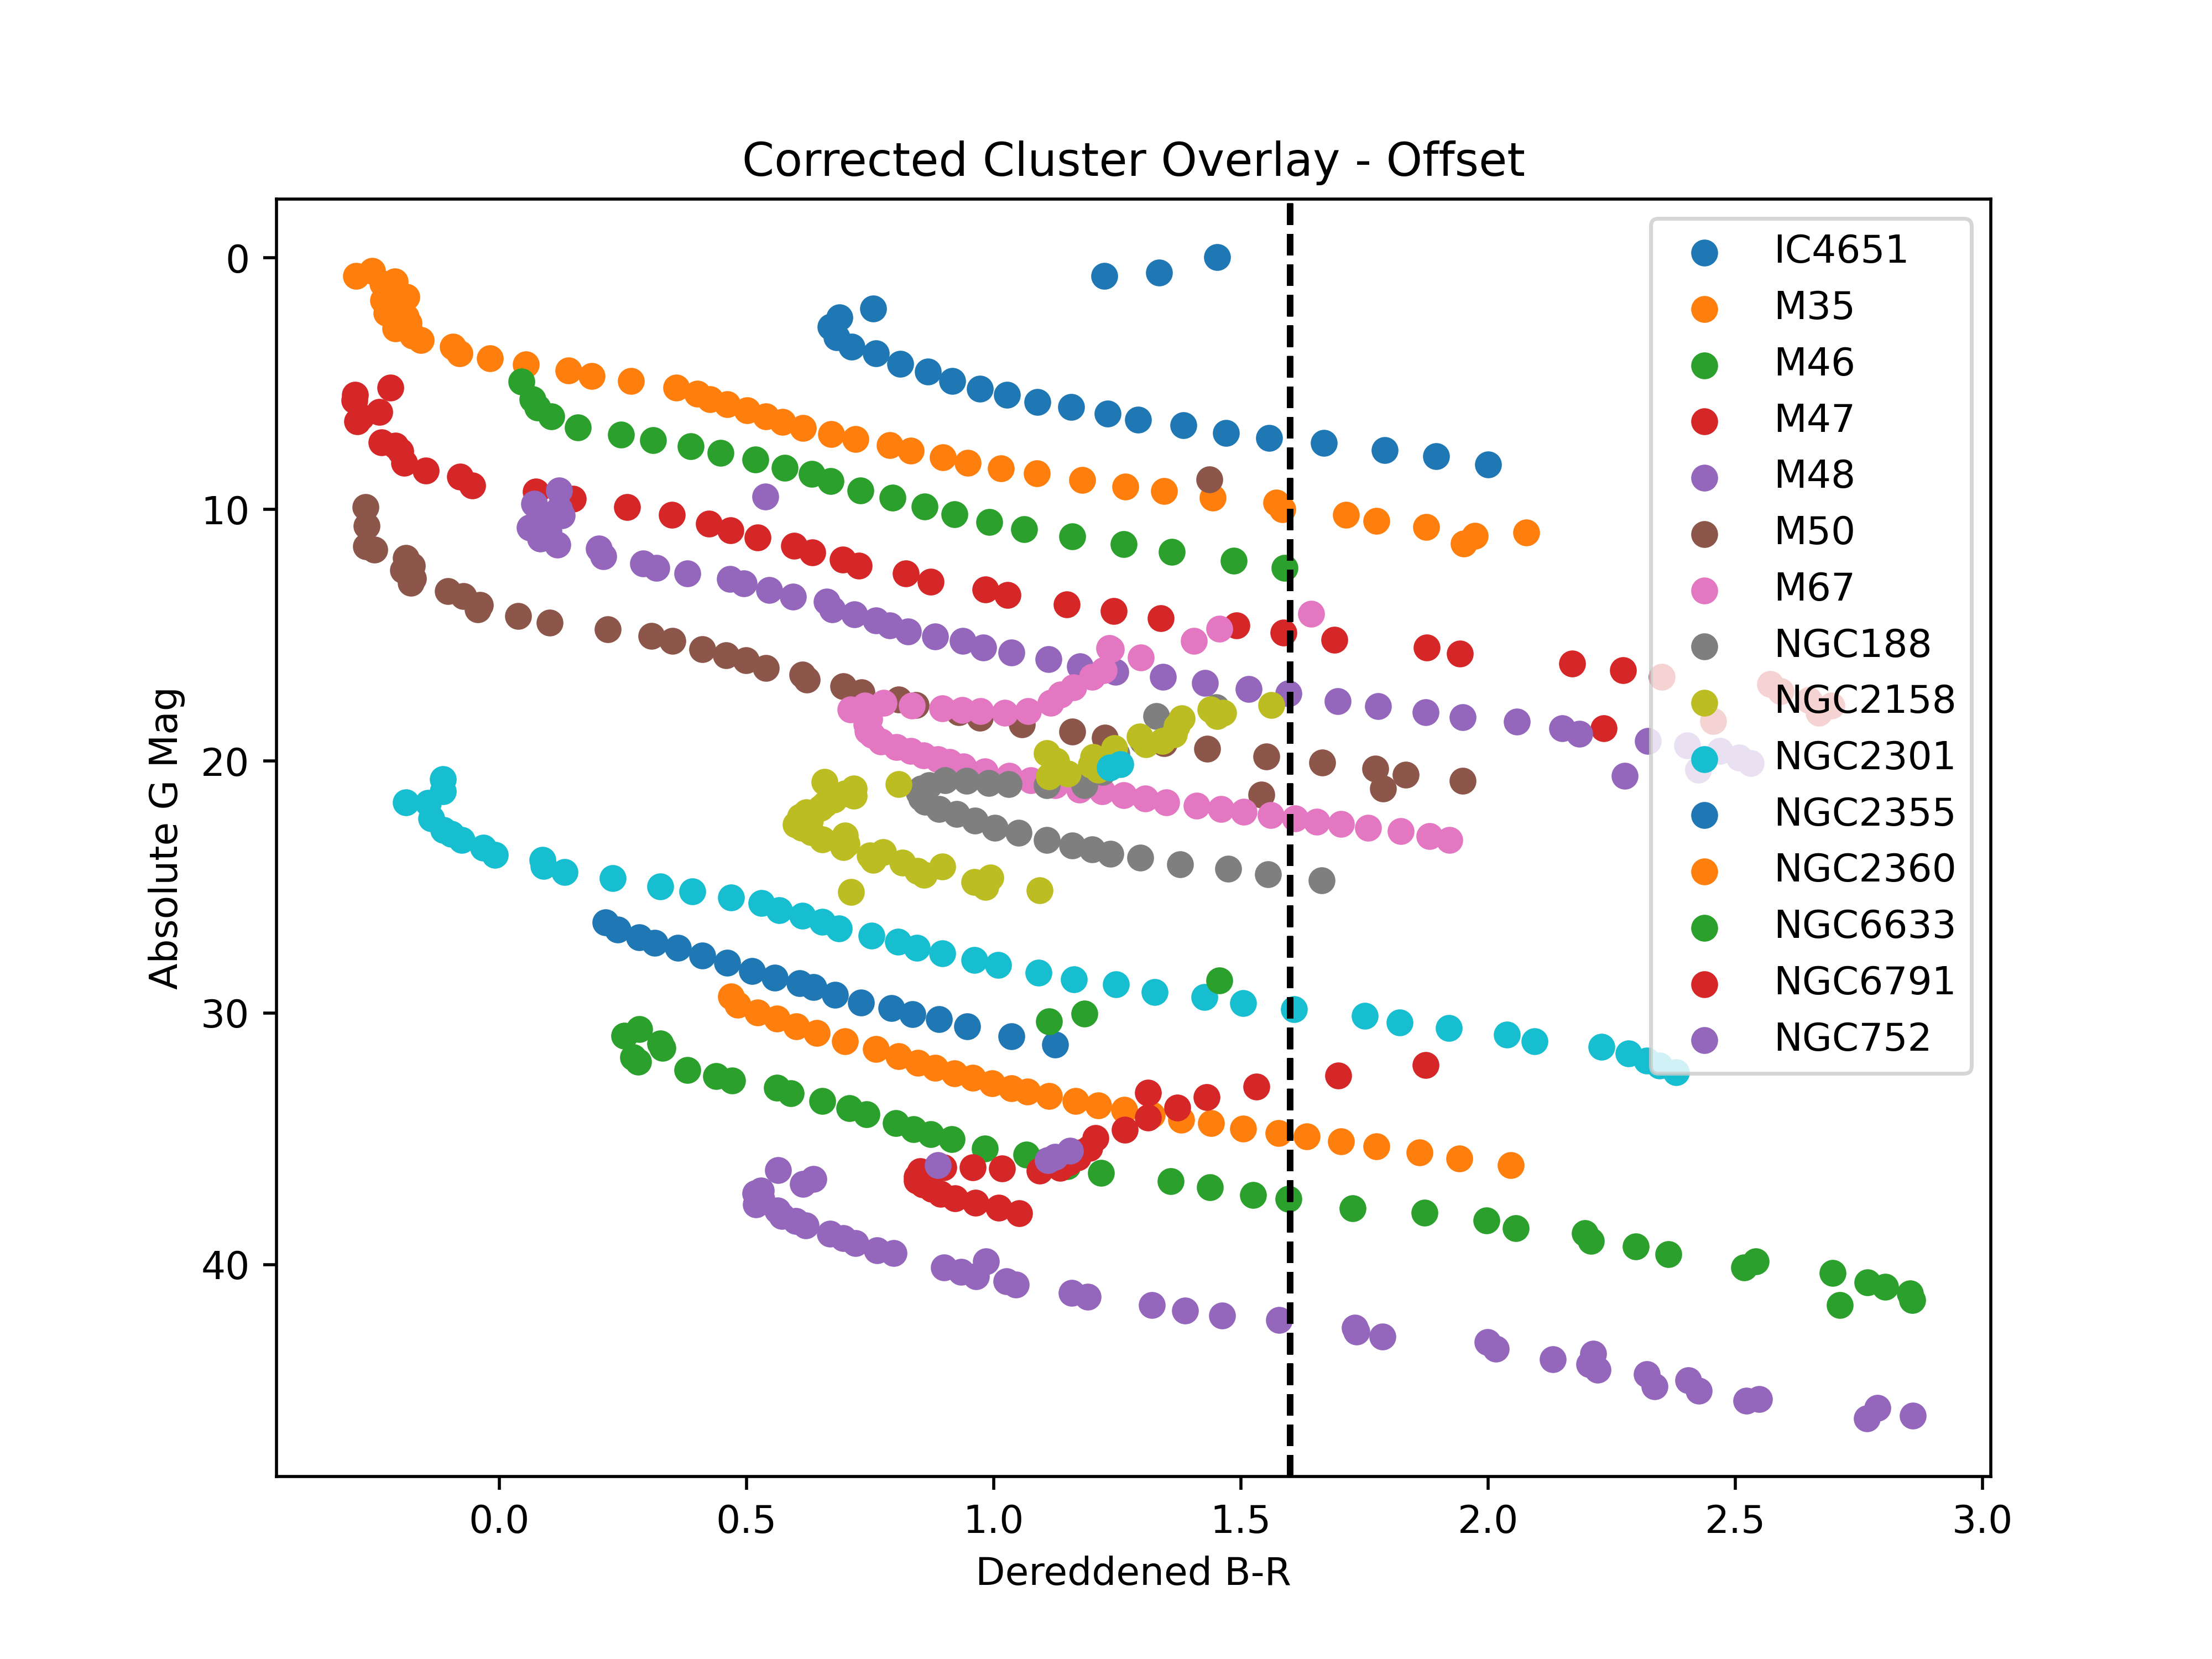
\includegraphics[width=4.75in]{figures/pop_cmd_shifted.png}
    \caption{Duplicate of Figure \ref{fig:pop_cmd_absolute} with the cluster CMDs spaced vertically by an arbitrary amount. This is done to visualize the relative effect of the $BP-RP = 1.6$ cutoff on each cluster.}
    \label{fig:pop_cmd_shifted}
\end{figure}

Using this truncated data set, we've again followed several of the aforementioned procedures. Figure \ref{fig:M67_num_density_bounded} shows the number density of the cluster members in the upper-bounded data set. Similarly, Figure \ref{fig:M67_average_mass_bounded} shows the average mass as a function of distance for the upper-bounded members. Other diagnostic plots, and the plots for every other cluster sampled, can be found in the relevant sections of the Appendix.

\begin{figure}[]
    \centering
      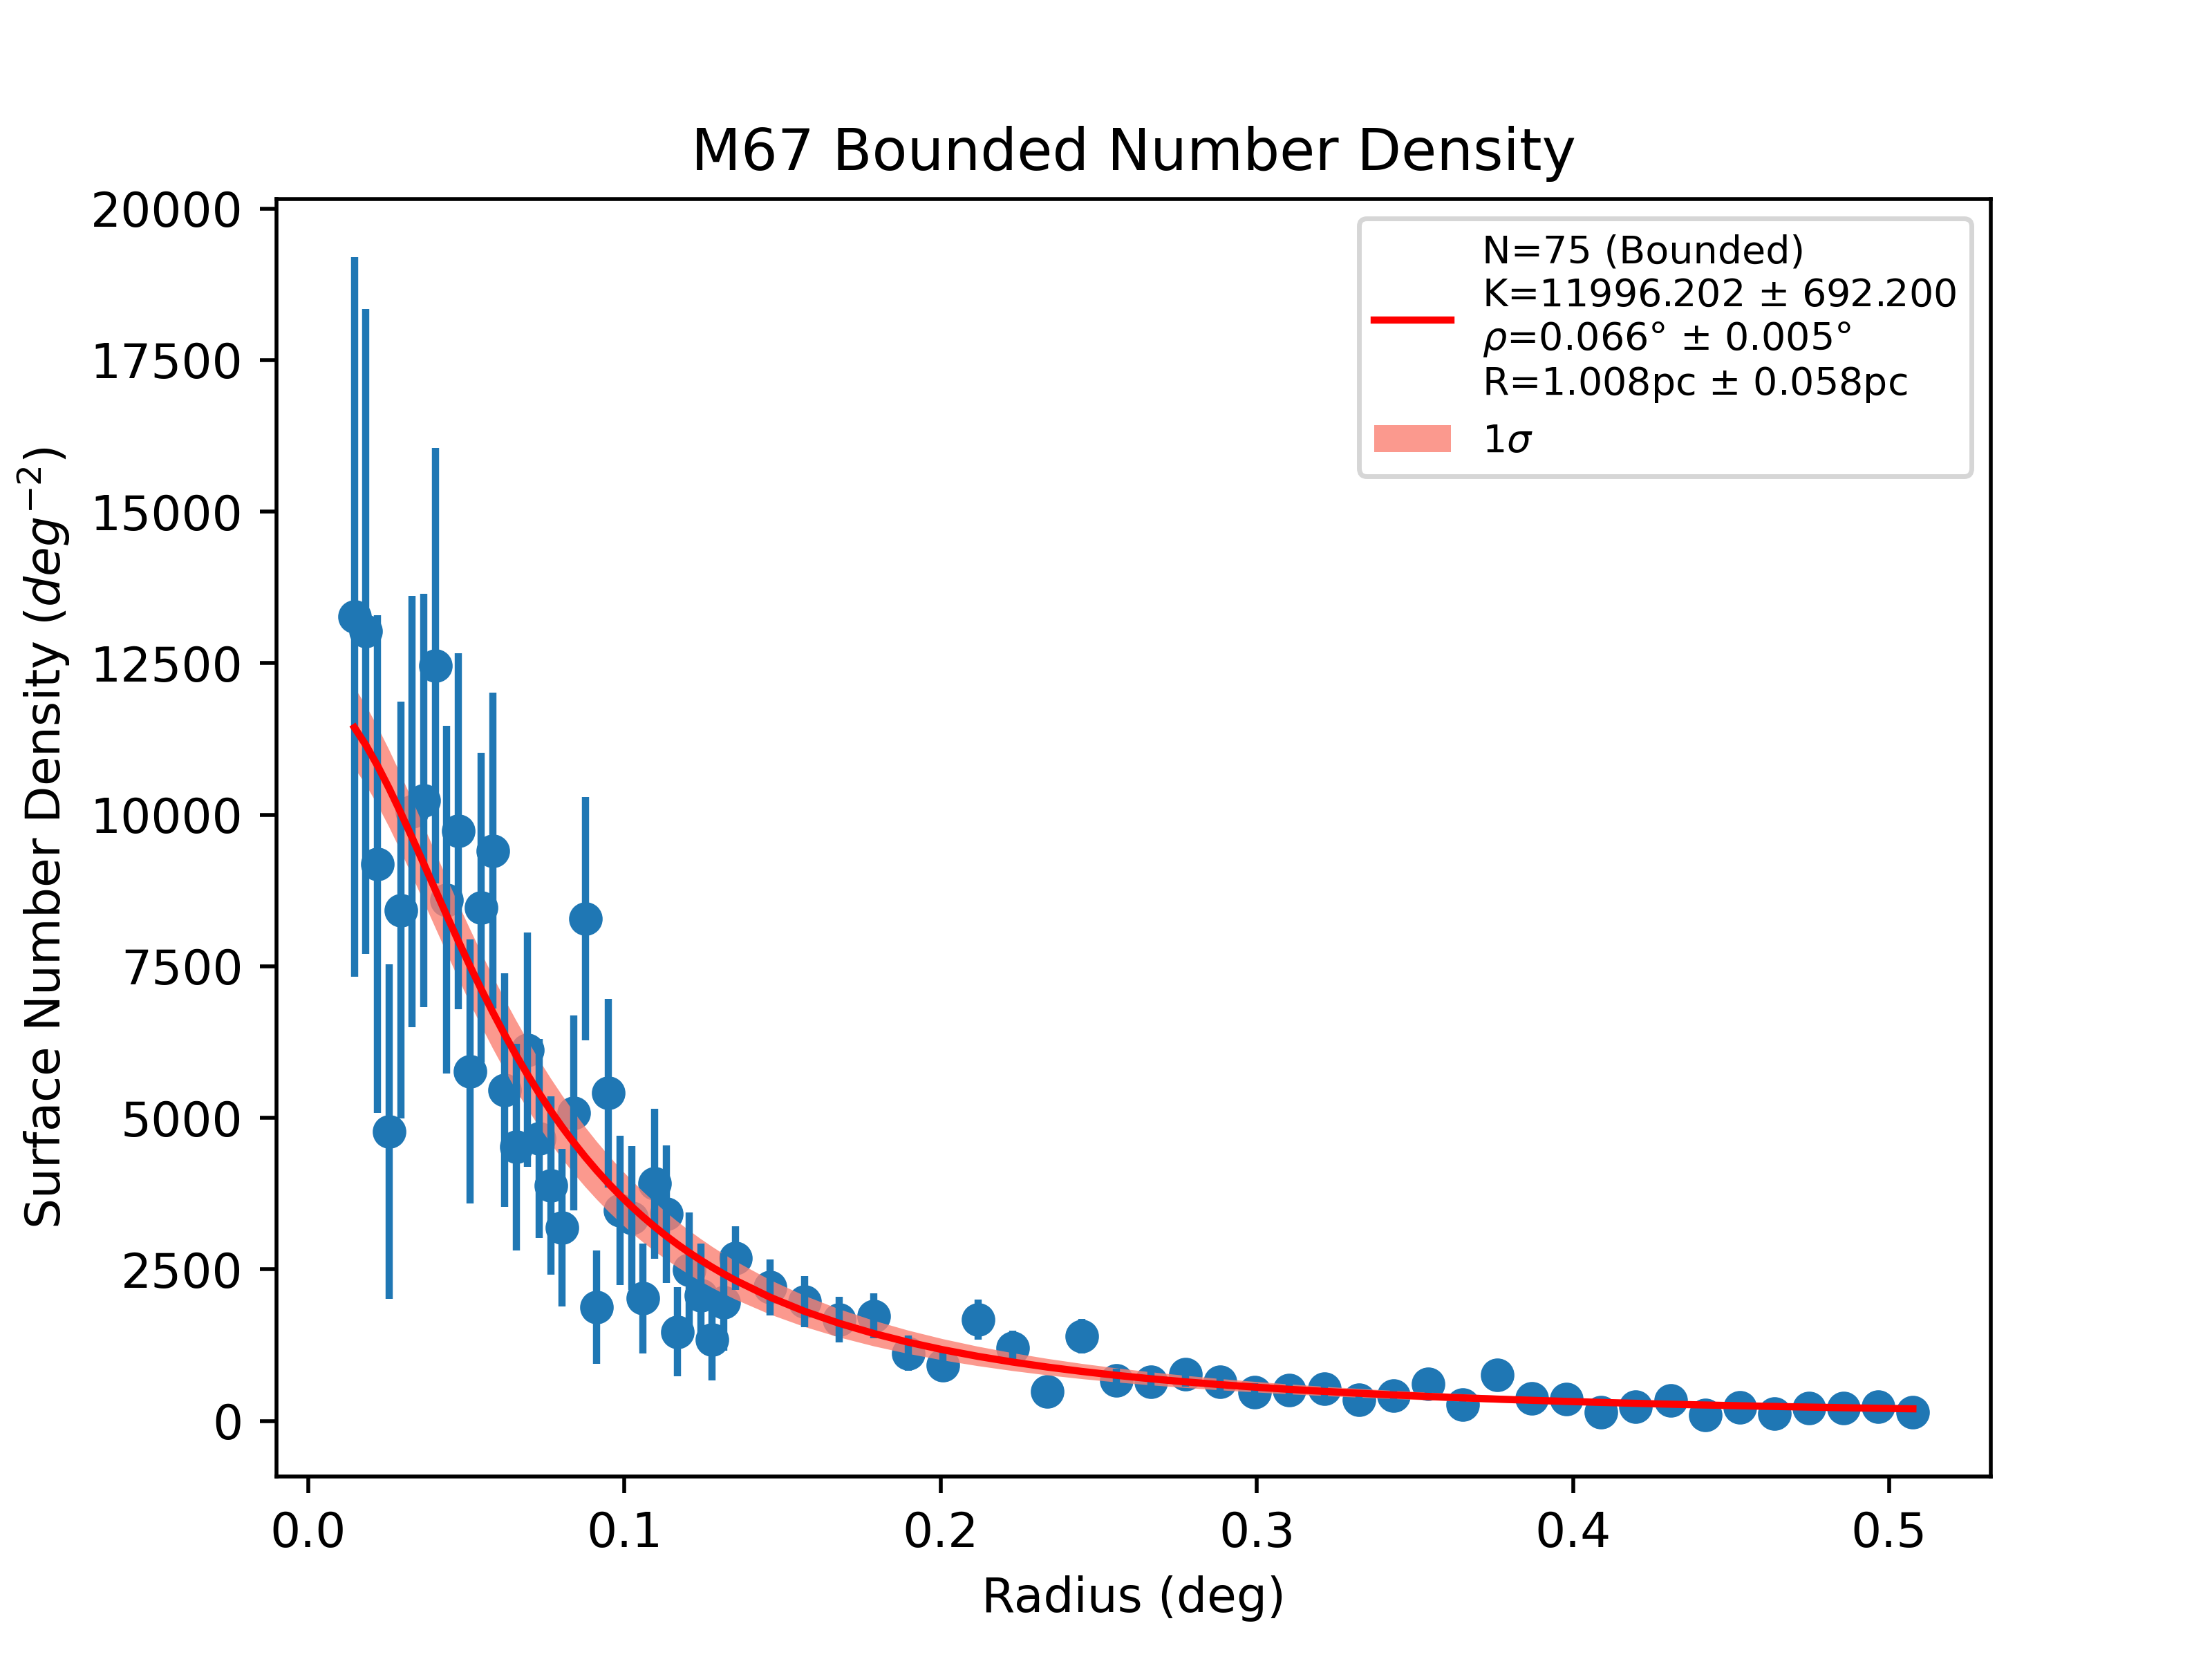
\includegraphics[width=4.75in]{figures/M67_numDensity_bounded.png}
    \caption{Surface number density plot for Messier 67 that was created using only cluster members whose de-reddened BP-RP is less than 1.6, otherwise referred to as the `bounded' members. A smaller number of bins was assigned in order to avoid oversampling, as a significant fraction of M67's cluster members were removed by the BP-RP limit.}
    \label{fig:M67_num_density_bounded}
\end{figure}

\begin{figure}[]
    \centering
      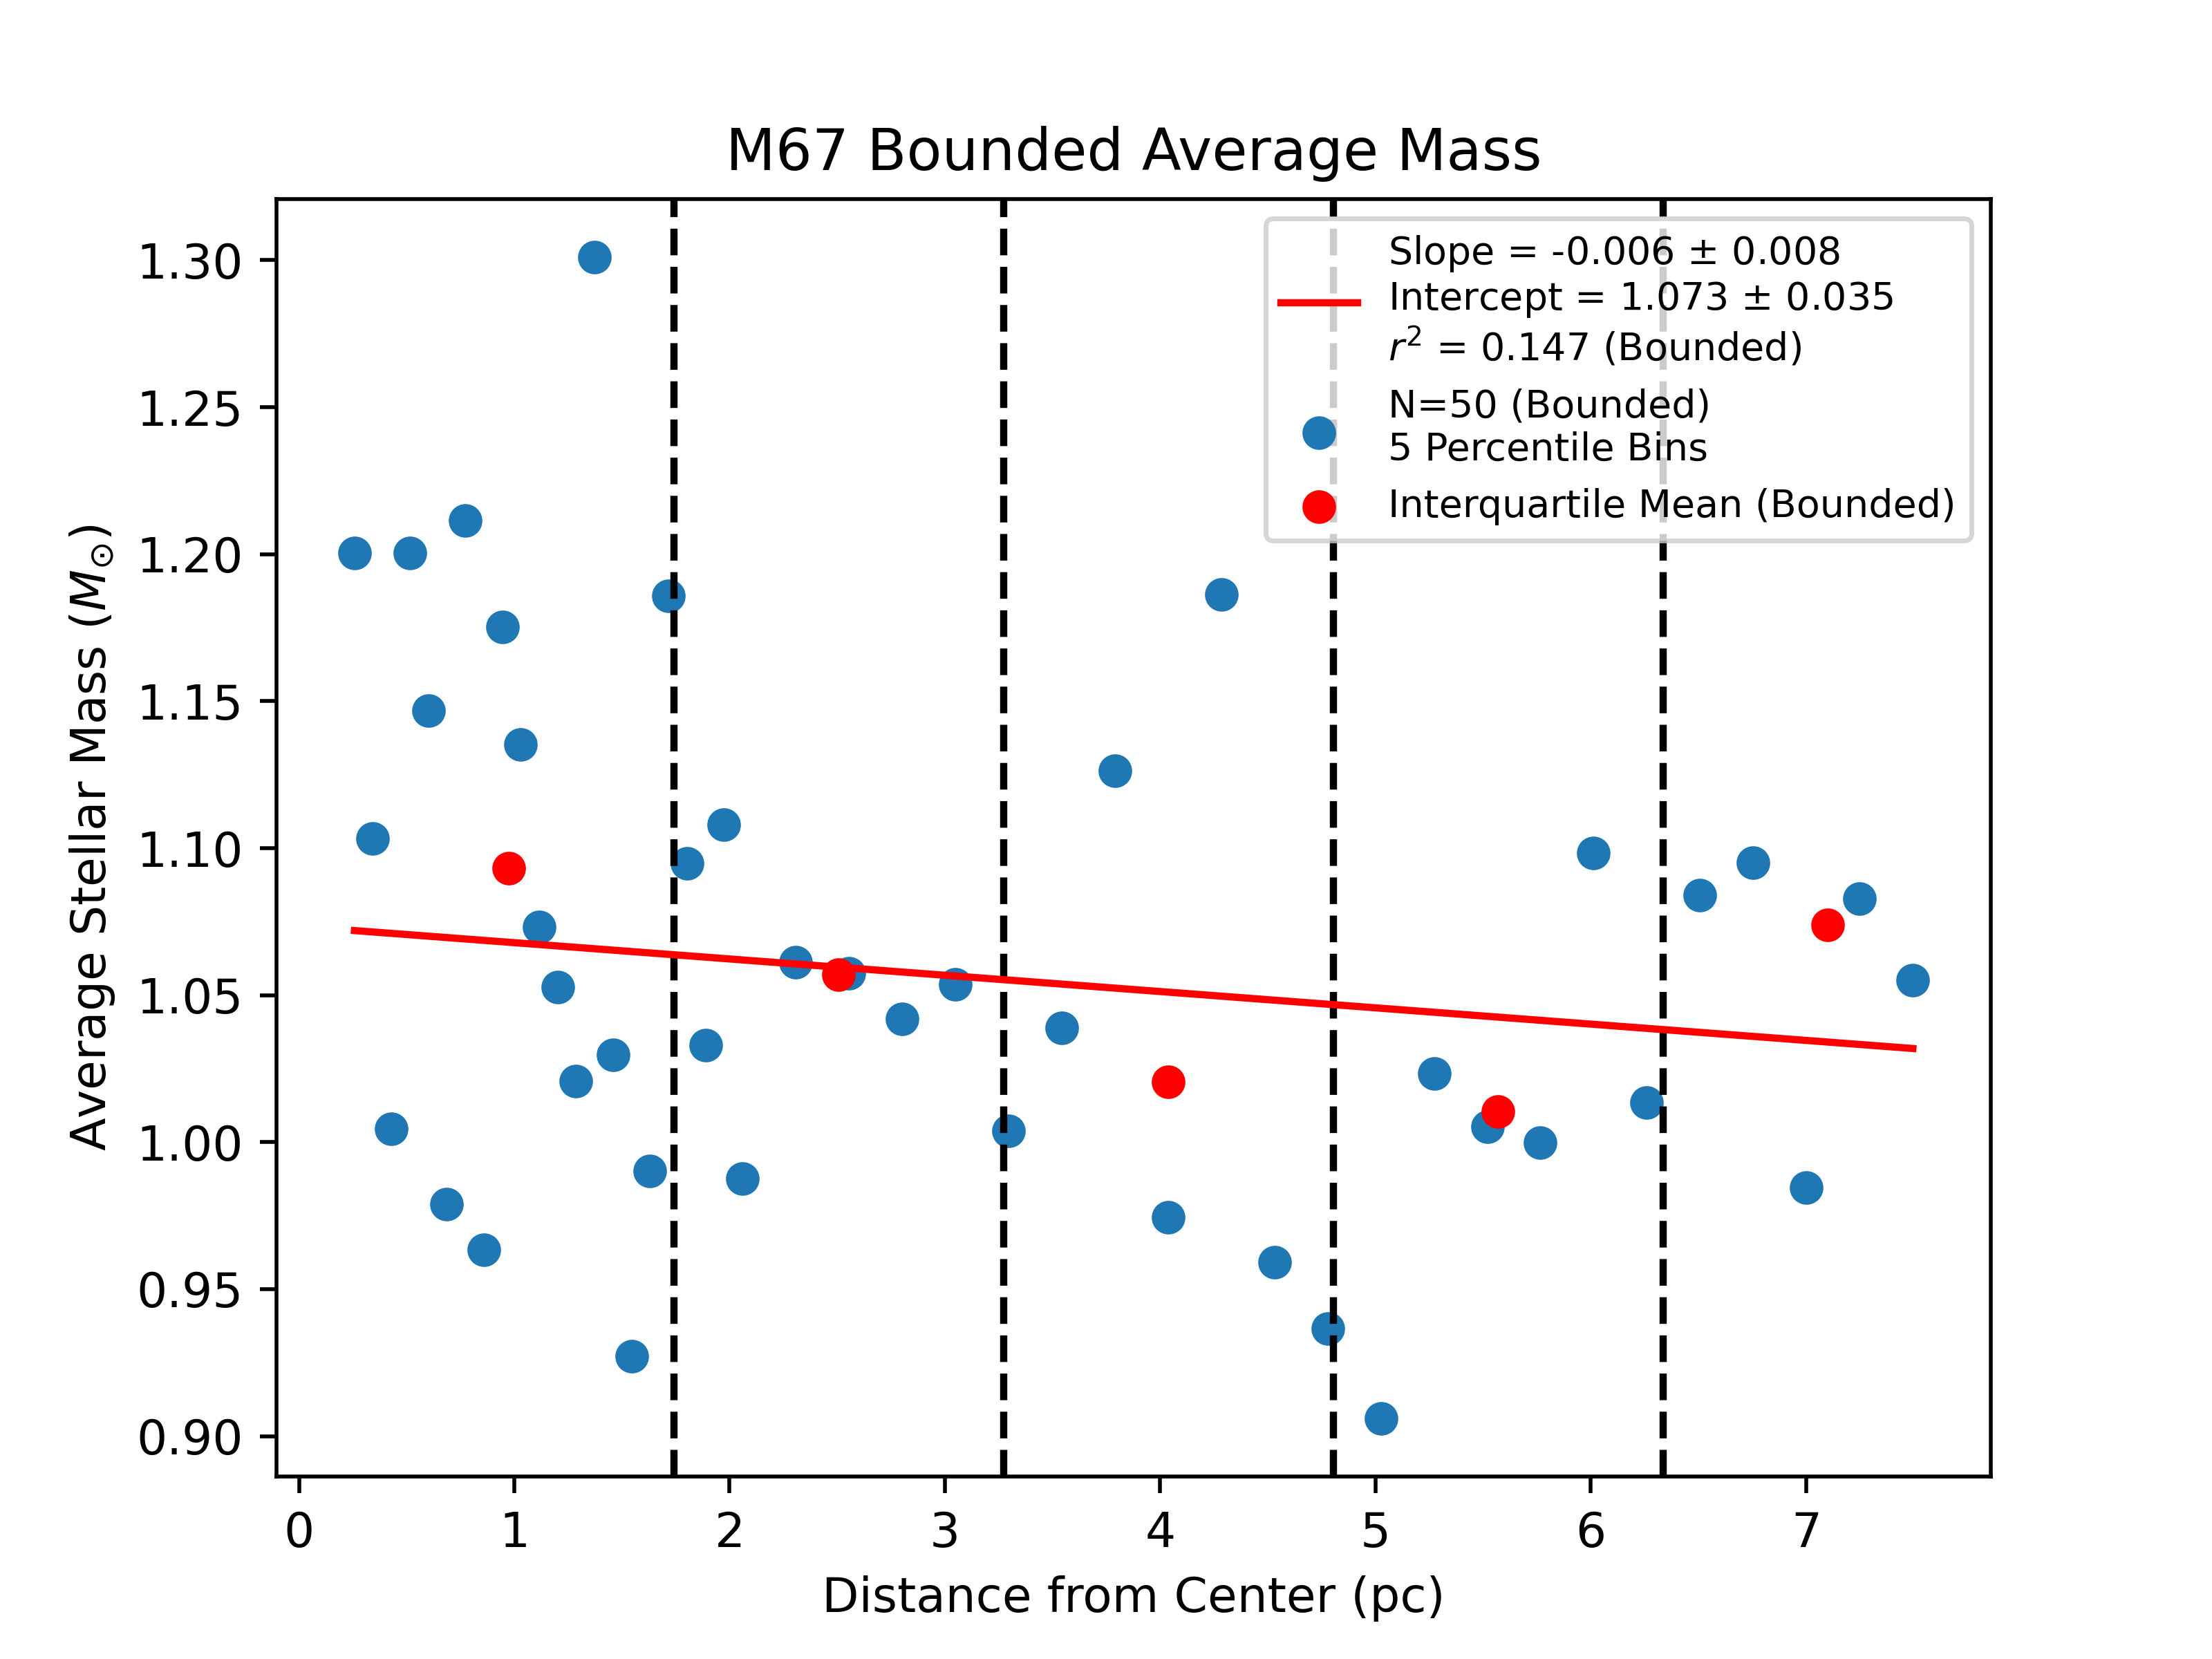
\includegraphics[width=4.75in]{figures/M67_averageMass_bounded.png}
    \caption{Average stellar mass of cluster members in Messier 67, as a function of distance. All values were determined in an equivalent way to Figure \ref{fig:M67_average_mass}, though only the `bounded' cluster members, ones that were not removed by the BP-RP filter, were included. The linear fit to the interquartile mean, shown in red, is of dubious value, as the $r^2$ is considerably small.}
    \label{fig:M67_average_mass_bounded}
\end{figure}


\subsection{Introduced Uncertainties} \label{sec:uncertainty}

Other potential sources of uncertainty arise from the fitting process. The isochrones, or synthetic CMDs, used in the fitting routine have their own limitations. The age range of the MIST\protect{\cite{mist}} isochrones varies quite a bit, but for clusters on the order of 4-6 Gyr, the variance in ages is relatively coarse. Even coarser are the variances in metallicity. $[\frac{Fe}{H}]$ is varied only in increments of 0.25 and 0.5, though the total coverage of values has been sufficient to fit our sample of open clusters. $[\frac{\alpha}{Fe}]$, however, does not have any variance in the current revision of MIST\protect{\cite{mist}} isochrones. Earlier versions of our work, which utilized a different set of isochrones, found that some clusters did have an improvement in overall isochrone fit from variances in $[\frac{\alpha}{Fe}]$. As such, we can only assume some degree of uncertainty arises from the omission of variations in $[\frac{\alpha}{Fe}]$. As for the best reported values for age, metallicity, and reddening, we assign an estimated uncertainty as large as the interval between the best-fit values and their nearest neighbors. In other words, our confidence in a particular increment of age and metallicity made available to us is near absolute, but beyond that we are unable to further constrain the uncertainty.

Another dubious degree of uncertainty in values determined through isochrone fitting arises from the lower main sequence. The isochrone fitting process tends to produce excellent fits to the majority of the main sequence, turnoff, and even post-turnoff regions of the CMD. However, the best fitting isochrones in the case of some clusters tend to diverge from the observational data on the tail end of the main sequence. This is usually seen as the isochrone projecting fainter than the observed cluster members are observed to be, at a given color. This can be best seen in the case of Messier 67, shown in Figure \ref{fig:M67_iso}. In other clusters, the majority of the main sequence, lower end included, is fit perfectly well by eye, but part or most of the turnoff shape is not present in the observed CMD. As such, the accuracy of a fit is limited to how well the main sequence and any post-turnoff features are fit. An example of this phenomena, where the turnoff region is ``absent", can be seen in Figure \ref{fig:NGC2360_iso}.

\begin{figure}[]
    \centering
      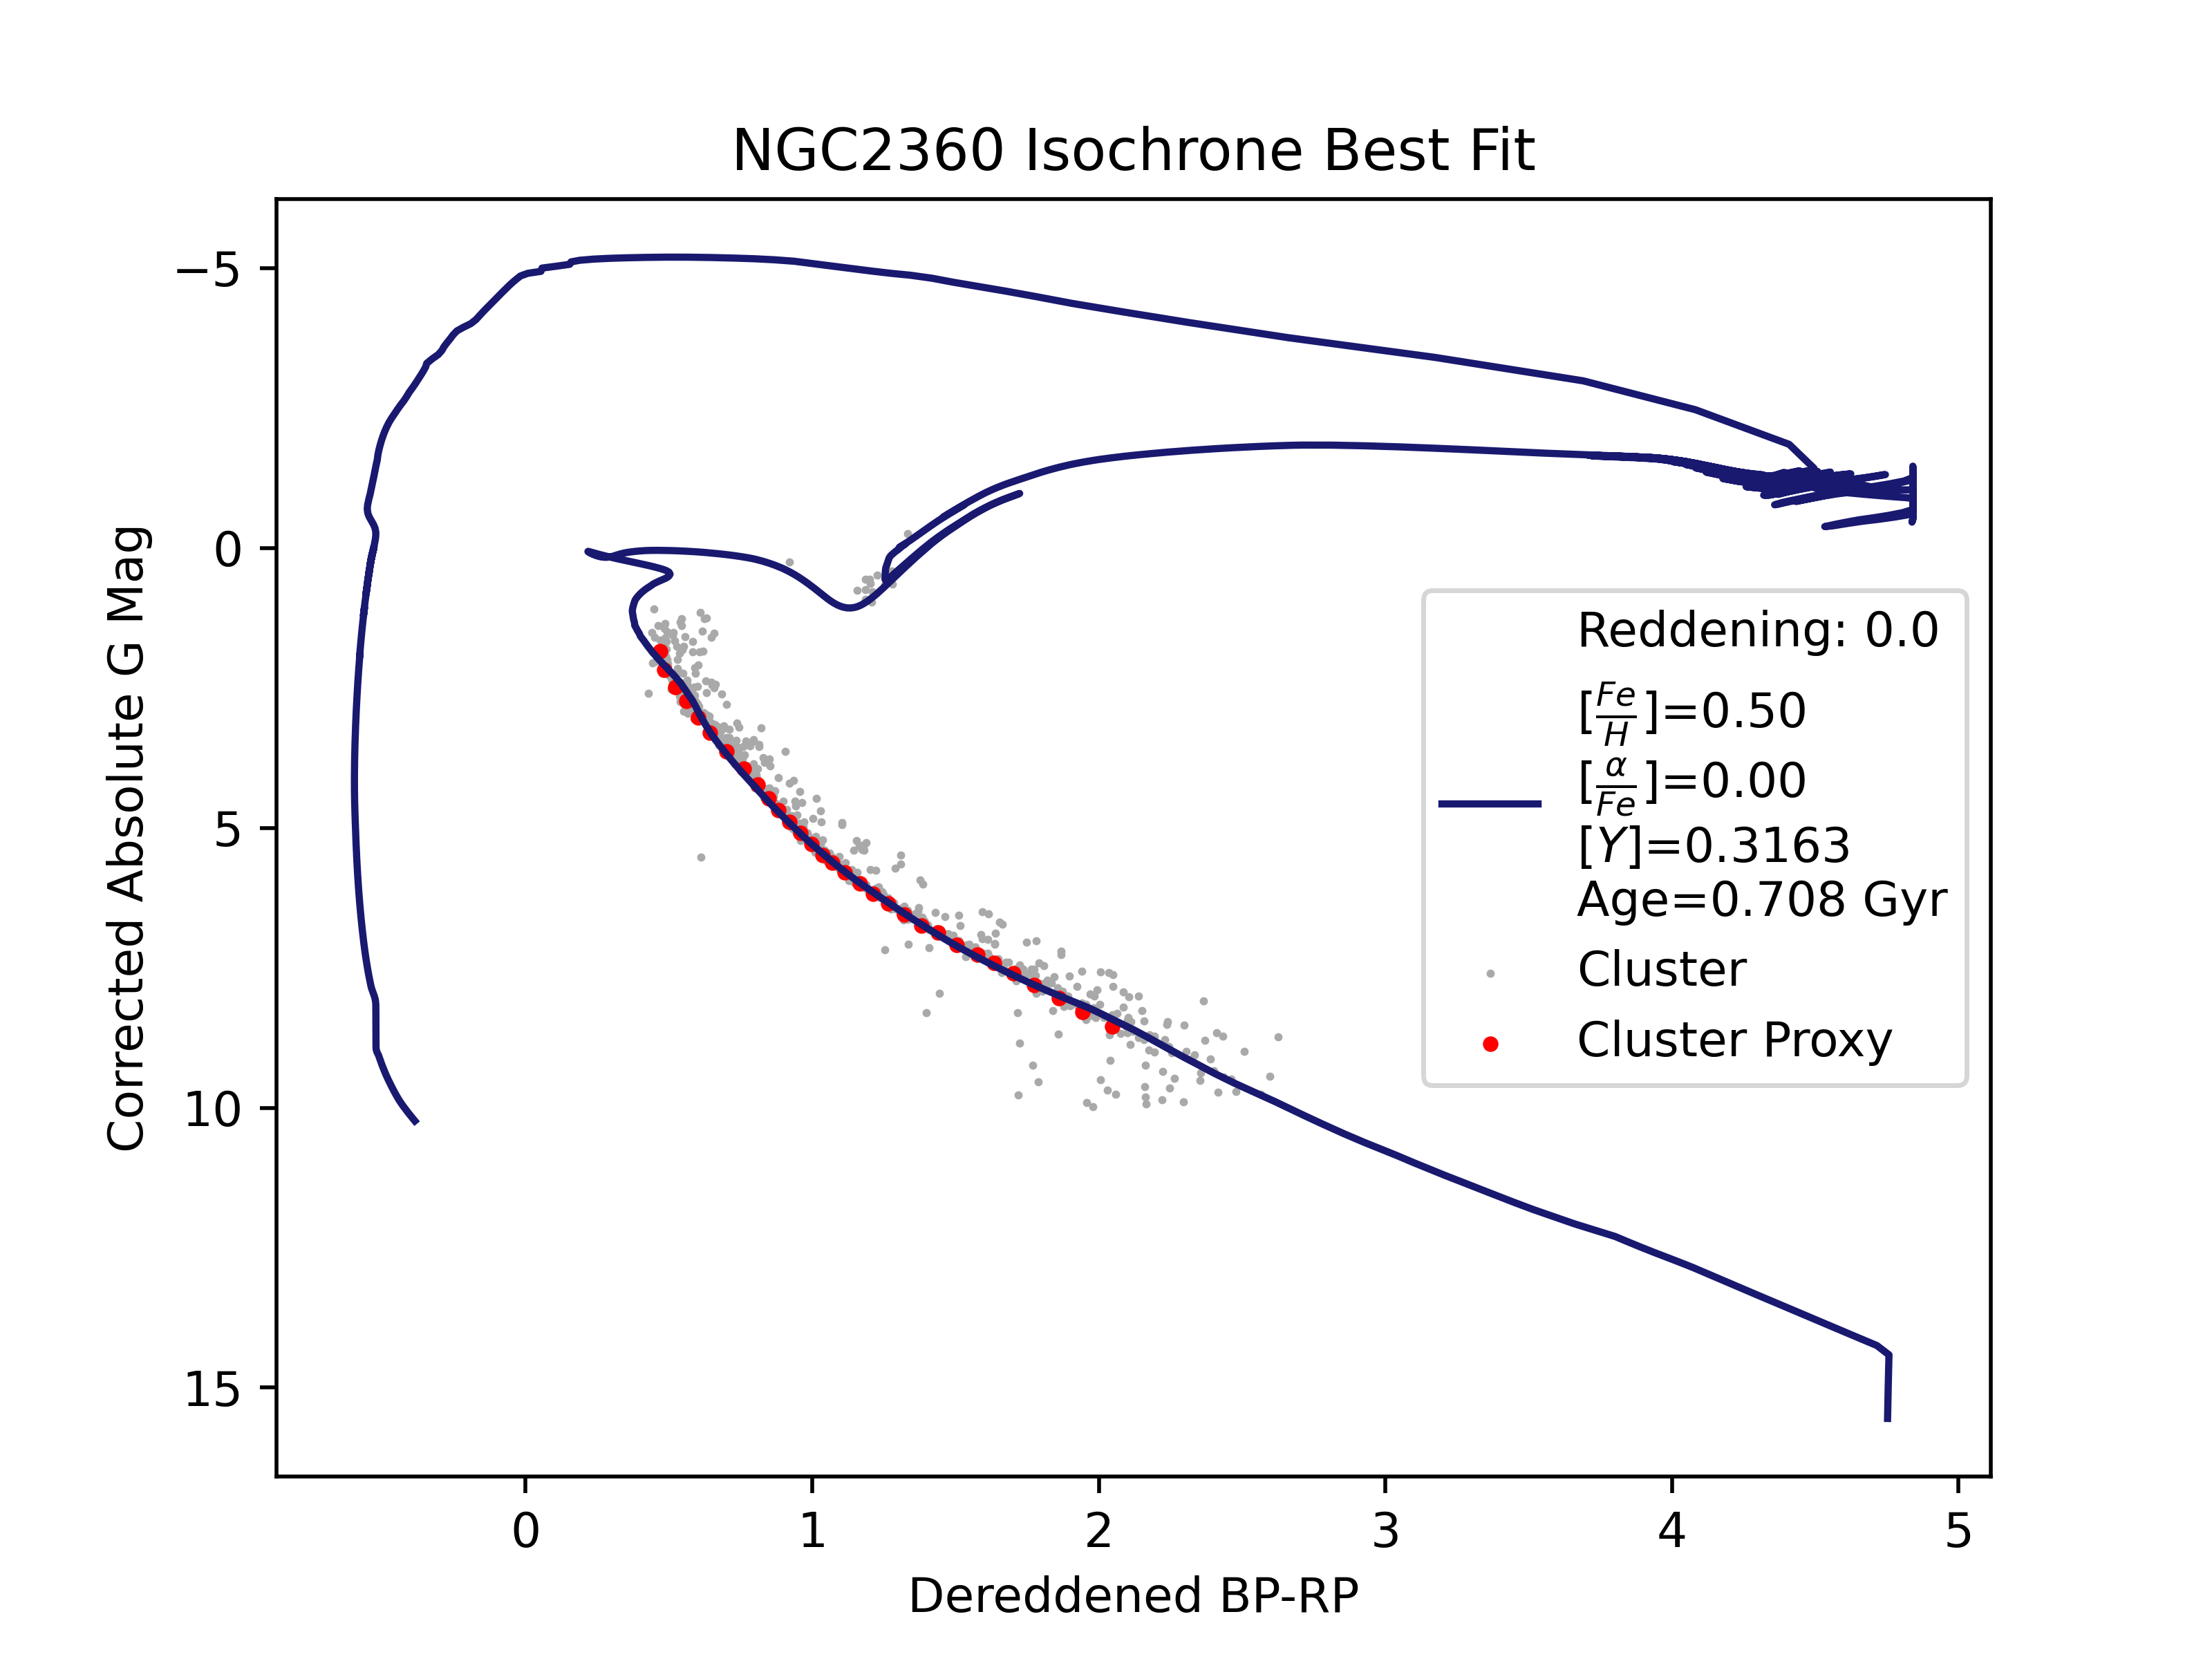
\includegraphics[width=4.75in]{figures/NGC2360_CMD_Iso_BestFit.png}
    \caption{Filtered, distance corrected, and interstellar reddening/extinction corrected CMD of NGC2360 shown in gray. The red points are proxy points used in the fitting process for efficiency. The best fitting isochrone is overlaid in dark blue.}
    \label{fig:NGC2360_iso}
\end{figure}


\section{Population Statistics} \label{sec:pop}

Our primary science goal, having grown in scope alongside that of the project and the number of clusters it surveys, is to analyze trends in the Milky Way's population of open clusters, and quantitatively characterize those trends. One such trend of interest is to empirically establish a relationship between the age of a cluster and the average mass of stars that it contains, through non-spectroscopic means. This utilizes both empirical observations and theoretical models, combining cluster membership identification with isochrone fitting for mass estimates. In theory, as a given cluster ages, higher mass stars will die off faster than lower mass stars. This means that we should expect to observe a correlation between the age of a cluster and the average mass of the stars it contains, all other variables equal. Unfortunately however, Figure \ref{fig:mass_vs_age_filtered} shows this trend to not be the case, or at least not easily observed. As for why, we have to consider the limits of Gaia's instrumentation.

\begin{figure}[]
    \centering
      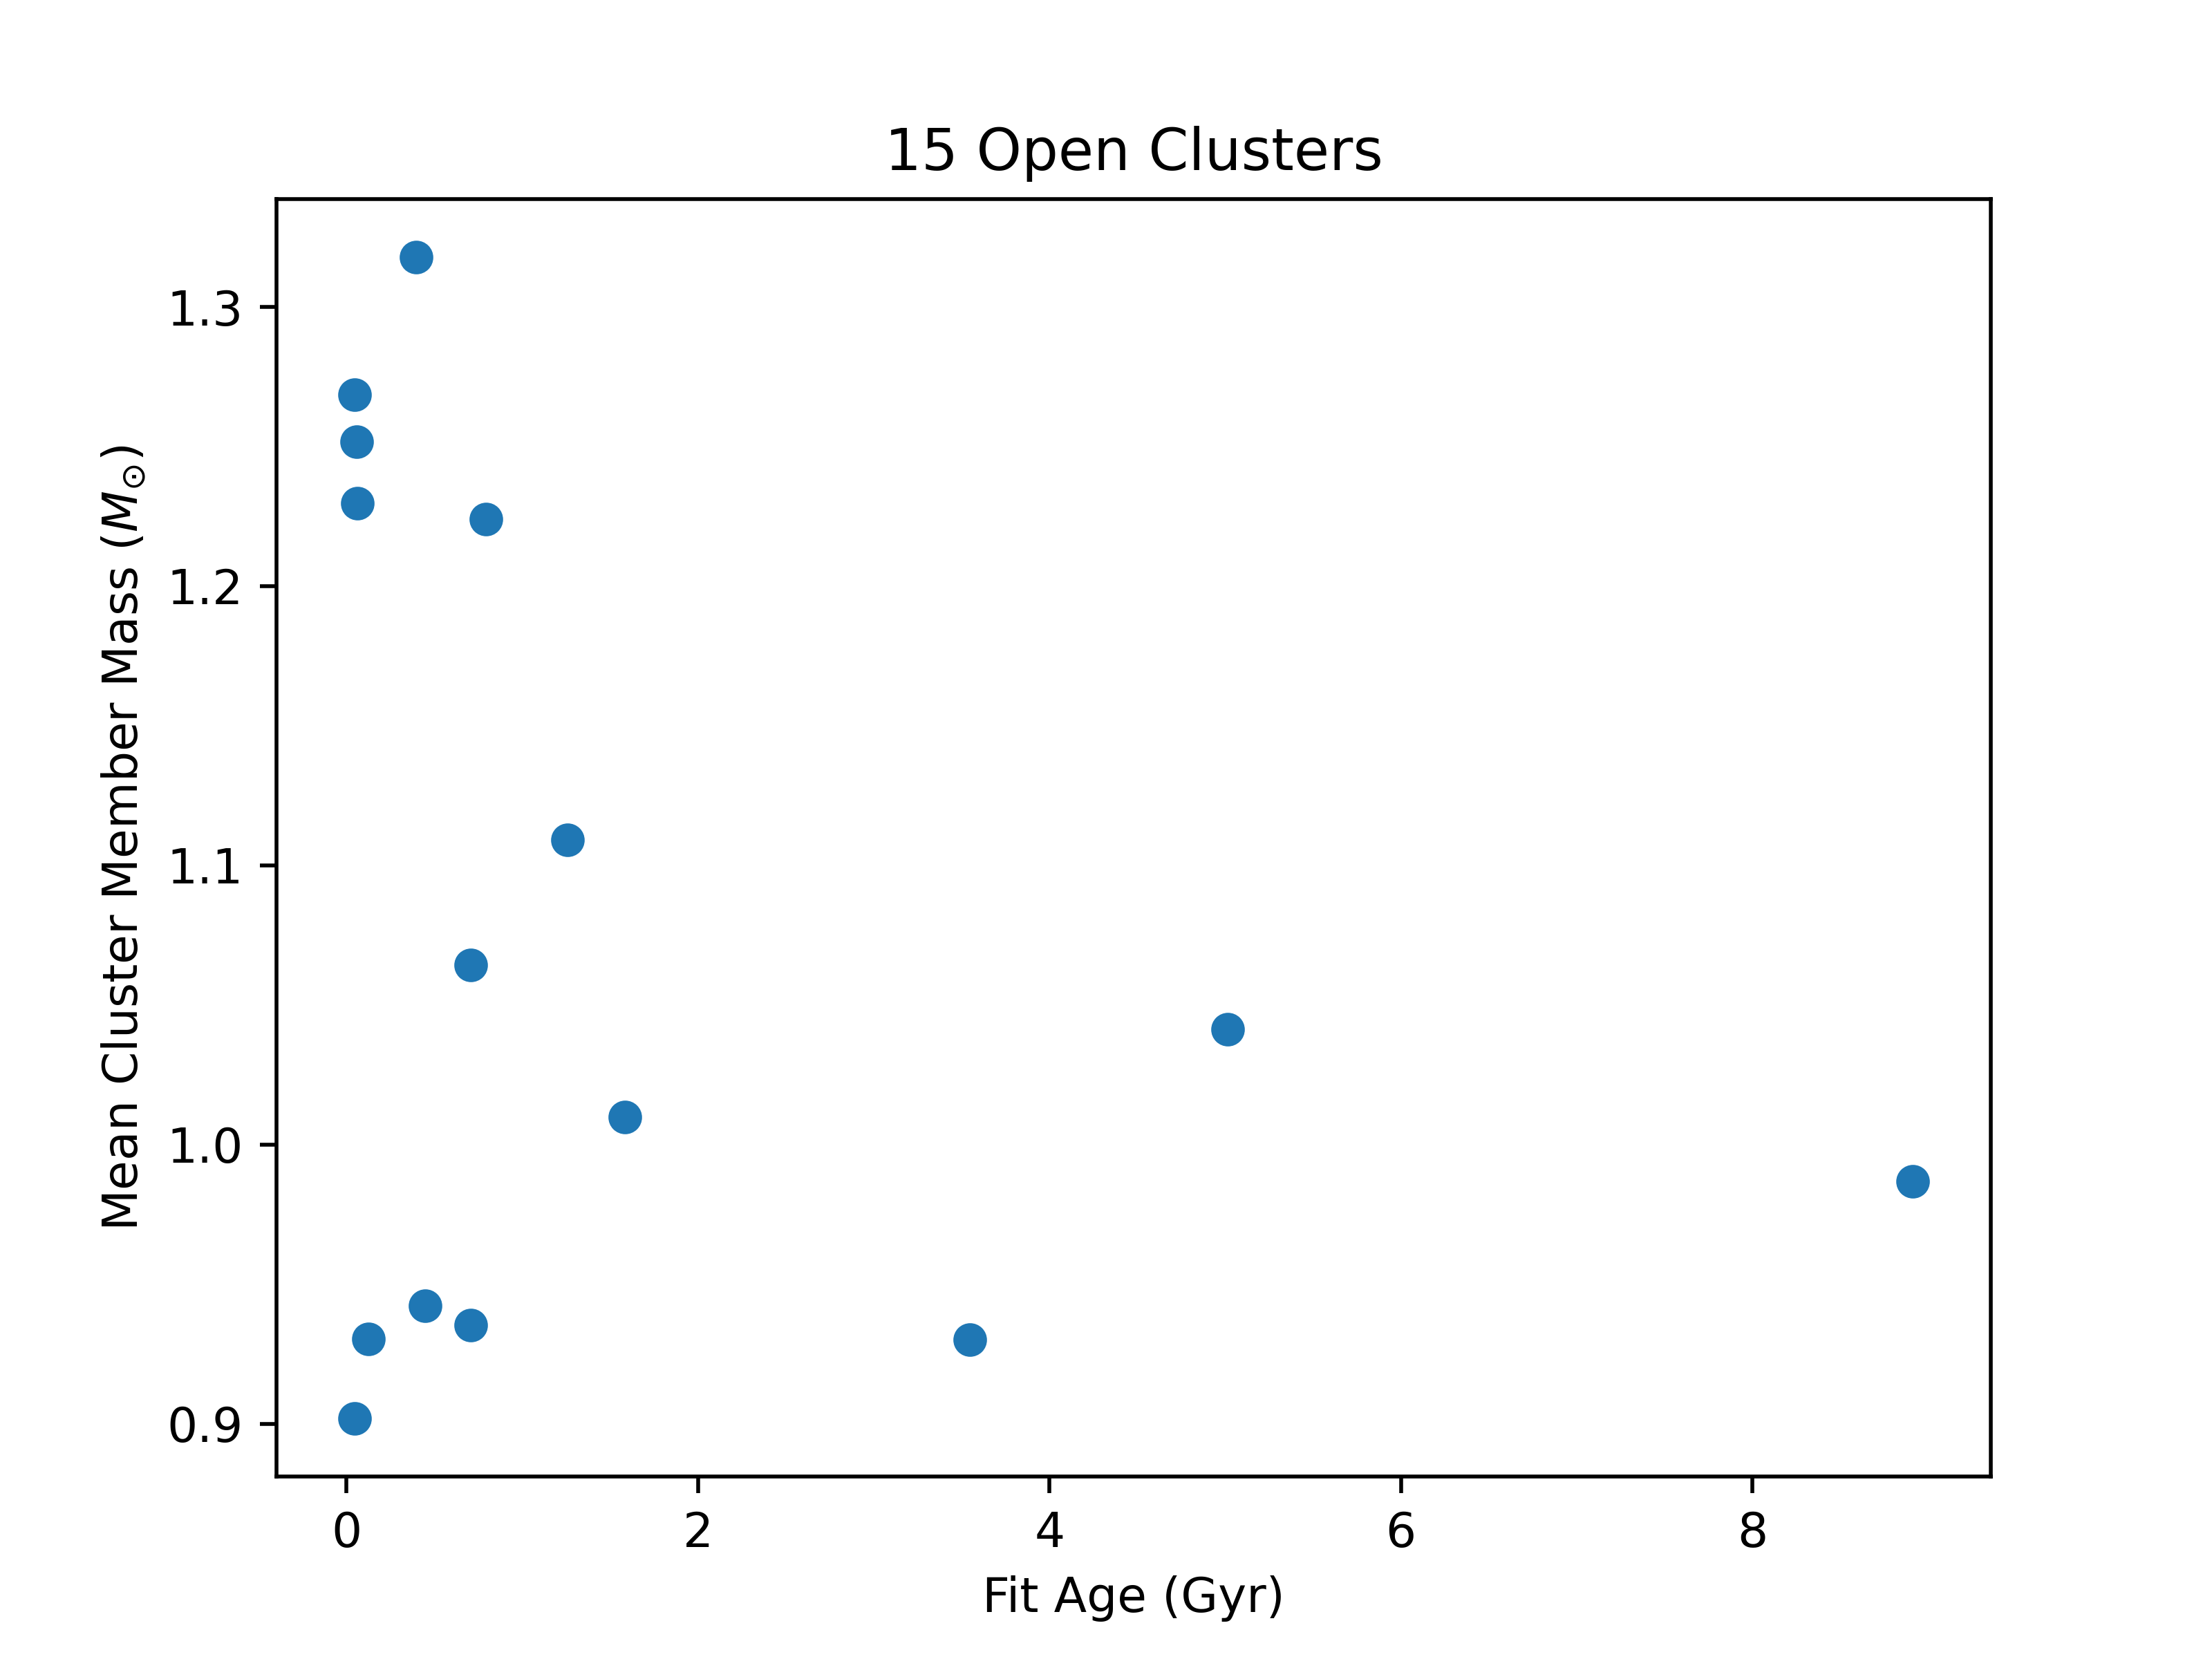
\includegraphics[width=4.75in]{figures/mass_vs_age_filtered.png}
    \caption{Average cluster member mass as a function of cluster age in 15 different open clusters. The full list of clusters included can be seen in the legend in Figure \ref{fig:pop_cmd_absolute}. No discernible correlation is apparent, with our working hypothesis being that this is due to the effects of a detector limit selection effect.}
    \label{fig:mass_vs_age_filtered}
\end{figure}

As discussed in Section \ref{sec:bias}, we believe that the brightness limits of Gaia's detectors may impart a selection bias in our cluster membership data by way of filtering out the fainter, lower main sequence. This selection bias would differentially affect individual clusters based on how dimly they are observed, both from interstellar extinction and from the effects of the inverse square law. In other words, clusters more distant from us will have their lower main sequence cut off prematurely when compared to more proximate clusters. It would follow, then, that any attempts to observe trends in cluster populations would need to account for this bias in the data.

Our solution to this bias has been to apply a filter on all data sets to the lower main sequence that is brighter than the cut that appears in the faintest cluster. To do this, we again refer to Figure \ref{fig:pop_cmd_absolute} and the limit we discussed in Section \ref{sec:bias}. Using the upper limit of de-reddened $BP-RP = 1.6$, we look again at the idea of an empirical age-mass relationship. In Figure \ref{fig:mass_vs_age_bounded}, this time a trend emerges. In general, we find that the average mass decreases as a function of the cluster's age. The absence of this trend in the full, uncut data set suggests that other mass related population statistics may be sensitive to the selection effect as well. We have so far been unsucessful in characterizing a model profile to fit accurately to the results of Figure \ref{fig:mass_vs_age_bounded}, but we highlight future plans to do so in Section \ref{sec:future}.

Reproducing the average stellar mass versus age relationship in a slightly different manner, Figure \ref{fig:mass_intercept_bounded_vs_age} compares the y-intercept of the average mass fit for each cluster as a function of age. This intercept value translates to the average stellar mass at the core of a cluster, and as such reflects similar characteristics to that of Figure \ref{fig:mass_vs_age_bounded}. These results have again been filtered to reduce selection bias, and the correlation is absent in the unfiltered data.

\begin{figure}[]
    \centering
      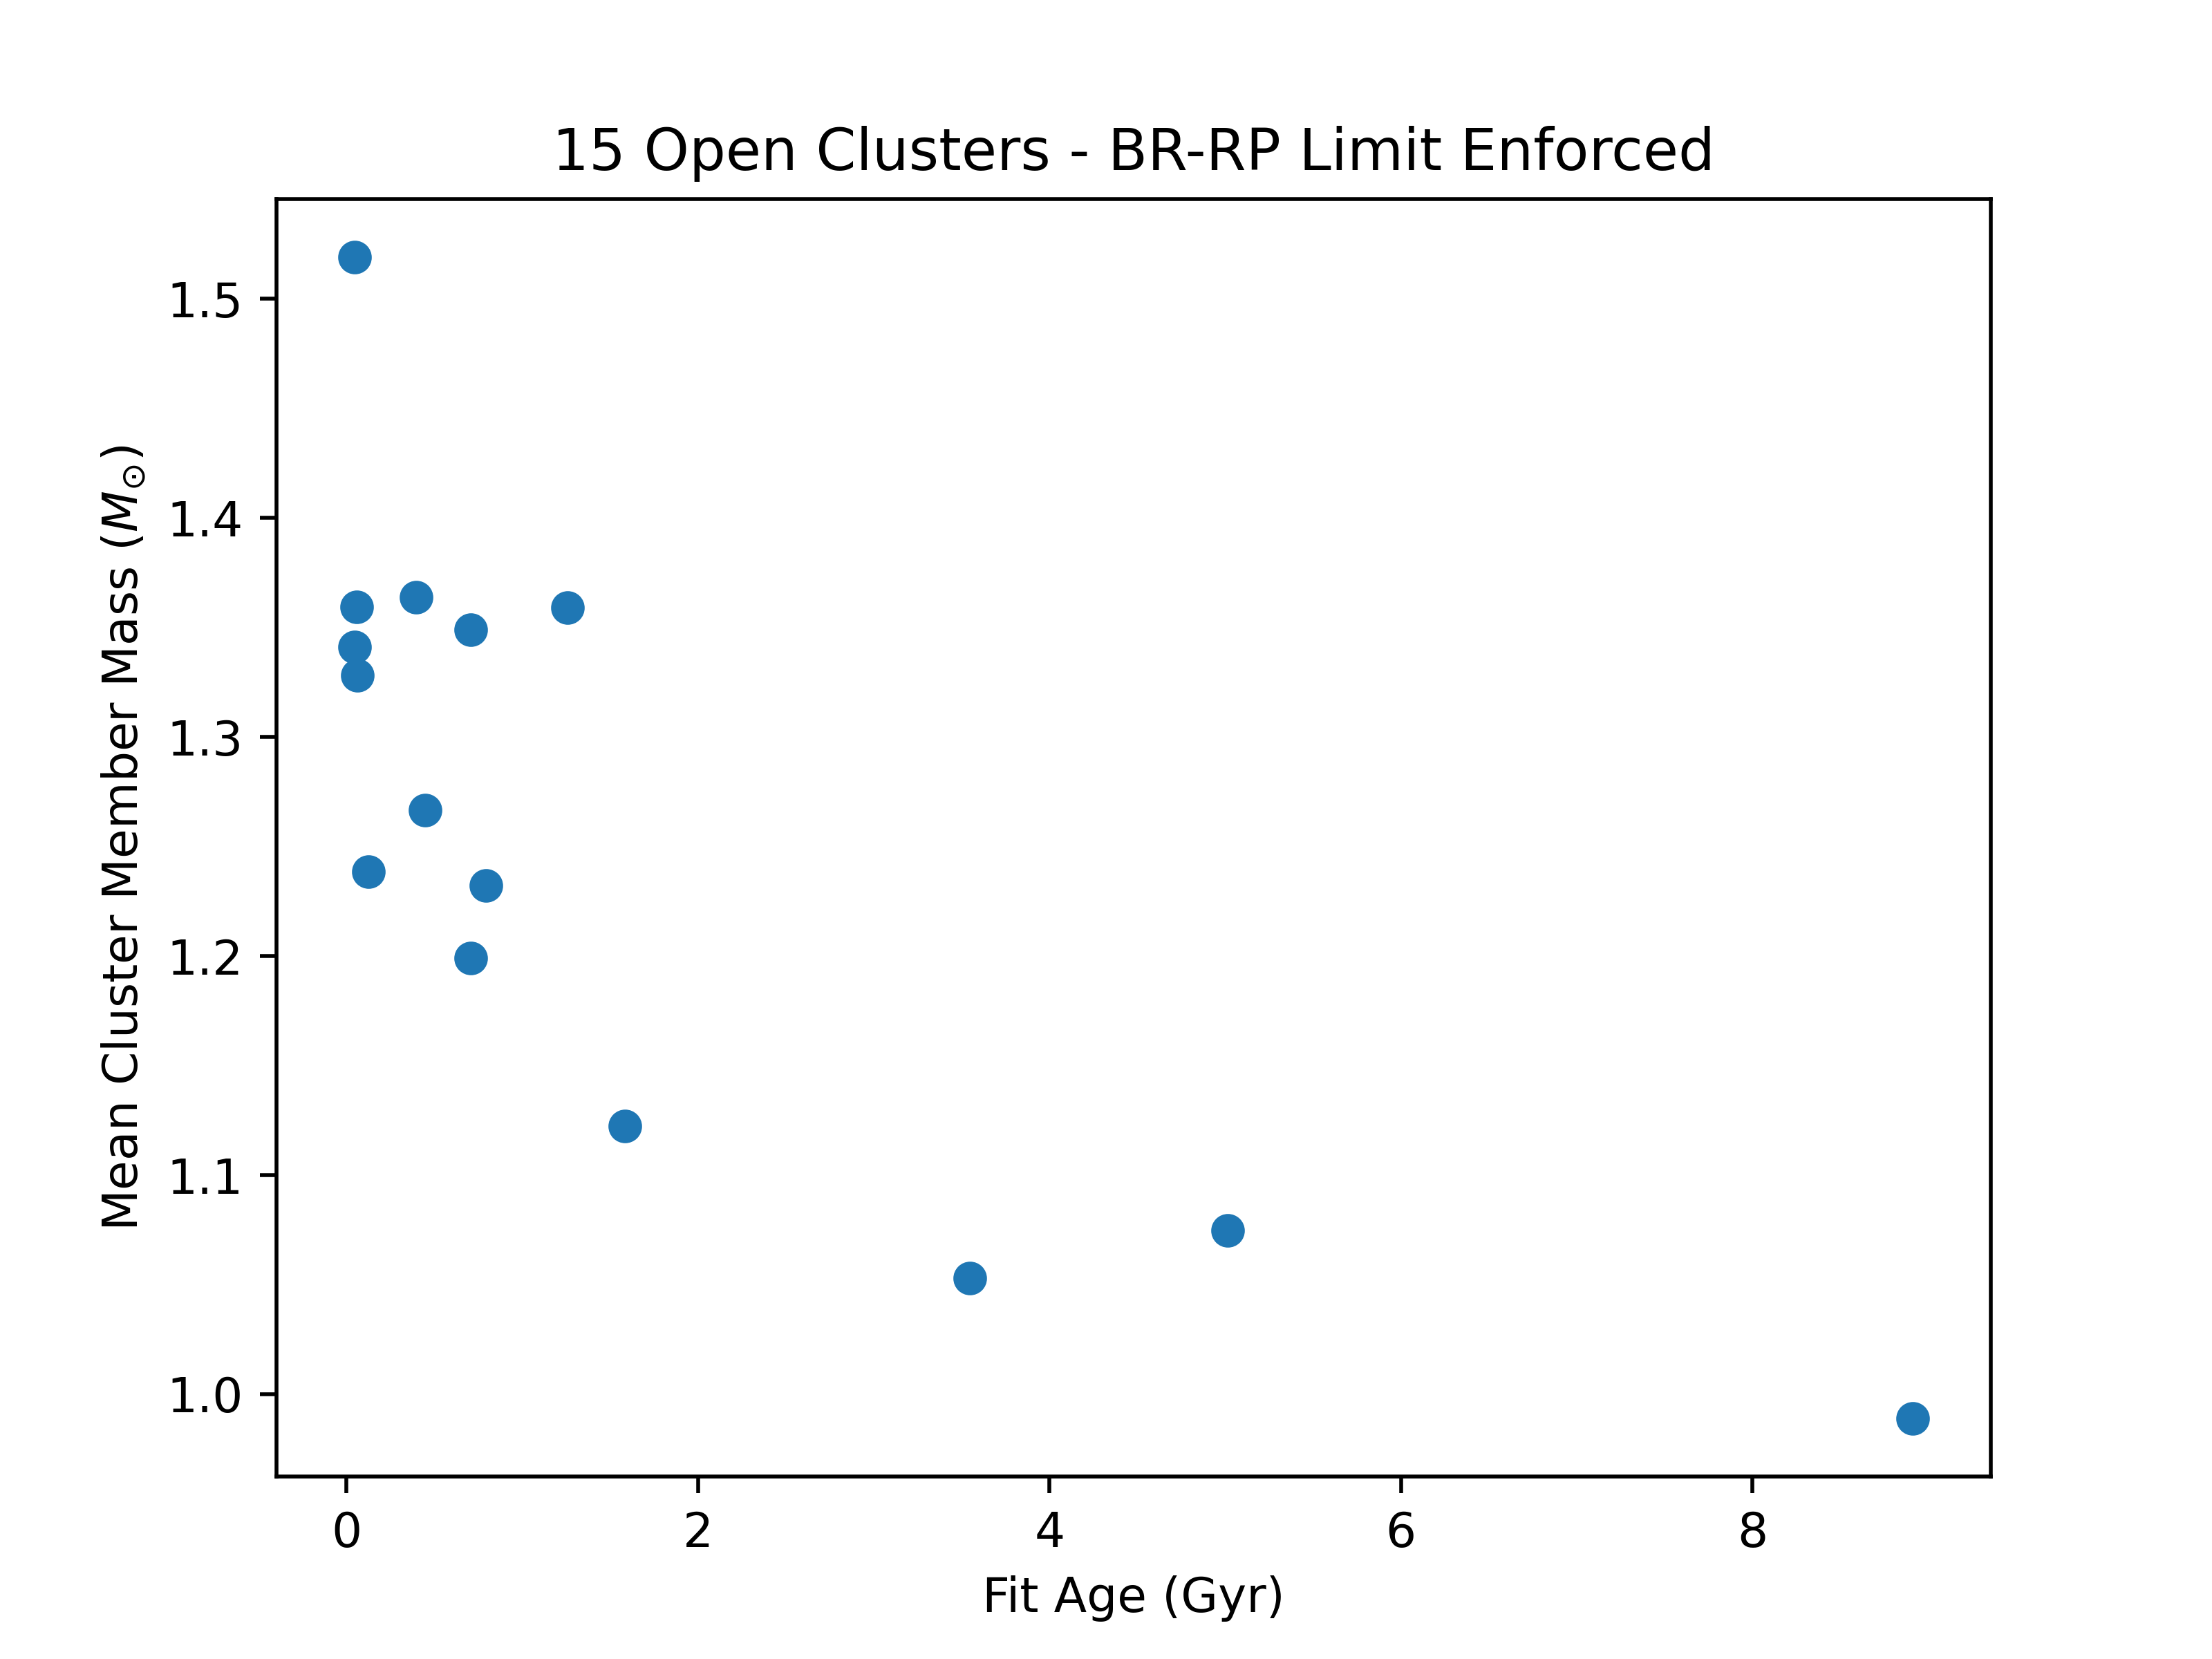
\includegraphics[width=4.75in]{figures/mass_vs_age_bounded.png}
    \caption{Average cluster member mass versus cluster age, for the same 15 clusters as in Figure \ref{fig:mass_vs_age_filtered}, but this time enforcing the $BP-RP = 1.6$ upper limit on each cluster. We assert that a correlation is visible, appearing somewhat exponential in nature. `Filling out' the region of the plot from 2Gyr to 8Gyr any more is quite difficult, as there are very few observed open clusters in the Milky Way which surpass 2Gyr in age.}
    \label{fig:mass_vs_age_bounded}
\end{figure}


To empirically visualize the effect that this selection bias has on the data, we can look at the differing effect that our manually enforced limit has on each cluster. Because observed brightness of a source diminishes as a function of the observing distance, we expect clusters further away to have a larger portion of their main sequence missing in observations due to the detector cutoff selection bias. This would mean that these further clusters would have less of their observed (i.e. post selection bias) main sequence affected by our limit of de-reddened $BP-RP = 1.6$. Figure \ref{fig:bounded_fraction_vs_dist} helps to visualize this trend, showing that the clusters least affected by the enforced color limit are indeed furthest from us. In other words, clusters at greater distances are already missing larger portions of their lower main sequence due to Gaia's detector limit.

As a way to anchor our data to known and well-studied phenomena, and to step away from population statistics focused on mass, we highlight the inverse square law in Figure \ref{fig:mag_vs_dist_bounded}. Note that the inverse square law, a relationship well documented, is for the relationship between light intensity and distance. In this case, the y-axis records magnitudes, which are a logarithmic scale of intensity. 

\begin{figure}[]
    \centering
      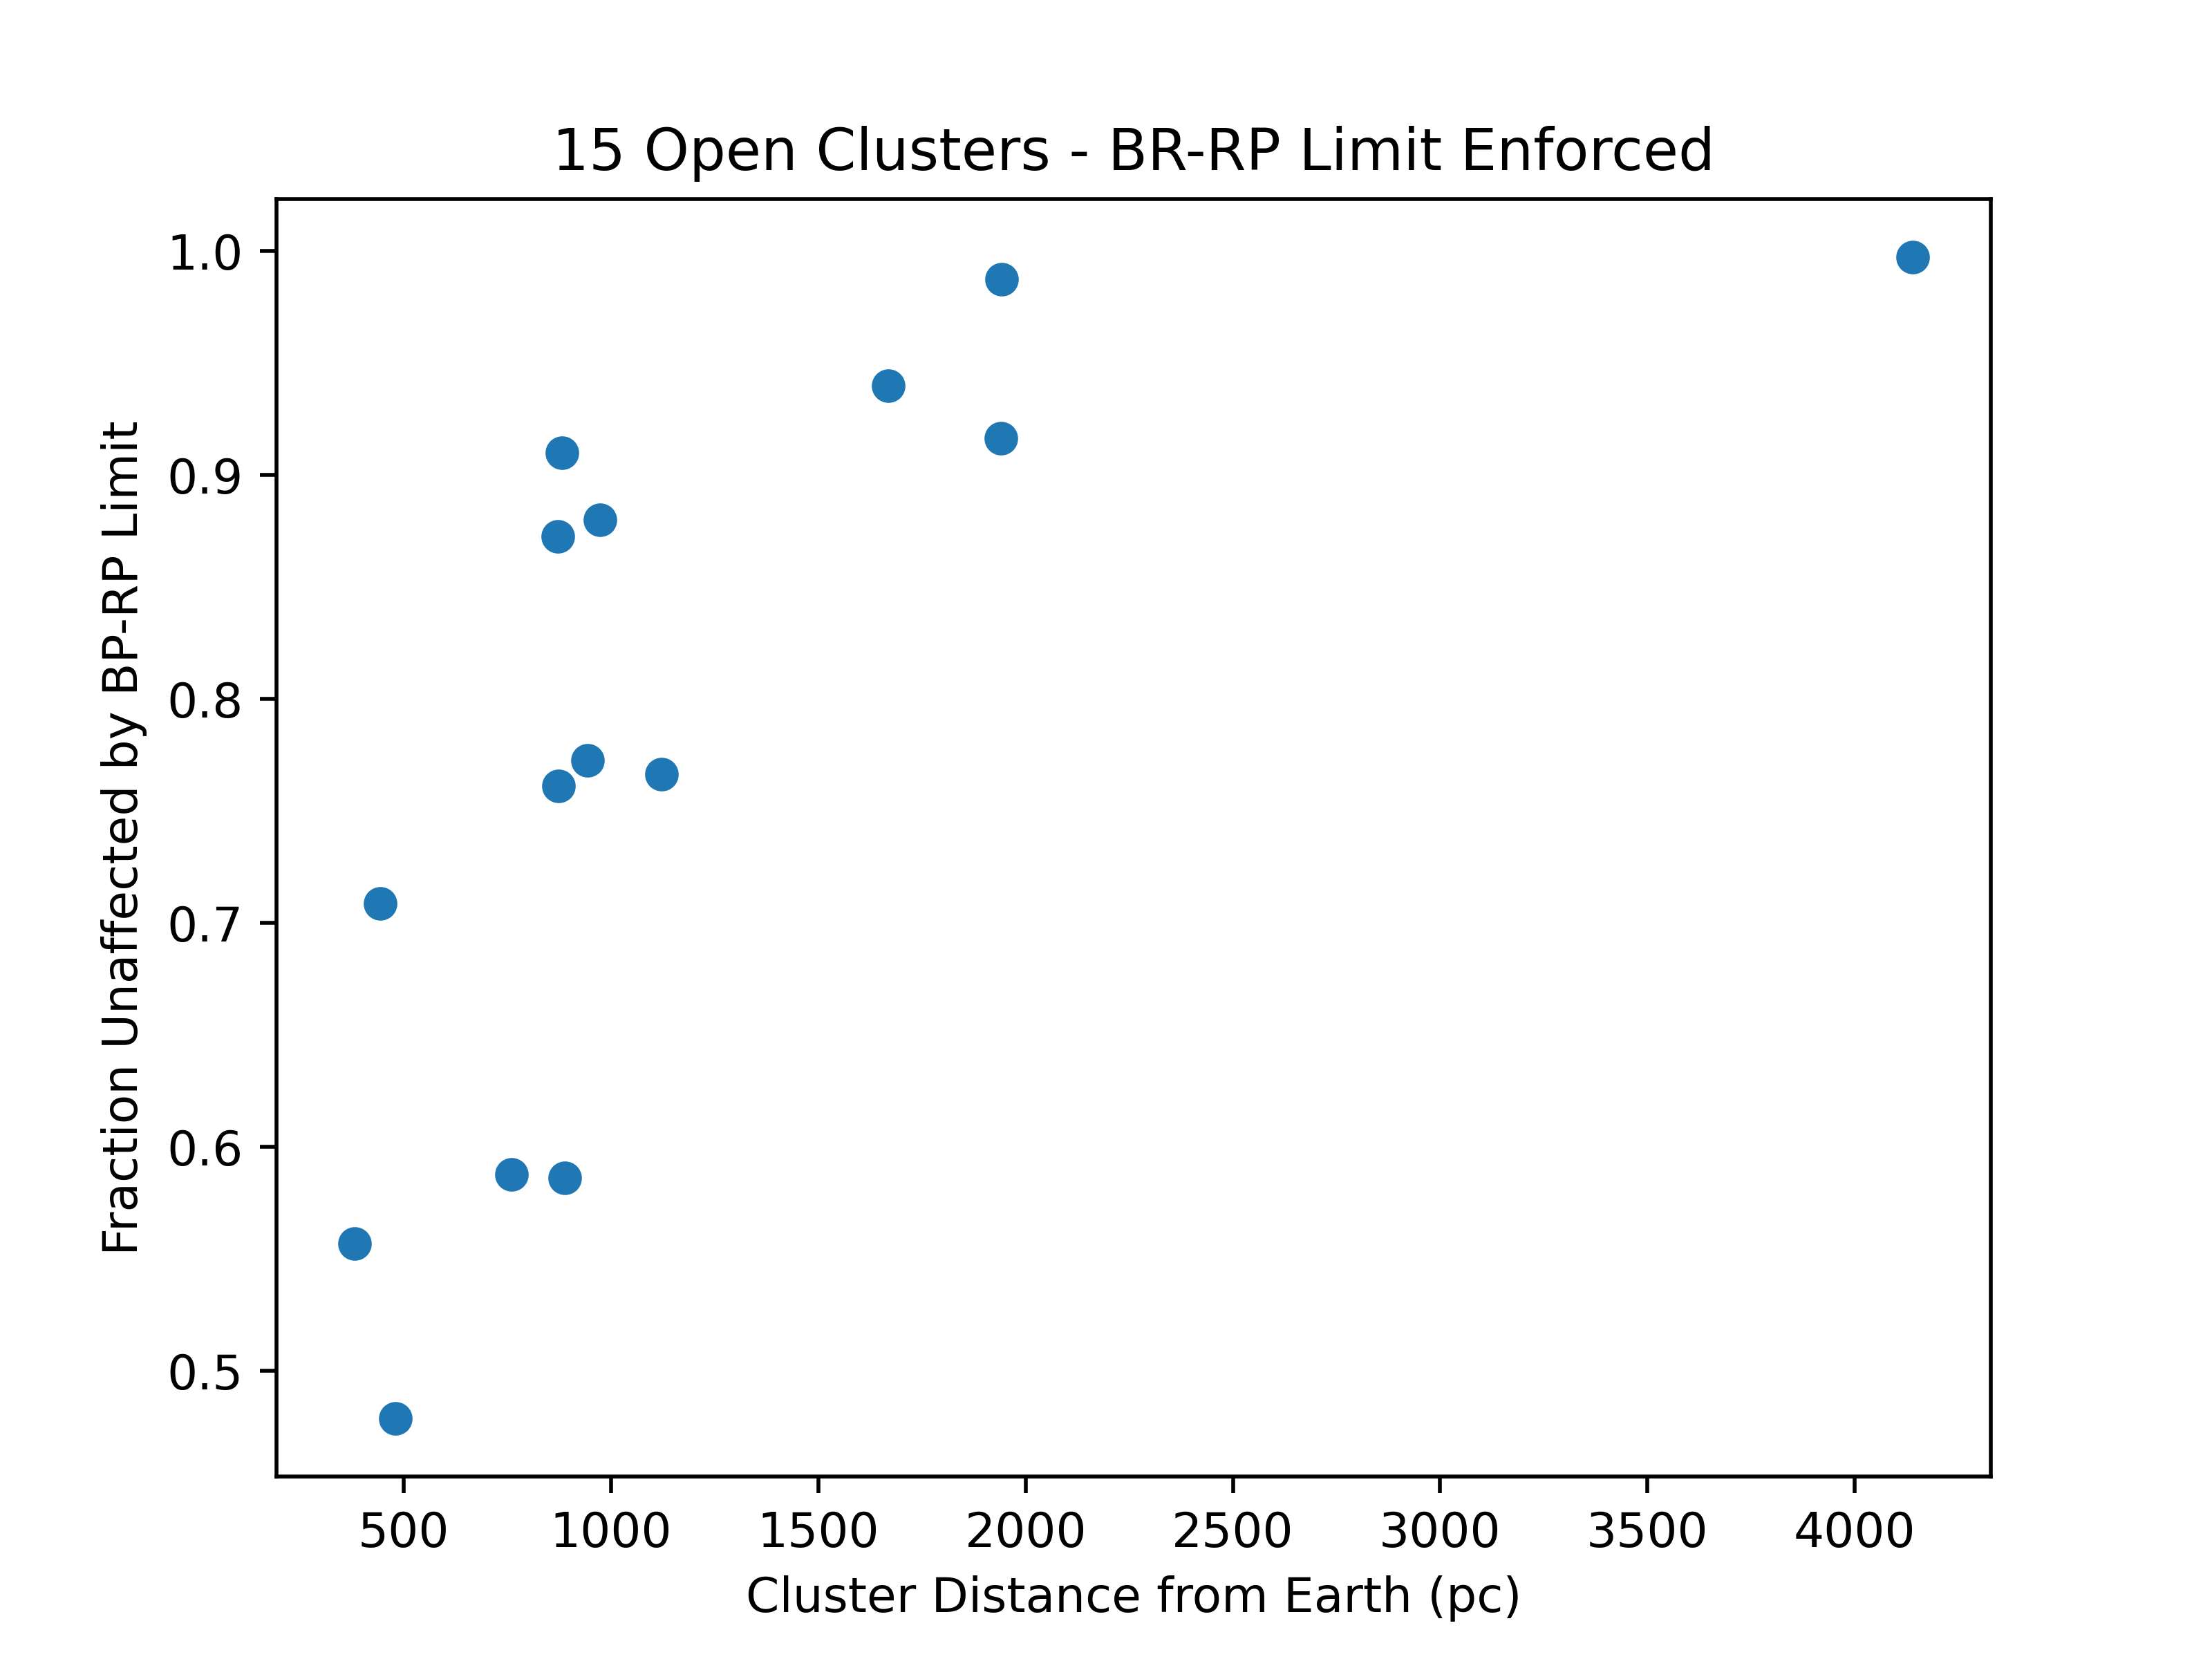
\includegraphics[width=4.75in]{figures/bounded_fraction_vs_dist.png}
    \caption{A visualization of the speculated selection effect from the detector limit of 21st magnitude. The y-axis tabulates the fraction of identified cluster members that are not thrown out by the upper limit of de-reddened $BP-RP = 1.6$ for each cluster. This means that the higher the y-value, the more of a cluster's lower main sequence is already missing in observations, likely due to the selection effect. Noise clipping in the cluster member filtering process is also expected to have minor effects on the fractions determined for a few of the clusters, though the overall trend persists.}
    \label{fig:bounded_fraction_vs_dist}
\end{figure}

\begin{figure}[]
    \centering
      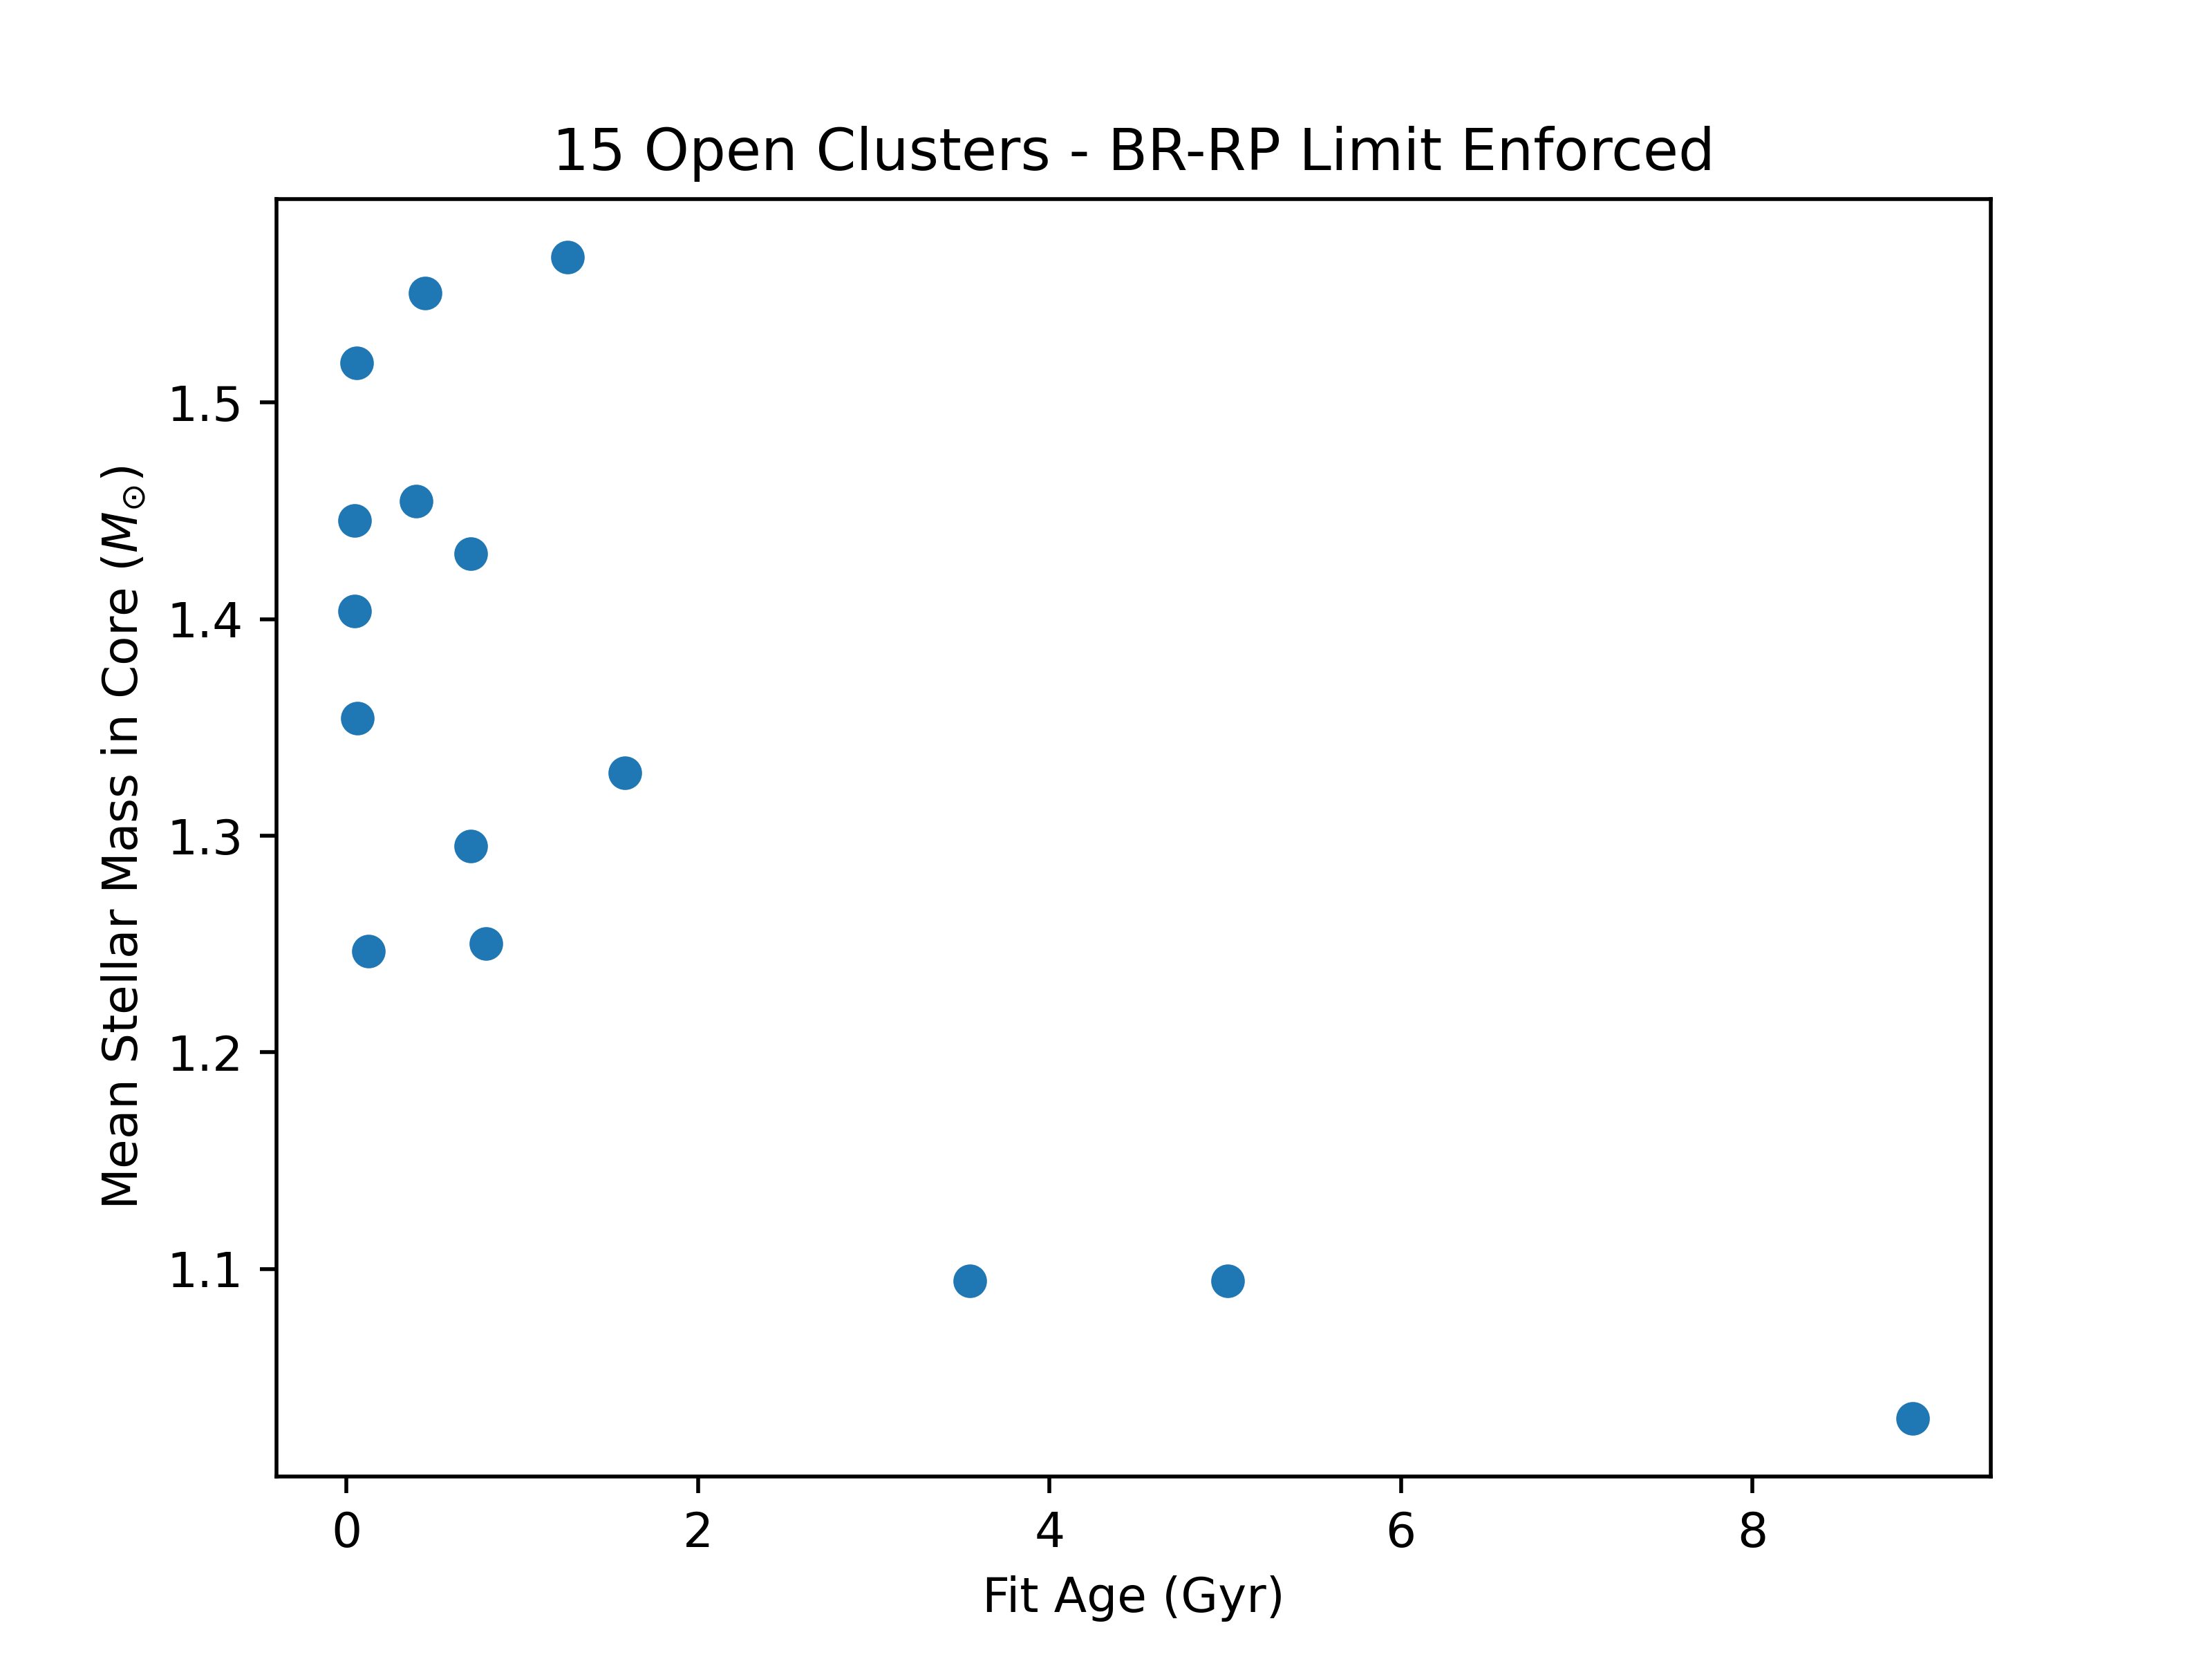
\includegraphics[width=4.75in]{figures/mass_intercept_vs_age_bounded.png}
    \caption{Y-axis tracks the intercept of the linear fit to the interquartile mean mass for each cluster, equivalent to the line determined in Figure \ref{fig:M67_average_mass_bounded}. Though the  $r^2$ value of the fit was low in the case of several clusters, the overall exponential-like correlation is still comparable to the one seen in Figure \ref{fig:mass_vs_age_bounded}.}
    \label{fig:mass_intercept_bounded_vs_age}
\end{figure}

\begin{figure}[]
    \centering
      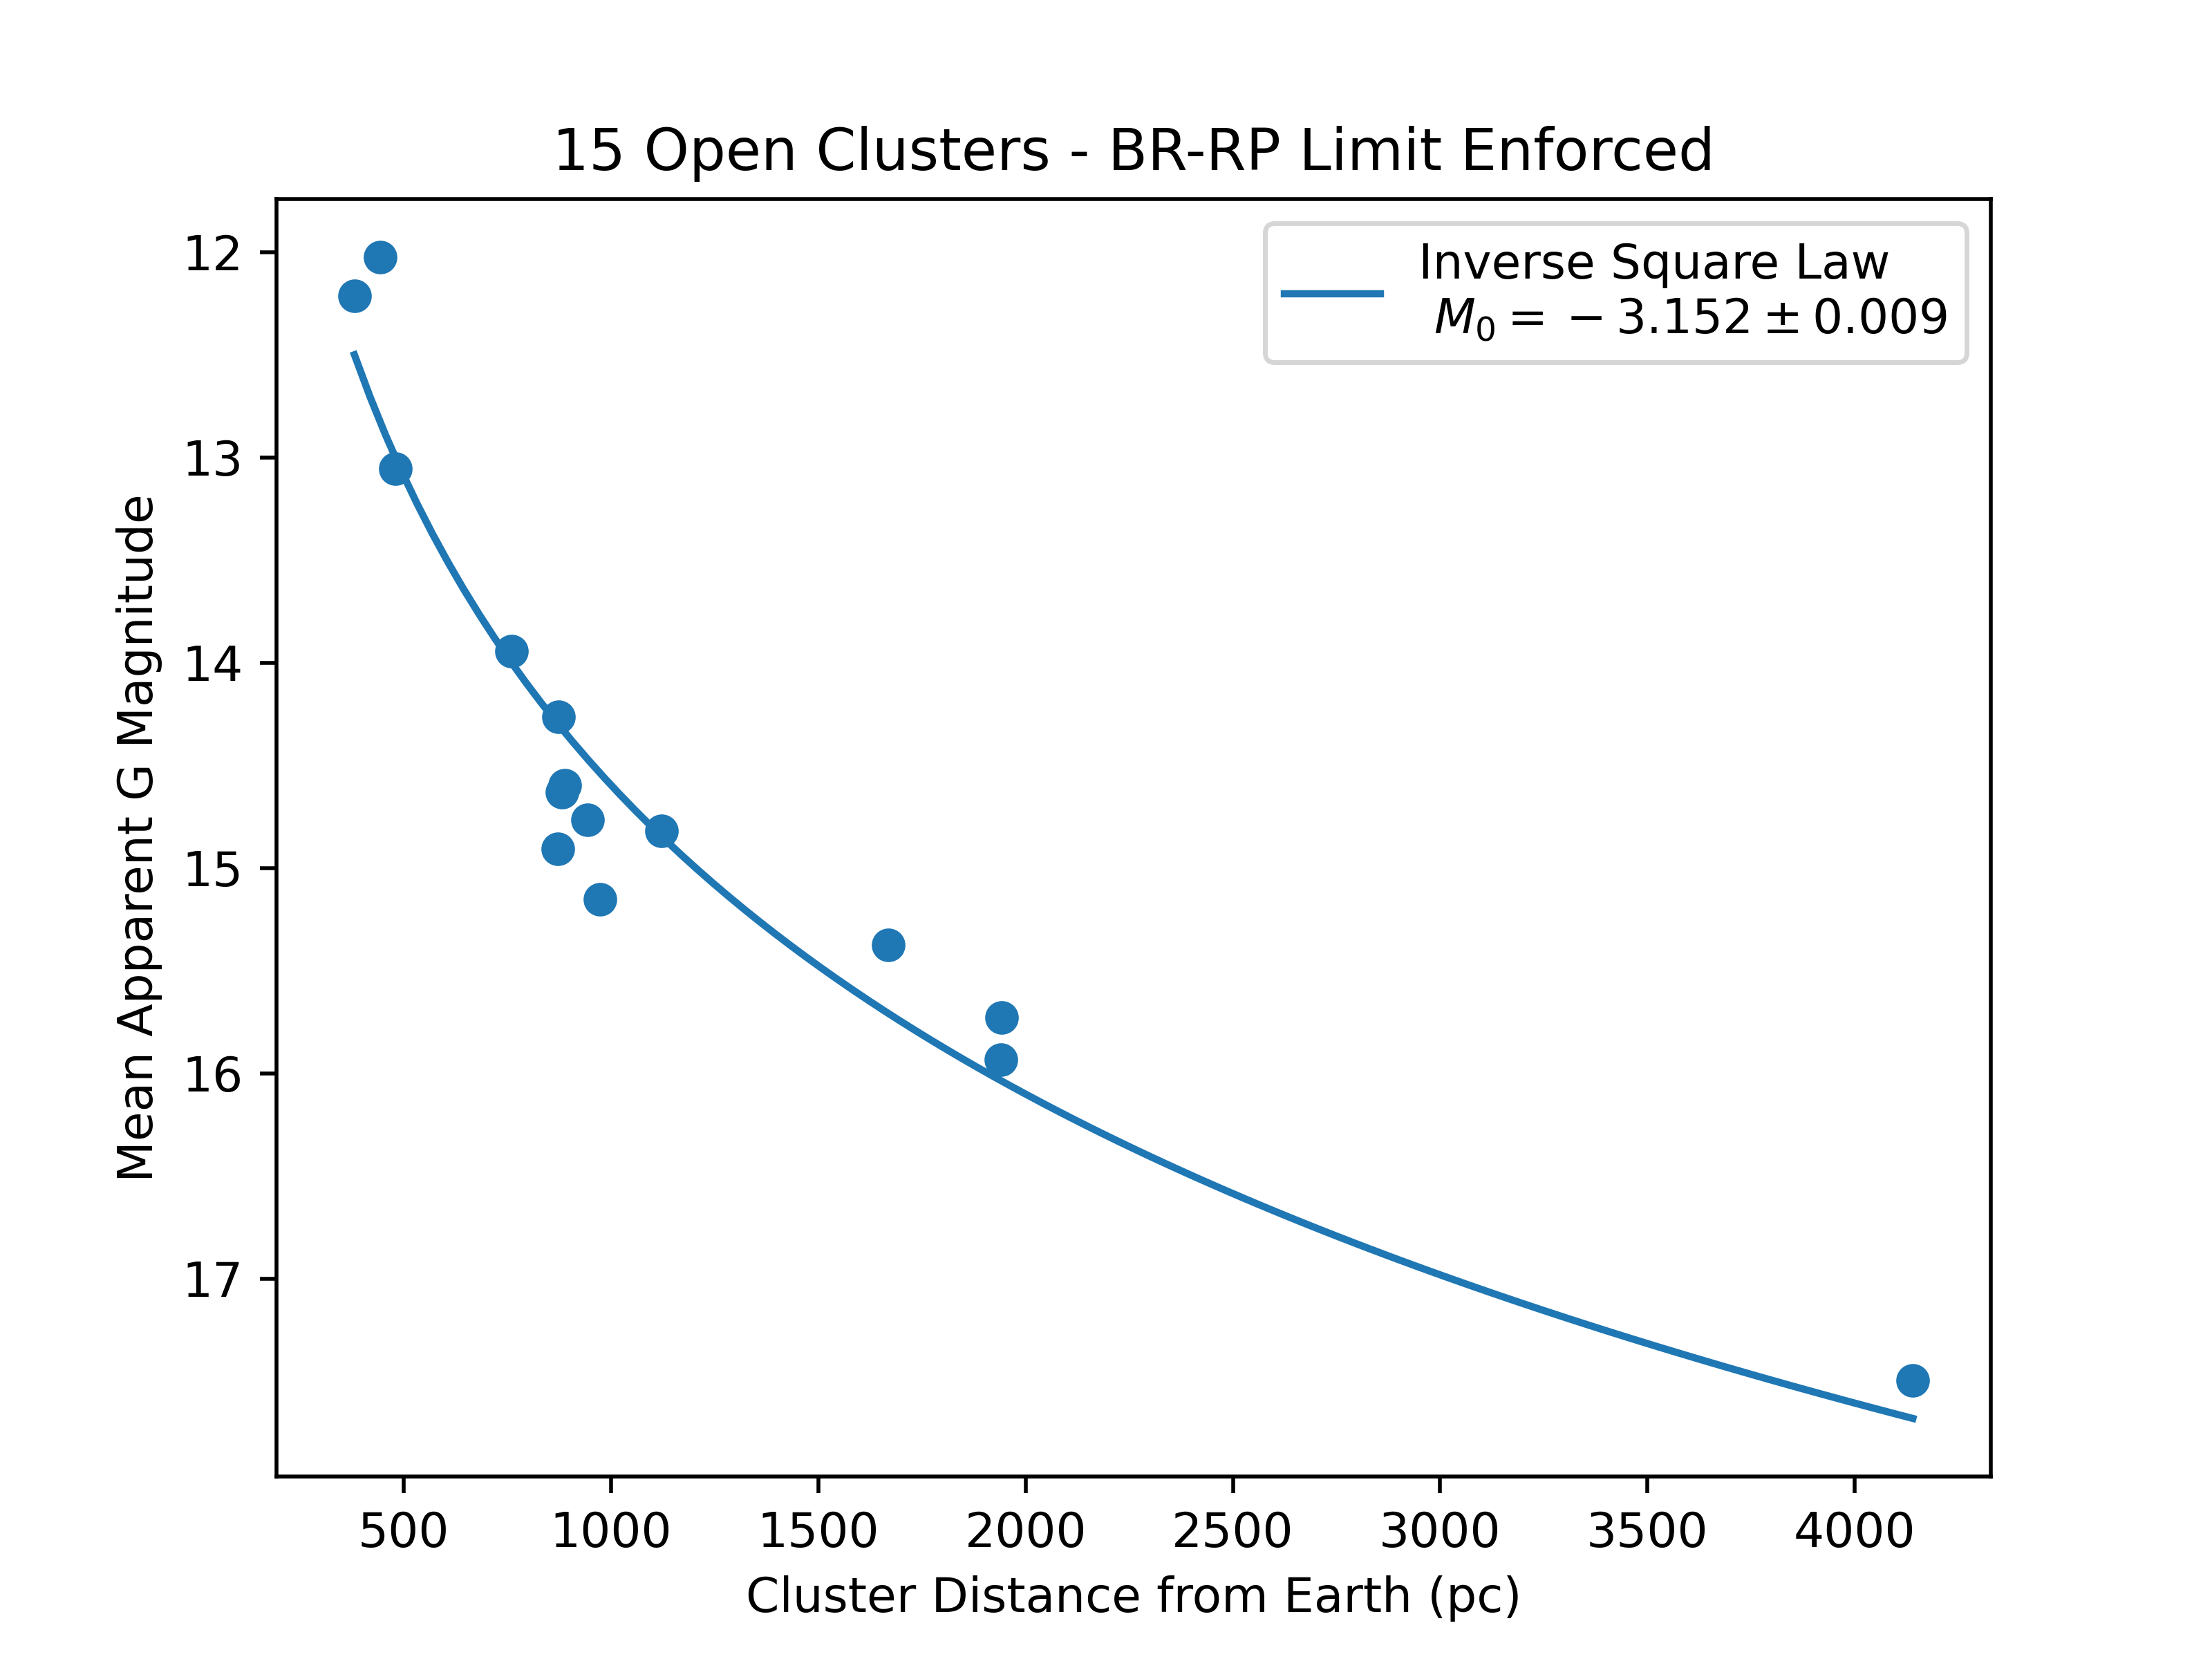
\includegraphics[width=4.75in]{figures/mag_vs_dist_bounded.png}
    \caption{A plot of the average G-band magnitude of limit-enforced stars in the 15 open clusters versus their distance from Earth. The expected relationship of the inverse square law is overlaid, and as expected is a good fit to the observed. This is not seen as a significant result of the paper, but rather an attempt to re-trace the known and assign some more validity to the methods used in this work.}
    \label{fig:mag_vs_dist_bounded}
\end{figure}

\section{Future Work} \label{sec:future}

Future work and improvements for this project fall into a few categories, the first of which being the isochrones used in the fitting process. We believe that MIST isochrones in their current iteration are some of the most robust and well-suited sets of synthetic isocrhones to our research. That said, they fall short in a few ares. Principally, the age determinations and alignments with globular clusters are reasonable but assumedly not accurate. For globular clusters with a literature age of 8-10 Gyr, the best fitting synthetic isochrones bear ages of order 15-20 Gyr. In addition, the current revision of MIST ischrones do not feature variance in $[\frac{\alpha}{Fe}]$, a component of metallicity that may improve the relative fit of an isochrone to observed data. In the cases of some open clusters, the lower main sequence diverges dramatically from the projected main sequence of the best-fitting isochrone, even when the rest of the main sequence and turnoff is fit perfectly. We hope that continued study of empirical open cluster CMDs with the precision of Gaia will lead to further refinements and revisions in synthetic isochrones.

Another primary avenue of improvement comes from a more robust filtering process, affecting the quality of end statistics, the efficiency of studying new clusters, and the ability to sample more clusters. Open clusters that lie in the plane of the galaxy, especially those with a lower stellar density, are prone to high fractions of line of sight contamination by non-cluster members. Gaia DR3 promises to bring radial velocity measurements to many more stars, potentially adding an extra dimension along which to identify cluster members. In addition, we think that the problem of identifying a boundary between cluster members and non-members as a function of multiple measurements is a task perfectly suited for several types of machine learning. As such, a combination of more information and a hands-on machine learning approach is something we'd consider to be a strong candidate for future improvement.

Another way of improving the filtering and cluster membership identification process is by adding more data. Radial velocity measurements would be likely to help increase our confidence in the final list of candidate cluster members. Given how important proper motion is in the filtering process, radial velocity measurements would quite literally add a whole new dimension. Gaia's full Data Release 3 is said to include radial velocity measurements for many more stars, though it is still possible that many potential cluster members will be lacking measurements. As such, if we are looking to further refine the filtering process, it makes sense to include other outside observations, including radial velocities and spectra, for some or all stars in a given cluster.

An area of future interest is closer analysis of the unresolved binary populations of open clusters. As mentioned in Section \ref{sec:dataUse}, many well filtered open clusters present a clear binary sequence. The best candidate cluster for this type of study would be Messier 67. In addition to have a low rate of non-member contamination and next to zero interstellar reddening, M67 demonstrates a clear binary sequence. While comparing the fractions of binary cluster members across different open clusters is not widely possible, owing to the lack of a clear binary sequence in some clusters, the well-filtered CMDs of clusters that do present clear binary sequences identify hundreds of unresolved binary candidates for further study using other surveys. Identifying the relative binary fraction in various open clusters would also allow for comparison to theory on binary formation and frequency as a function of other properties.

The extension of the methods and findings in this work to the Milky Way's population of globular clusters is something else we would like to include in future versions of this work. The primary reasons we are unable to delve into globular cluster population statistics currently are difficulties in the filtering and fitting procedures. Difficulties in the filtering process of globular clusters are ones that we hoped to see resolved by exploration of the aforementioned machine learning based filtering techniques. As for the ability to fit synthetic isochrones to the CMDs of globular clusters, it is something that we already posses the capability to do and have done for a handful of cases, but the ages given by best-fitting isochrones are nonphysical.

Finally, the most obvious and expected continuation of this work is to continue to process additional open clusters to increase the sample size and further refine the conclusions drawn in Section \ref{sec:pop}. Many of the trends and correlations observed and speculated in that section rely on a handful of points to draw a conclusion. While we assert that 15 open clusters is reaching the point of being statistically significant enough to start drawing conclusions, we would in no way turn down the opportunity to double or triple that number, even if it disproves any of our asserted findings. Gaia could resolve upwards of 5-7 times the number of open clusters included in this work, but the sampling of clusters over 2 Gyr is mostly limited to those sampled in this work. Altogether, we estimate that at least another 15-20 open clusters within 1 kpc of Earth could be analyzed in the same manner. We hope that at the very least, the methods and preliminary findings of this work help to pave future interest and work on the subject of delving into open stellar cluster population statistics.

\section{Acknowledgments}
I would like to thank Michael Richmond for his sage advice and guidance throughout the project, and his guidance as my advisor. I would also like to thank Joel Kastner for his insights and knowledge on young stellar clusters and main sequence tracks. Finally, I would like to thank RIT and the AST program in the School of Physics and Astronomy. Many of the faculty not individually named have been helpful to me in various stages of this research, and I would not have been able to complete this work without them.

This work has made use of data from the European Space Agency (ESA) mission
{\it Gaia} (\url{https://www.cosmos.esa.int/gaia}), processed by the {\it Gaia}
Data Processing and Analysis Consortium (DPAC,
\url{https://www.cosmos.esa.int/web/gaia/dpac/consortium}). Funding for the DPAC
has been provided by national institutions, in particular the institutions
participating in the {\it Gaia} Multilateral Agreement.

This research has made use of the SIMBAD database, operated at CDS, Strasbourg, France, \href{https://ui.adsabs.harvard.edu/abs/2000A\%26AS..143....9W}{2000,A\&AS,143,9} ,``The SIMBAD astronomical database", Wenger et al. 

\bibliography{Wainwright_Thesis}{}
\nocite{*}
\bibliographystyle{aasjournal}

\newpage{}
\appendix{}
In the interest of keeping down the page count, the hundreds of additional figures not included in this publication are available, along with the source code for the project, can be found on GitHub. In future, we also plan to include further documentation and guidance on use of the software, including a text-based tutorial and examples. 
\vspace{0.3cm}

Project Repository: \protect{\href{https://www.github.com/wjwainwright}{github.com/wjwainwright}}
\end{document}

